%%%%%%%%%%%%%%%%%%%%%%%%%%%%%%%%%%%%%%%%%%%%%%%%%%%%%%%%%%%%%%%%%%%%%
%
%   Este proyecto de Latex se ha creado a partir de la plantilla
%   de Jose Manuel Requena Plens (Universidad de Alicante) para la 
%   realización de mi TFM. En el siguiente enlace se puede encontrar
%   dicha plantilla:
%       
%       [+] github.com/jmrplens/TFG-TFM_EPS
%
%  	  - Autor:   David Carrascal <davidcawork@gmail.com>
%	  - Fecha:   20 Octubre 2022
%%%%%%%%%%%%%%%%%%%%%%%%%%%%%%%%%%%%%%%%%%%%%%%%%%%%%%%%%%%%%%%%%%%%%

%%%%%%%%%%%%%%%%%%%%   Notas  TFM   %%%%%%%%%%%%%%%%%%%%
%
%   - Cuando ponemos un capitulo con \chapter*{} no lo saca en el índice
%   
%


%%%%%%%%%%%%%%%%%%%%   Config  TFM   %%%%%%%%%%%%%%%%%%%%
\def\OptimizaTikZ{1} % On

% Config documento general, paquetes y demás

%%%%%%%%%%%%%%%%%%%%%%%%
% FORMATO DEL DOCUMENTO
%%%%%%%%%%%%%%%%%%%%%%%%
% scrbook es la clase de documento
% Si se desea que no haya página en blanco entre capítulos añadir "openany" en los parámetros de la clase. Sino siempre los capítulos empezarán en página impar.
\documentclass[a4paper,11pt,titlepage]{scrbook}
\KOMAoption{toc}{bib,chapterentryfill} % Opciones del índice
\usepackage{scrhack} % Previene algunos errores
% Paquete de formato para scrbook. Con marcas, linea-separador superior e inferior
\usepackage[automark,headsepline,footsepline]{scrlayer-scrpage}
\clearpairofpagestyles		% Borra los estilos por defecto
%%
% Formato y contenido de la información de cabecera y pie de página
%%
% Información de capítulo en cabecera e interno
\ihead{{\color{gray30}\scshape\small\headmark}}
% Número de página en cabecera y externo
\ohead{\normalfont\pagemark}
% Número de página en pie de página y externo. Sólo en páginas sin cabecera
\ofoot[\normalfont\pagemark]{}
%% 		
% Edición del contenido de las distintas partes de la cabecera
%%
\renewcommand{\chaptermark}[1]{\markboth{#1}{}} % Capítulo (Solo texto)
\renewcommand{\sectionmark}[1]{\markright{\thesection. #1}} % Sección (Número y texto)
\setkomafont{pagenumber}{} % Número de página (Sin nada añadido)

% Añade al índice y numera hasta la profundidad 4.
% 1:section,2:subsection,3:subsubsection,4:paragraph
\setcounter{tocdepth}{4}
\setcounter{secnumdepth}{4}
% Muestra una regla para comprobar el formato de las páginas
%\usepackage[type=upperleft,showframe,marklength=8mm]{fgruler}
% MÁRGENES DE LAS PÁGINAS
\usepackage[
  inner	=	3.0cm, % Margen interior
  outer	=	2.7cm, % Margen exterior
  top	=	2.5cm, % Margen superior
  bottom=	2.5cm, % Margen inferior
  includeheadfoot, % Incluye cabecera y pie de página en los márgenes
]{geometry}
% Valor de interlineado
\renewcommand{\baselinestretch}{1.2} % 1 línea de interlineado
% Para poder generar páginas horizontales
\usepackage{lscape}
% Ancho de la zona para comentarios en el margen. (modificado para todonotes)
\setlength{\marginparwidth}{1.9cm}

%%%%%%%%%%%%%%%%%%%%%%%%
% BIBLIOGRAFÍA
%%%%%%%%%%%%%%%%%%%%%%%%
%\usepackage{apacite} % NORMA APA
\usepackage[numbers]{natbib}
\usepackage{breakcites,notoccite}

%%%%%%%%%%%%%%%%%%%%%%%%
% DOCUMENTO EN ESPAÑOL
%%%%%%%%%%%%%%%%%%%%%%%%
\usepackage[base]{babel}
\usepackage{polyglossia}
\setdefaultlanguage{spanish}

\addto\captionsspanish{%
  \renewcommand{\listtablename}{Índice de tablas}
  \renewcommand{\tablename}{Tabla}
  \renewcommand{\lstlistingname}{Código}
  \renewcommand{\lstlistlistingname}{Índice de \lstlistingname s}
  \renewcommand{\glossaryname}{Glosario}
  \renewcommand{\acronymname}{Acrónimos}
  \renewcommand{\bibname}{Bibliografía}%
}

%%%%%%%%%%%%%%%%%%%%%%%% 
% COLORES
%%%%%%%%%%%%%%%%%%%%%%%% 
% Biblioteca de colores
\usepackage{color}
\usepackage[table,xcdraw,dvipsnames]{xcolor}
% Otros colores definidos por el usuario
\definecolor{gray97}{gray}{.97}
\definecolor{gray75}{gray}{.75}
\definecolor{gray45}{gray}{.45}
\definecolor{gray30}{gray}{.30}
\definecolor{negro}{RGB}{0,0,0}
\definecolor{blanco}{RGB}{255,255,255}
\definecolor{dkgreen}{rgb}{0,.6,0}
\definecolor{dkblue}{rgb}{0,0,.6}
\definecolor{dkyellow}{cmyk}{0,0,.8,.3}
\definecolor{gray}{rgb}{0.5,0.5,0.5}
\definecolor{mauve}{rgb}{0.58,0,0.82}
\definecolor{deepblue}{rgb}{0,0,0.5}
\definecolor{deepred}{rgb}{0.6,0,0}
\definecolor{deepgreen}{rgb}{0,0.5,0}
\definecolor{MyDarkGreen}{rgb}{0.0,0.4,0.0}
\definecolor{bluekeywords}{rgb}{0.13,0.13,1}
\definecolor{greencomments}{rgb}{0,0.5,0}
\definecolor{redstrings}{rgb}{0.9,0,0}

%%%%%%%%%%%%%%%%%%%%%%%%
% TABLAS
%%%%%%%%%%%%%%%%%%%%%%%%
% Paquetes para tablas
\usepackage{longtable,booktabs,array,multirow,multicol,tabularx,ragged2e,array}
\usepackage{graphicx}

% Nuevos tipos de columna para tabla, se pueden utilizar como por ejemplo C{3cm} en la definición de columnas de la función tabular
\newcolumntype{L}[1]{>{\raggedright\let\newline\\\arraybackslash\hspace{0pt}}m{#1}}
\newcolumntype{C}[1]{>{\centering\let\newline\\\arraybackslash\hspace{0pt}}m{#1}}
\newcolumntype{R}[1]{>{\raggedleft\let\newline\\\arraybackslash\hspace{0pt}}m{#1}}

%%%%%%%%%%%%%%%%%%%%%%%% 
% GRAFICAS y DIAGRAMAS 
%%%%%%%%%%%%%%%%%%%%%%%% 
% Paquete para todo tipo de gráficas, diagramas, modificación de imágenes, etc
\usepackage{rotating}
\usepackage{tikz,tikzpagenodes}
\usetikzlibrary{tikzmark,calc,shapes.geometric,arrows,backgrounds,shadings,shapes.arrows,shapes.symbols,shadows,positioning,fit,automata,patterns,intersections}
\usepackage{pgfplots}
\pgfplotsset{colormap/jet}
\pgfplotsset{compat=newest} % Compatibilidad
\usepgfplotslibrary{patchplots,groupplots,fillbetween,polar}
\usepackage{pgfplotstable}
% Guardar las figuras realizadas con Tikz y Pgf en una carpeta externa
% para agilizar el procesado y tenerlas para utilizarlas en otros
% documentos
\if\OptimizaTikZ 1
  \usepgfplotslibrary{external}
  \tikzset{%
    external/system call ={xelatex -enable-write18 -halt-on-error -interaction=batchmode -jobname "\image" "\texsource"},
  }
\fi

% Estilos para elementos graficos
% Cajas y cajas de texto
\tikzstyle{Caja1} = [green,very thick,rounded corners,fill=white, fill opacity=0.5]
\tikzstyle{Texto1} = [fill=white,thick,shape=circle,draw=black,inner sep=2pt,font=\sffamily,text=black]
\tikzstyle{Texto2} = [fill=white,thick,shape=rectangle,draw=black,inner sep=2pt,font=\sffamily,text=black]
\tikzstyle{Texto3} = [fill=white,thick,shape=circle,draw=black,inner sep=2pt,font=\sffamily,text=black]
% Cuadros de diagrama
\tikzstyle{rectvioleta} = [rectangle, rounded corners, text centered, draw=black, fill=blue!10]
\tikzstyle{rectnaranja} = [rectangle, minimum width=2cm, minimum height=1cm, text centered, draw=black, fill=orange!10]
\tikzstyle{romborosa} = [diamond, aspect=3, minimum width=3cm, minimum height=1cm, text centered, draw=black, fill=red!10]
\tikzstyle{rectverde} = [rectangle, minimum width=2cm, minimum height=1cm, text centered, draw=black, fill=green!10]
\tikzstyle{rectamarillo} = [rectangle, rounded corners, minimum width=2cm, minimum height=1cm, text centered, draw=black, fill=yellow!10]
% Flechas
\tikzstyle{arrow} = [thick,->,>=stealth]

%%%%%%%%%%%%%%%%%%%%%%%% 
% FIGURAS, TABLAS, ETC 
%%%%%%%%%%%%%%%%%%%%%%%% 
\usepackage{subcaption} % Para poder realizar subfiguras
\usepackage{caption} % Para aumentar las opciones de diseño
% Nombres de figuras, tablas, etc, en negrita la numeración, todo con letra small
\captionsetup{labelfont={bf,small},textfont=small}
% Paquete para modificar los espacios arriba y abajo de una figura o tabla
\usepackage{setspace}
% Define el espacio tanto arriba como abajo de las figuras, tablas
\setlength{\intextsep}{5mm}
% Para ajustar tamaños de texto de toda una tabla o grafica
% Uso: {\scalefont{0.8} \begin{...} \end{...} }
\usepackage{scalefnt}
% Redefine las tablas y figuras para eliminar el '.' entre la numeración y el texto
\renewcommand*{\figureformat}{\figurename~\thefigure}
\renewcommand*{\tableformat}{\tablename~\thetable}

% Para el diagrama de gantt del presupesto 
\usepackage{pgfgantt}

% Para las checkmarks and crossmarks in latex
\usepackage{amssymb}% http://ctan.org/pkg/amssymb
\usepackage{pifont}% http://ctan.org/pkg/pifont
\newcommand{\cmark}{\ding{51}}%
\newcommand{\xmark}{\ding{55}}%

%%%%%%%%%%%%%%%%%%%%%%%% 
% TEXTO
%%%%%%%%%%%%%%%%%%%%%%%%
% Paquete para poder modificar las fuente de texto
\usepackage{xltxtra}
% Cualquier tamaño de texto. Uso: {\fontsize{100pt}{120pt}\selectfont tutexto}
\usepackage{anyfontsize}
% Para modificar parametros del texto.
\usepackage{setspace}
% Paquete para posicionar bloques de texto
\usepackage{textpos}
% Paquete para realizar cajas de texto. 
% Uso: \begin{mdframed}[linecolor=red!100!black] tutexto \end{mdframed}
\usepackage{framed,mdframed}
% Para subrayar. Uso: \hlc[tucolor]{tutexto}
\newcommand{\hlc}[2][yellow]{ {\sethlcolor{#1} \hl{#2}} }

%% queremos emojis!!!
\usepackage{fontspec}
\newfontfamily\DejaSans{DejaVu Sans}

%%%%%%%%%%%%%%%%%%%%%%%% 
% OTROS
%%%%%%%%%%%%%%%%%%%%%%%%
% Para hacer una pagina horizontal. Uso: \begin{landscape} xxxx \end{lanscape}
\usepackage{lscape}
% Para incluir paginas PDF. Uso:
% \includepdf[pages={1}]{tuarchivo.pdf}
\usepackage{pdfpages}
% Para introducir url's con formato. Uso: \url{http://www.google.es}
\usepackage{url}
% Amplia muchas funciones graficas de latex
\usepackage{graphicx}
% Paquete que añade el hipervinculo en referencias dentro del documento, indice, etc
% Se define sin bordes alrededor. Uso: \ref{tulabel}
\usepackage[pdfborder={000}]{hyperref}
\usepackage{float}
\usepackage{placeins}
\usepackage{afterpage}
\usepackage{verbatim}
% Paquete para condicionales avanzados
\usepackage{xstring,xifthen}
% Paquete para realizar calculos en el código
\usepackage{calc}
% Para rotar tablas o figuras o su contenido
\usepackage{rotating}
% Para incluir comentarios en el texto. El parámetro 'disable' oculta todas las notas.
% USO: \todo{tutexto}
\usepackage[textsize=tiny,spanish,shadow,textwidth=2cm]{todonotes}
%\reversemarginpar % Descomentar si se quiere todos los comentarios en el mismo lado
% Desactiva la exportación de los ToDo y Missingfigures como figuras
\if\OptimizaTikZ 1
  \makeatletter
  \renewcommand{\todo}[2][]{\tikzexternaldisable\@todo[#1]{#2}\tikzexternalenable}
  \makeatother
  \usepackage{letltxmacro}
  \LetLtxMacro{\oldmissingfigure}{\missingfigure}
  \makeatletter
  \renewcommand{\missingfigure}[2][]{\tikzexternaldisable\oldmissingfigure[{#1}]{#2}\tikzexternalenable}
  \makeatother
\fi

%%%%%%%%%%%%%%%%%%%%%%%% 
% GLOSARIOS
%%%%%%%%%%%%%%%%%%%%%%%%
\usepackage[acronym,nonumberlist,toc]{glossaries}
\usepackage{glossary-superragged}
\newglossarystyle{modsuper}{%
  \setglossarystyle{super}%
  \renewcommand{\glsgroupskip}{}
}
\renewcommand{\glsnamefont}[1]{\textbf{#1}}


%%%%%%%%%%%%%%%%%%%%%%%% 
% COMANDOS AÑADIDOS
%%%%%%%%%%%%%%%%%%%%%%%%
% Para mostrar la fecha actual (mes año) con \Hoy
\newcommand{\MES}{%
  \ifcase\month% 0
  \or Enero% 1
  \or Febrero% 2
  \or Marzo% 3
  \or Abril% 4
  \or Mayo% 5
  \or Junio% 6
  \or Julio% 7
  \or Agosto% 8
  \or Septiembre% 9
  \or Octubre% 10
  \or Noviembre% 11
  \or Diciembre% 12
  \fi}
\newcommand{\ANYO}{\number\year}
\newcommand{\Hoy}{\MES\ \ANYO}

%%%%%%%%%%%%%%%%%%%%%%%% 
% MATEMÁTICAS Y ALGORITMOS
%%%%%%%%%%%%%%%%%%%%%%%%
\usepackage{mathtools,amsthm,amsfonts,amssymb,bm,mathrsfs,nicefrac,upgreek,bigints}
\usepackage[linesnumbered,ruled,vlined]{algorithm2e}
% Comando para añadir información de variables a las ecuaciones
% Uso: \begin{condiciones}[donde:] ....... \end{condiciones}
\newenvironment{condiciones}[1][2]
{%
#1\tabularx{\textwidth-\widthof{#1}}[t]{
>{$}l<{$} @{}>{${}}c<{{}$}@{} >{\raggedright\arraybackslash}X
}%
}
{\endtabularx\\[\belowdisplayskip]}

%%%%%
% PARÁMETROS DE FORMATO DE CODIGOS
%%%%%
% Puedes editar los formatos para ajustarlos a tu gusto
%%%%%%%%%%%%%%%%%%%%%%%% 
% CÓDIGO. CONFIGURACIÓN. En el siguiente bloque están los estilos.
%%%%%%%%%%%%%%%%%%%%%%%%
% Paquete para mostrar código de matlab. En caja y lineas numeradas
\usepackage[framed,numbered]{matlab-prettifier}
% Paquete mostrar código de programación de distintos lenguajes

\usepackage{listings}
\lstset{ inputencoding=utf8,
extendedchars=true,
frame=single, % Caja donde se ubica el código
backgroundcolor=\color{gray97}, % Color del fondo de la caja
rulesepcolor=\color{black},
boxpos=c,
abovecaptionskip=-4pt,
aboveskip=12pt,
belowskip=0pt,
lineskip=0pt,
framerule=0pt,
framextopmargin=4pt,
framexbottommargin=4pt,
framexleftmargin=11pt,
framexrightmargin=0pt,
linewidth=\linewidth,
xleftmargin=\parindent,
framesep=0pt,
rulesep=.4pt,
stringstyle=\ttfamily,
showstringspaces = false,
showspaces = false,
showtabs = false,
columns=fullflexible,
basicstyle=\small\ttfamily,
commentstyle=\color{gray45},
keywordstyle=\bfseries,
tabsize=4,
numbers=left,
numbersep=1pt,
numberstyle=\tiny\ttfamily\color{gray75},
numberfirstline = false,
breaklines=true,
postbreak=\mbox{\textcolor{red}{$\hookrightarrow$}\space}, % Flecha al saltar de linea
prebreak=\mbox{\textcolor{red}{$\hookleftarrow$}\space}, % Flecha al saltar de linea
literate=
  {á}{{\'a}}1 {é}{{\'e}}1 {í}{{\'i}}1 {ó}{{\'o}}1 {ú}{{\'u}}1
  {Á}{{\'A}}1 {É}{{\'E}}1 {Í}{{\'I}}1 {Ó}{{\'O}}1 {Ú}{{\'U}}1
  {à}{{\`a}}1 {è}{{\`e}}1 {ì}{{\`i}}1 {ò}{{\`o}}1 {ù}{{\`u}}1
  {À}{{\`A}}1 {È}{{\'E}}1 {Ì}{{\`I}}1 {Ò}{{\`O}}1 {Ù}{{\`U}}1
  {ä}{{\"a}}1 {ë}{{\"e}}1 {ï}{{\"i}}1 {ö}{{\"o}}1 {ü}{{\"u}}1
  {Ä}{{\"A}}1 {Ë}{{\"E}}1 {Ï}{{\"I}}1 {Ö}{{\"O}}1 {Ü}{{\"U}}1
  {â}{{\^a}}1 {ê}{{\^e}}1 {î}{{\^i}}1 {ô}{{\^o}}1 {û}{{\^u}}1
  {Â}{{\^A}}1 {Ê}{{\^E}}1 {Î}{{\^I}}1 {Ô}{{\^O}}1 {Û}{{\^U}}1
  {œ}{{\oe}}1 {Œ}{{\OE}}1 {æ}{{\ae}}1 {Æ}{{\AE}}1 {ß}{{\ss}}1
  {ű}{{\H{u}}}1 {Ű}{{\H{U}}}1 {ő}{{\H{o}}}1 {Ő}{{\H{O}}}1
  {ç}{{\c c}}1 {Ç}{{\c C}}1 {ø}{{\o}}1 {å}{{\r a}}1 {Å}{{\r A}}1
  {€}{{\euro}}1 {£}{{\pounds}}1 {«}{{\guillemotleft}}1
  {»}{{\guillemotright}}1 {ñ}{{\~n}}1 {Ñ}{{\~N}}1 {¿}{{?`}}1,
  }

% Intenta no dividir los códigos en diferentes paginas si es posible
\lstnewenvironment{listing}[1][]
   {\lstset{#1}\pagebreak[0]}{\pagebreak[0]}

% Formato de títulos de los códigos
\DeclareCaptionFont{white}{\color{white}}
\DeclareCaptionFormat{listing}{\colorbox{gray}{\parbox{\textwidth - 2\fboxsep}{#1#2#3}}}
\captionsetup[lstlisting]{format=listing,labelfont=white,textfont=white,font= scriptsize}


%%%%%%%%%%%%%%%%%%%%%%%% 
% CÓDIGO. ESTILOS. Ajústalos a tu gusto
%%%%%%%%%%%%%%%%%%%%%%%%
\DeclareOldFontCommand{\bf}{\normalfont\bfseries}{\mathbf}
\lstdefinestyle{Consola}
	{
	basicstyle=\scriptsize\bf\ttfamily,
	showstringspaces=false,
    commentstyle=\color{deepgreen},
    keywordstyle=\color{blue},
	}

\lstdefinestyle{Consola2}
	{
	basicstyle=\footnotesize\bf\ttfamily,
	showstringspaces=false,
    commentstyle=\color{deepgreen},
    keywordstyle=\color{blue},
	}
	
\lstdefinestyle{C}
	{
	basicstyle=\scriptsize,
	language=C,
	}
\lstdefinestyle{C-color}
	{
  	breaklines=true,
  	language=C,
  	basicstyle=\scriptsize,
  	keywordstyle=\bfseries\color{green!40!black},
  	commentstyle=\itshape\color{purple!40!black},
  	identifierstyle=\color{blue},
  	stringstyle=\color{orange},
    }
\lstdefinestyle{P4-color}
	{
  	breaklines=true,
  	language=C,
  	basicstyle=\scriptsize,
  	keywordstyle=\bfseries\color{green!40!black},
  	commentstyle=\itshape\color{purple!40!black},
  	identifierstyle=\color{blue},
  	stringstyle=\color{orange},
  	morekeywords={%
      action, algorithm, apply, attributes, bytes,
      calculated_field, control, counter, current, default, direct,
      drop, else, false, field_list, field_list_calculation, fields,
      header, header_type, hit, if, input, instance_count, last, latest,
      layout, length, mask, max_length, metadata, meter, min_width, miss
      output_width, packets, parse_error, parser, parser_exception, payload,
      primitive_action, register, result, return, saturating, select,
      signed, static, switch, true, type, update, valid, verify, width}
    }

\lstdefinestyle{CSharp}
	{
	basicstyle=\scriptsize
	language=[Sharp]C,
	escapeinside={(*@}{@*)},
	keywordstyle=\bfseries,
	}
\lstdefinestyle{CSharp-color}
	{
	basicstyle=\scriptsize
	language=[Sharp]C,
	escapeinside={(*@}{@*)},
	commentstyle=\color{greencomments},
	keywordstyle=\color{bluekeywords}\bfseries,
	stringstyle=\color{redstrings},
	}
\lstdefinestyle{C++}
	{
	basicstyle=\scriptsize,
	language=C++,
 	}
 	
\lstdefinestyle{C++-color}
	{
  	breaklines=true,
  	language=C++,
  	basicstyle=\scriptsize,
  	keywordstyle=\bfseries\color{green!40!black},
  	commentstyle=\itshape\color{purple!40!black},
  	identifierstyle=\color{blue},
  	stringstyle=\color{orange},
    }
    
\lstdefinestyle{PHP}
	{
	basicstyle=\scriptsize,
	language=PHP,
	}
	
\lstdefinestyle{PHP-color}
	{
	basicstyle=\scriptsize,
	language=PHP,
	keywordstyle    = \color{dkblue},
  	stringstyle     = \color{red},
  	identifierstyle = \color{dkgreen},
  	commentstyle    = \color{gray},
  	emph            =[1]{php},
  	emphstyle       =[1]\color{black},
  	emph            =[2]{if,and,or,else},
  	emphstyle       =[2]\color{dkyellow}
  }
  
\lstdefinestyle{Matlab}
	{
	basicstyle=\scriptsize,
	language=Matlab,
	numberstyle=\tiny\ttfamily\color{gray75},
	}
	
\lstdefinestyle{Matlab-color}
	{
	style = Matlab-editor,
	basicstyle=\scriptsize,
	numberstyle=\tiny\ttfamily\color{gray75},
	}
	
\lstdefinestyle{Latex}
	{
	language=[LaTeX]{Tex},
    basicstyle=\scriptsize,
    literate={\$}{{{\bfseries\$}}}1,
    alsoletter={\\,*,\&},
    emph =[1]{\\begin,\\end,\\caption,\\label,\\centering,\\FloatBarrier,
              \\lstinputlisting,\\scalefont,\\addplot,\\input,
              \\legend,\\item,\\subitem,\\includegraphics,\\textwidth,
              \\section,\\subsection,\\subsubsection,\\paragraph,
              \\cite,\\citet,\\citep,\\gls,\\bibliographystyle,\\url,
              \\citet*,\\citep*,\\todo,\\missingfigure,\\footnote},
  	emphstyle =[1]\bfseries,
  	emph = [2]{equation,subequations,eqnarray,figure,subfigure,
  			   condiciones,flalign,tikzpicture,axis,lstlisting,
  			   itemize,description
  			   },
  	emphstyle =[2]\bfseries,
    numbers=none,
	}
	
\lstdefinestyle{Latex-color}
	{
	language=[LaTeX]{Tex},
    basicstyle=\scriptsize,
    commentstyle=\color{dkgreen},
    identifierstyle=\color{black},
    literate={\$}{{{\bfseries\color{Dandelion}\$}}}1, % Colorea el simbolo dollar
    alsoletter={\\,*,\&},
    emph =[1]{\\begin,\\end,\\caption,\\label,\\centering,\\FloatBarrier,
              \\lstinputlisting,\\scalefont,\\addplot,\\input,
              \\legend,\\item,\\subitem,\\includegraphics,\\textwidth,
              \\section,\\subsection,\\subsubsection,\\paragraph,
              \\cite,\\citet,\\citep,\\gls,\\bibliographystyle,\\url,
              \\citet*,\\citep*,\\todo,\\missingfigure,\\footnote},
  	emphstyle =[1]\bfseries\color{RoyalBlue},
  	emph = [2]{equation,subequations,eqnarray,figure,subfigure,
  			   condiciones,flalign,tikzpicture,axis,lstlisting,
  			   itemize,description
  			   },
  	emphstyle =[2]\bfseries,
    numbers=none,
	}
\lstdefinestyle{Java}
{
	basicstyle=\scriptsize,
	language=Java,
}

\lstdefinestyle{Java-color}
{
	basicstyle=\scriptsize,
	language=Java,
  	keywordstyle=\color{blue},
  	commentstyle=\color{dkgreen},
  	stringstyle=\color{mauve},
}
\lstdefinestyle{Python}
{
	language=Python,
	basicstyle=\scriptsize,
	otherkeywords={self},  
	keywordstyle=\bfseries,     
	emphstyle=\bfseries,    
	emph={MyClass,__init__},         
}

\lstdefinestyle{Python-color}
{
	language=Python,
	basicstyle=\scriptsize,
	otherkeywords={self},          
	keywordstyle=\bfseries\color{deepblue},
	emph={MyClass,__init__},         
	emphstyle=\bfseries\color{deepred},    
	stringstyle=\color{deepgreen},
}
\lstdefinestyle{R}
{
	language=R,                     
  	basicstyle=\scriptsize,
  	keywordstyle=\bfseries, 
}
\lstdefinestyle{R-color}
{
	language=R,                     
  	basicstyle=\scriptsize,
  	keywordstyle=\bfseries\color{RoyalBlue}, 
  	commentstyle=\color{YellowGreen},
  	stringstyle=\color{ForestGreen}  
}




%%%%%
% DEFINICION DE CONCEPTOS
%%%%
% Uso ejemplo: \begin{ejemplo} tucontenido \end{ejemplo} 
\newtheorem{teorema}{Teorema}[chapter]
\newtheorem{ejemplo}{Ejemplo}[chapter]
\newtheorem{definicion}{Definición}[chapter]



% Obligatorio colocar en el main en la version para Overleaf, no eliminar
\if\OptimizaTikZ 1
\tikzexternalize[prefix=archivos/figuras-procesadas/] % Ruta
\fi 


%%%%%%%%%%%%%%%%%   Configuración adicional   %%%%%%%%%%%%%%%%%%

% Información añadida a las propiedades del archivo PDF.
\hypersetup{
pdfauthor = {David Carrascal Acebrón~(david.carrascal@uah.es)},
pdftitle = {Diseño e implementación de protocolo de control escalable en redes IoT para entornos 6G},
colorlinks=true,     
urlcolor=RoyalBlue,
linkcolor=black,
filecolor=black, 
citecolor=RoyalBlue,
}
% Archivo de acrónimos
\makeglossaries 
\newacronym{ieee}{IEEE}{Institute of Electrical and Electronics Engineers}
\newacronym{tfg}{TFG}{Trabajo Final de Grado}
%%%%%%%%%%%%%%%%%%%%%%%%%%%%%%%%%% Añadidos %%%%%%%%%%%%%%%%%%%%%%%%%%%%%%%
\newacronym{xdp}{XDP}{eXpress Data Path}
\newacronym{sbc}{SBC}{Single Board Computer}
\newacronym{ble}{BLE}{Bluetooth Low Energy}
\newacronym{uah}{UAH}{Universidad de Alcalá}
\newacronym{ebpf}{eBPF}{extended Berkeley Packet Filter}
\newacronym{bpf}{BPF}{Berkeley Packet Filter}
\newacronym{elf}{ELF}{Executable and Linkable Format}
\newacronym{bmv2}{BMv2}{Behavioral Model}
\newacronym{veth}{Veth}{Virtual Ethernet Device}
\newacronym{ap}{AP}{Access Point}
\newacronym{nic}{NIC}{Network Interface Card}
\newacronym{tc}{TC}{Traffic control}
\newacronym{qdics}{Qdiscs}{Queueing discipline}
\newacronym{gui}{GUI}{Graphical User Interface}
\newacronym{cli}{CLI}{Command Line Interface}
\newacronym{dos}{DoS}{Denial of Service}
\newacronym{onf}{ONF}{Open Networking Foundation}
\newacronym{wsn}{WSN}{Wireless Sensor Networks}
\newacronym{rssi}{RSSI}{Received Signal Strength Indicator}
\newacronym{lln}{LLN}{Low power and Lossy Networks}
\newacronym{ietf}{IETF}{Internet Engineering Task Force}
%%%%%%%%%%%%%%%%%%%%%%%%%%%%%%%%%%%%%%%%%%%%%%%%%%%%%%%%%%%%%%%%%%%%%%%%%
\newacronym{tfm}{TFM}{Trabajo Final de Máster}
\newacronym{6g}{6G}{the sixth generation of mobile technologies}
\newacronym{5g}{5G}{the fifth generation of mobile technologies}
\newacronym{ai}{AI}{Artificial Intelligence}
\newacronym{sdn}{SDN}{Software-Defined Networking}
\newacronym{iot}{IoT}{Internet of Things}
\newacronym{m2m}{M2M}{Machine to machine}
\newacronym{embb}{eMBB}{enhanced Mobile BroadBand}
\newacronym{mmtc}{mMTC}{massive Machine-Type Communication}
\newacronym{ml}{ML}{Machine Learning}
\newacronym{urllc}{URLLC}{Ultra-Reliable and Low-Latency Communication}
\newacronym{qos}{QoS}{Calidad de servicio}
\newacronym{mimo}{MIMO}{Multiple-Input and Multiple-Output}
\newacronym{p4}{P4}{Programming Protocol-independent Packet Processors}
\newacronym{lldp}{LLDP}{Link Layer Discovery Protocol}
\newacronym{sbi}{SBI}{Southbound Interface}
\newacronym{nbi}{NBI}{Northbound Interface}
\newacronym{snmp}{SNMP}{Simple Network Management Protocol}
\newacronym{fifo}{FIFO}{First In, First Out}
\newacronym{onos}{ONOS}{Open Network Operating System}
\newacronym{ovs}{OvS}{Open vSwitch} % Archivo que contiene los acrónimos



%%%%%%%%%%%%%%%%%% INICIO DEL DOCUMENTO %%%%%%%%%%%%%%%%%%%%%%%%
\begin{document}



% Portada

\includepdf[pages={1,2,3}]{include/portada/portada_uah_eps_MUIT_TFM.pdf}


% Números romanos hasta el mainmatter.
\frontmatter

% Init
%%%%%%%%%%%%%%%%%%%%%%%%%%%%%%%%%%%%%%%%%%%%%%%%%%%%%%%%%%%%%%%%%%%%%%%%
% Plantilla TFG/TFM
% Escuela Politécnica Superior de la Universidad de Alicante
% Realizado por: Jose Manuel Requena Plens
% Contacto: info@jmrplens.com / Telegram:@jmrplens
%%%%%%%%%%%%%%%%%%%%%%%%%%%%%%%%%%%%%%%%%%%%%%%%%%%%%%%%%%%%%%%%%%%%%%%%

%%%%%%%%%%%% Dedicatoria %%%%%%%%%%%%%%%%%%%%%%%%%%%%%%%%%%%%%%%%%%%%%%%%

\cleardoublepage %salta a nueva página impar
% Aquí va la dedicatoria si la hubiese. Si no, comentar la(s) linea(s) siguientes
\chapter*{}
\setlength{\leftmargin}{0.5\textwidth}
\setlength{\parsep}{0cm}
\addtolength{\topsep}{0.5cm}
\begin{flushright}
	\small\em{
		A mis hermanas, Natalia y Violeta,\\
		quienes día a día, por oscura que sea la noche,\\
		arrojan luz y esperanza a mi vida.
	}
\end{flushright}


%%%%%%%%%%%%%%%%%%%%%%%%%%%%%%%%%%%%%%%%%%%%%%%%%%%%%%%%%%%%%%%%%%%%%%%%

%%%%%%%%%%%% Agradecimientos %%%%%%%%%%%%%%%%%%%%%%%%%%%%%%%%%%%%%%%%%%%

\chapter*{Agradecimientos}

\thispagestyle{empty}
\vspace{1cm}

Quiero empezar agradeciendo y reconociendo a mi tutora, Elisa Rojas, sin la cual este trabajo no habría sido posible. Quien desde segundo de carrera creyó en mí y, aún a día de hoy, sigue apostando día a día en mis capacidades, incluso cuando ni yo mismo soy capaz de verlas. Su destreza y conocimiento, su apoyo incondicional y carisma, su maestría y pasión por lo que hace, y a lo que se dedica, han hecho que etapa, tras etapa académica siga aprendiendo y disfrutando como el primer día. Este trabajo ha sido financiado por subvenciones de la Comunidad de Madrid a través de los proyectos TAPIR-CM (S2018/TCS-4496) y MistLETOE-CM (CM/JIN/2021-006), y por el proyecto ONENESS (PID2020-116361RA-I00) del Ministerio de Ciencia e Innovación de España.\newline

También me gustaría agradecer a mi familia, por su cariño, comprensión e inpiración en estos meses que han sido tan duros para mí. 	Y qué decir de mis amigos, a los \textit{Caye de Calle}, a los \textit{C de Chill},  a mis estimados \textit{Pueblerinos}, como no, a Pablo y Olga, a mis queridas Noci, a mi señor abuelo de confianza, Boby, a la señorita Laura de Diego, mis compis de la uni y toda la gente nueva que ha llegado a mi vida durante estos meses, a todos vosotros, gracias por las risas y los buenos momentos que hemos compartido juntos. Gracias de verdad. \newline


No puedo terminar sin agradecer a toda la gente del Laboratorio LE34, quienes me alentado a seguir por este arduo camino de la investigación y quienes, con sus consejos y experiencias, han ido conformando al ingeniero que soy a día de hoy.

\vspace{0.5cm}

Sinceramente, mil gracias a todos.




\cleardoublepage %salta a nueva página impar

%%%%%%%%%%%%%%%%%%%%%%%%%%%%%%%%%%%%%%%%%%%%%%%%%%%%%%%%%%%%%%%%%%%%%%%%


%%%%%%%%%%%%  Resumen corto  %%%%%%%%%%%%%%%%%%%%%%%%%%%%%%%%%%%%%%%%%%%
\chapter{Resumen}
\thispagestyle{empty}
% Resumen de 100 palabras: Hay 110 actualmente
En este Trabajo Fin de Máster (TFM) se presenta el diseño e implementación de un protocolo de control escalable de redes Internet of Things (IoT) para entornos Software-Defined Networking (SDN) en la nueva generación de redes moviles, la Sexta Generación de redes móviles (6G). Dicho protocolo de control seguirá un paradigma de control de tipo \textit{in-band}, con el cual se dotará de conectividad a los nodos de la red con el ente de control, empleando el plano de datos para la transmisión de información de control.\\
\\
En aras de completar el proyecto,  se ha partido del análisis de las necesidades y caracteristicas de las distintas tecnologías que se emplearán en ejecución de los objetivos predefinidos y así discernir aquellas herramientas necesarias para la implementación del protocolo control. Una vez seleccionadas las herramientas, se han estudiado a fondo para realizar una implementación optimizada en la medida de lo posible. Este proyecto ha concluido con la validación mediante emulación del protocolo desarrollado para comprobar el correcto funcionamiento del mismo en distintos casos de uso.

\vspace{1cm}

\textbf{Palabras clave}: \href{https://scholar.google.com/scholar?q=6g}{6G}; \href{https://scholar.google.es/scholar?q=Internet+of+Things}{IoT};
\href{https://www.opennetworking.org/sdn-definition}{SDN}; \href{https://scholar.google.com/scholar?q=sdn+in-band+control}{Control in-band};
\href{https://scholar.google.es/scholar?q=control+plane+sdn}{Plano de control}


\cleardoublepage %salta a nueva página impar

%%%%%%%%%%%%%%%%%%%%%%%%%%%%%%%%%%%%%%%%%%%%%%%%%%%%%%%%%%%%%%%%%%%%%%%%


%%%%%%%%%%%%  Resumen corto - Inglés %%%%%%%%%%%%%%%%%%%%%%%%%%%%%%%%%%%
\chapter{Abstract}
\thispagestyle{empty}

In this Master's Thesis (TFM) we present the design and implementation of a scalable control protocol for Internet of Things (IoT) networks in Software-Defined Networking (SDN) environments in the new generation of mobile networks, the sixth generation of mobile technologies (6G). This control protocol will be based on an \textit{in-band} control paradigm, which will provide connectivity between the network nodes and the control entity, using the data plane for the transmission of control information.\\
\\
To accomplish the project, we first analyse the requirements and characteristics of the different technologies that will be used in the execution of the predefined objectives and, accordingly, we determine the tools necessary for the implementation of the control protocol. Once the tools have been selected, they will be studied in depth in order to carry out an optimised implementation as far as possible. This project concludes with the validation the developed protocol by means of emulation to check its correct operation in different use cases.


\vspace{1cm}

\textbf{Keywords}: \href{https://scholar.google.com/scholar?q=6g}{6G}; \href{https://scholar.google.es/scholar?q=Internet+of+Things}{IoT};
\href{https://www.opennetworking.org/sdn-definition}{SDN}; \href{https://scholar.google.com/scholar?q=sdn+in-band+control}{In-band control};
\href{https://scholar.google.es/scholar?q=control+plane+sdn}{Control plane}



\cleardoublepage %salta a nueva página impar

%%%%%%%%%%%%%%%%%%%%%%%%%%%%%%%%%%%%%%%%%%%%%%%%%%%%%%%%%%%%%%%%%%%%%%%%


%%%%%%%%%%%%  Resumen extendido     %%%%%%%%%%%%%%%%%%%%%%%%%%%%%%%%%%%

%%%%%%%%%%%%%%%%%%%%%%%%%%%%  Cita   %%%%%%%%%%%%%%%%%%%%%%%%%%%%%%%%%%%
% Aquí va la cita célebre si la hubiese. Si no, comentar la(s) linea(s) siguientes
\chapter*{}
\setlength{\leftmargin}{0.5\textwidth}
\setlength{\parsep}{0cm}
\addtolength{\topsep}{0.5cm}
\begin{flushright}
	\small\em{
		``No hay ningún viento favorable para el que no sabe a que puerto se dirige"
	}
\end{flushright}
\begin{flushright}
	\small{
		Arthur Schopenhauer.
	}
\end{flushright}
\cleardoublepage %salta a nueva página impar
%%%%%%%%%%%%%%%%%%%%%%%%%%%%%%%%%%%%%%%%%%%%%%%%%%%%%%%%%%%%%%%%%%%%%%%%

% Indices
\tableofcontents
\listoffigures		% Índice de figuras
\listoftables		% Índice de tablas
\lstlistoflistings	% Índice de códigos


% Inicia la numeración habitual
\mainmatter

% Body
%%%%%%%%%%%%%%%%%%%%%%%%%%%%%%%%%%%%%%%%%%%%%%%%%%%%%%%%%%%%%%%%%%%%%%%%
% Plantilla TFG/TFM
% Escuela Politécnica Superior de la Universidad de Alicante
% Realizado por: Jose Manuel Requena Plens
% Contacto: info@jmrplens.com / Telegram:@jmrplens
%%%%%%%%%%%%%%%%%%%%%%%%%%%%%%%%%%%%%%%%%%%%%%%%%%%%%%%%%%%%%%%%%%%%%%%%

\chapter{Introducción}
\label{ch:intro}

%En este capítulo de introducción se quiere exponer de manera breve los conceptos más importantes del \gls{tfg}, como son el \gls{sdn} y la tecnología \gls{iot}. Se discutirán las ventajas que tiene cada una de ellas, y qué valor añadido genera la integración de ambas. Más adelante, se indicarán las tecnologías con las cuales se podrá definir el denominado \textit{datapath} de los dispositivos \gls{iot}, para alcanzar la integración de estos en un entorno \gls{sdn}.\\
\par
%Con todo ello, se marcarán unos objetivos de este trabajo y cómo se quieren llevar a cabo. Dichos objetivos servirán para prefijar con que tecnologías es más viable la definición del plano de datos de los dispositivos \gls{iot}. Por último, se expondrá como es la estructura general de este trabajo, explicando brevemente de que tratará cada capítulo.
En este primer capítulo, se desea presentar de manera concisa los aspectos más relevantes del \gls{tfm}, como son, las redes de dispositivos \gls{iot}, la llegada de los entornos \gls{6g}, y la tecnología habilitadora en dichos entornos, el \gls{sdn}. Se explorarán las necesidades actuales de las redes de sensores \gls{iot}, se indagará la postulada nueva generación de redes moviles, \gls{6g}, y se verá donde entrará las redes \gls{sdn}, y qué mejoras deberán hacerse para hacer frente a las necesidades imperantes de las próximas redes de sensores.\\
\\
Se establecerán objetivos claros para el \gls{tfm} y se describirá detalladamente cómo se planea llevarlos a cabo cada uno de ellos. Estos objetivos ayudarán a al diseño y desarrollo de un nuevo protocolo de comunicación de control escalable para redes de sensores en un ambito de red \gls{sdn}. De forma adicional, se presentará la estructura general del \gls{tfm}, describiendo de manera breve los temas que se abordarán en cada capítulo. Por último, se indicarán las contribuciones realizadas en revistas cientificas de alto impacto de este proyecto.

\section{El Internet de las Cosas y la red \glsentryshort{6g}}
\label{sec:6gIoT}

Los recientes avances en las comunicaciones móviles junto a la mejora de las capacidades tecnológicas de los elementos hardware han llevado al \gls{iot} a un punto álgido, donde, a día de hoy, interconecta billones de objetos entre sí con comunicaciones \gls{m2m} tanto en entornos particulares, como en entornos industriales~\cite{Balaji2019}. Se puede afirmar que sin lugar a dudas el \gls{iot} es parte del hoy y el mañana de Internet, ha revolucionado la forma en se interactúa con el mundo que nos rodea, permitiendo conectar dispositivos entre sí de forma completamente autónoma a través de la red, proveyendo al humano de entornos inteligentes y adaptativos a las necesidades de la sociedad.\\
\\
Sin embargo, el aumento exponencial de los dispositivos \gls{iot} conectados a las redes de comunicaciones móviles ha generado nuevas necesidades en términos de capacidad, rendimiento, latencia y eficiencia de las redes que deben ser solventadas. Las tecnologías móviles \gls{5g} ya se han propuesto y desplegado comercialmente para dar soporte a las necesidades de las redes \gls{iot} y sus aplicaciones. Esta tecnología habilitadora daba solución a las necesidades preliminares del \gls{iot} haciendo uso de las funcionalidades que traía consigo, como por ejemplo, \gls{embb}, \gls{mmtc}, \gls{urllc}~\cite{Li2018}. Dichas funcionalidades proveían a los ecosistemas \gls{iot} de servicios de alto ancho de banda, baja latencia y optimización del consumo, siendo esta última muy importante para los dispositivos \gls{iot}. No obstante, con la rápida proliferación de nuevos de sensores, y con ello, el aumento de las redes \gls{iot} según se puede apreciar en la figura \ref{fig:intro_fig_iot}, los requisitos técnicos necesarios se han visto aumentados para poder seguir manteniendo entornos \gls{m2m} tal cual se conocían, completamente autónomos, dinámicos e inteligentes.


% figura aumento en el crecimiento de los dispositivos iot
\begin{figure}[ht]
    \centering
    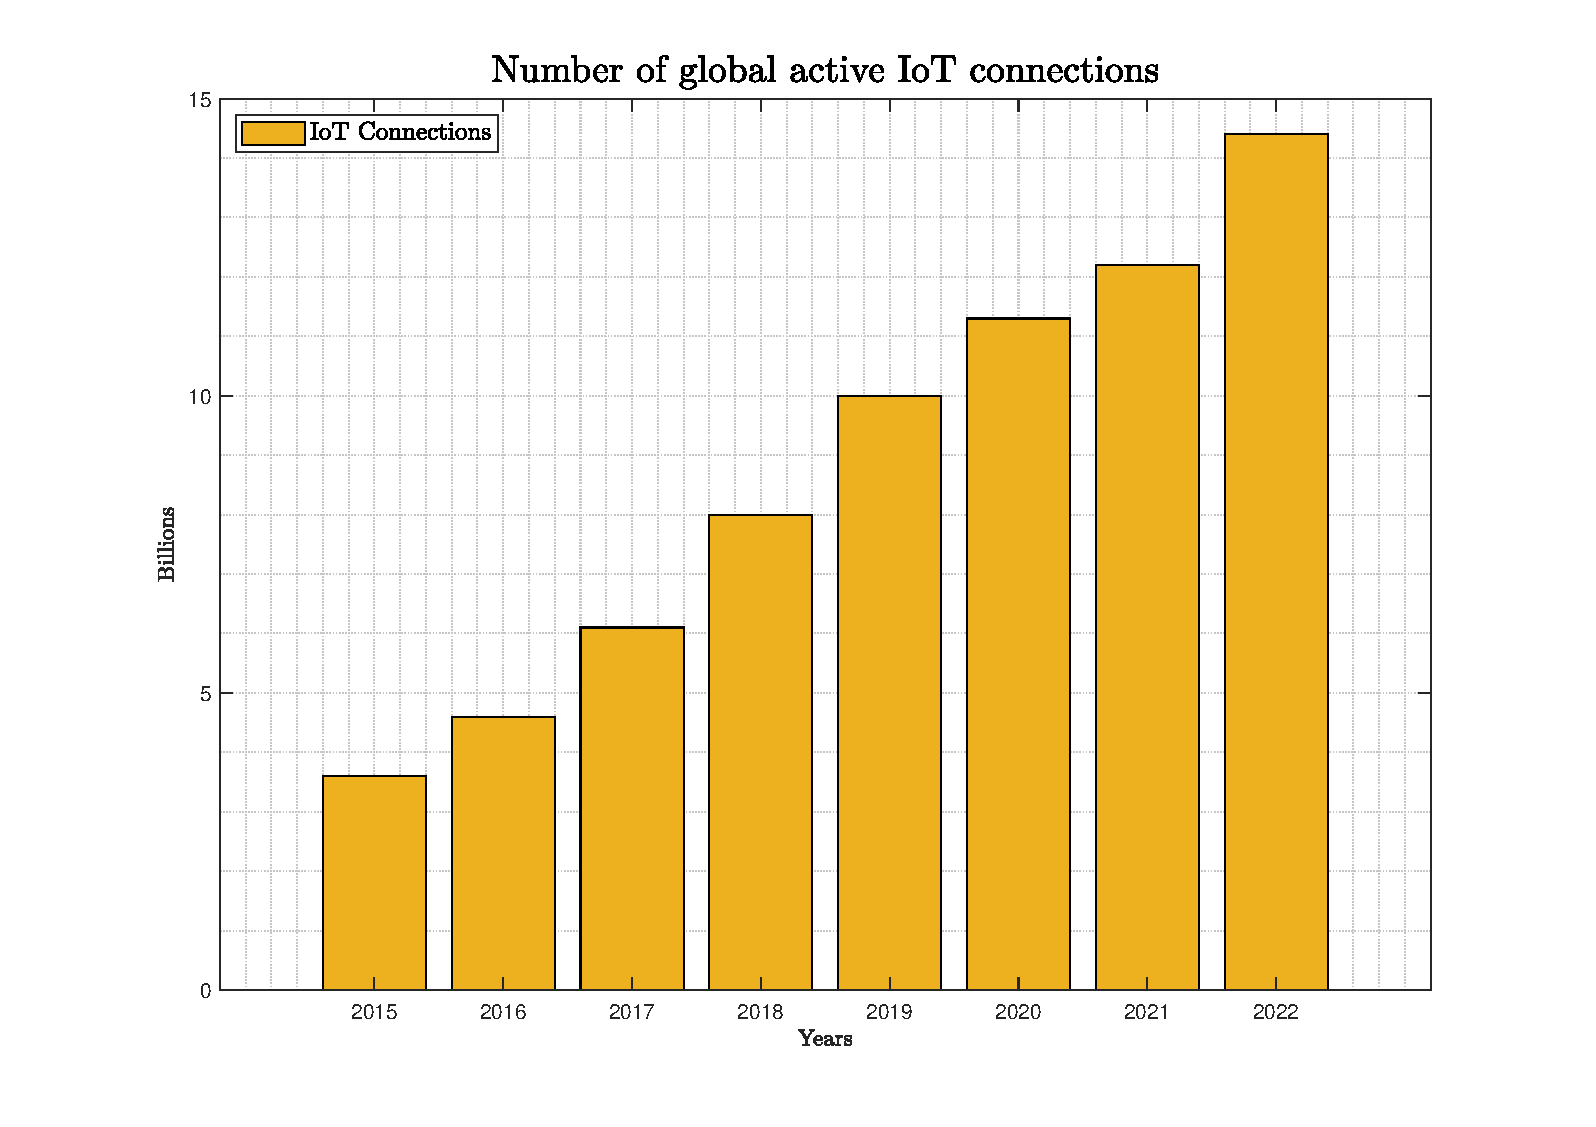
\includegraphics[width=\textwidth]{archivos/img/intro/fig_iot.eps}
    \caption{Estudio de las conexiones IoT máximas simultáneas a nivel global \cite{figuraIoTDevices}}
    \label{fig:intro_fig_iot}
\end{figure}

%6g
Por ello, se necesita una tecnología más avanzada que pueda satisfacer las futuras demandas de las redes \gls{iot}, y la tecnología \gls{6g} se postula como una solución a todos los nuevos retos planteados. Por esa razón, para facilitar el desarrollo de las futuras redes \gls{iot} la investigación en la siguiente generación de redes moviles ha recibido mucha atención tanto por parte de academia e instituciones, como por parte de la industria \cite{Nguyen2022}. \\
\\
Si bien es cierto que la tecnología \gls{6g} está todavía siendo formulada, se espera que esta pueda proporcionar una \gls{qos} totalmente mejorada frente a la generación anterior, dado sus prestaciones son claramente superiores, como por ejemplo, comuniaciones de ultabaja latencia, tasas de velocidad de datos mejoradas y entornos inteligentes de comunicación con satelites. \\
\\
Por consiguiente, muchos de los esfuerzos de las instituciones están pasando por impulsar las redes \gls{6g}-\gls{iot}. Desde Europa se está impulsando la carrera por el \gls{6g} poniendo sobre la mesa una hoja de ruta dividida en cuatro fases diferenciadas, esperando poder finalizar en 2030 \cite{eu6GFases}. Dichos esfuerzos están siendo coordinados desde la EU’s Smart Networks and Services Joint Undertaking (SNS-JU) la cual tiene como misiones principales impulsar el despliegue del \gls{5g}, y situar a los paises miembros de la EU a la vanguardía del desarrollo de la próxima generación de redes moviles \cite{eu6gSNS}. Estas misiones planean llevarlas a cabo a través de un detallado \textit{roadmap} el cual se puede apreciar en la figura \ref{fig:intro_banner_screen}.

\begin{figure}[ht]
    \centering
    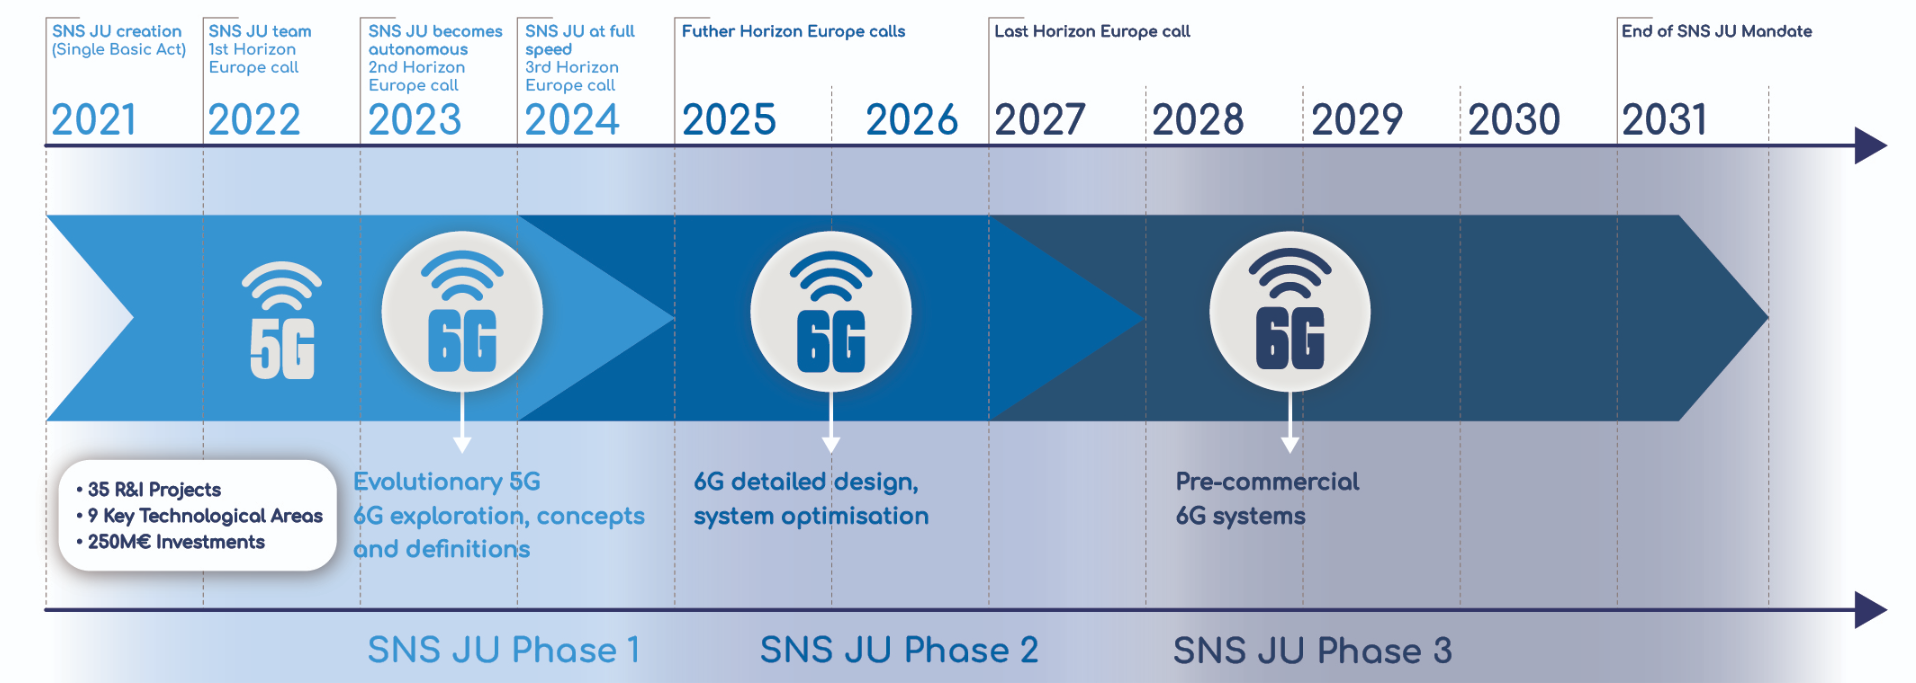
\includegraphics[width=\textwidth]{archivos/img/intro/banner-screen-1.png}
    \caption{\textit{Roadmap} propuesto por el SNS-JU para el desarrollo del \gls{6g} \cite{eu6gSNS}}
    \label{fig:intro_banner_screen}
\end{figure}


Dicho \textit{roadmap} se compone de varias fases, las cuales se han subdivido en streams. Los streams principales son cuatro, actualmente nos encontramos en el stream B del roadmap \cite{eu6GFase2}, el cual tiene como objetivo el impulso de la investigación en las areas tecnologicas habilitadoras del \gls{6g} además de la cooperación internacional con estados estrategicos como Estados Unidos. De entre todos los proyectos iniciados en 2023, destacan por ejemplo, Hexa-X~\cite{9482430}, iniciativa principal de europa liderada por Nokia financiado por el programa europeo Horizon 2020 que busca desarrollar el protipado de los sistemas \gls{6g}. Otro ejemplo, es el proyecto 6Genesis~\cite{Katz2019} financiado por Finlandia, que busca la generación de las primeras pruebas de concepto experimentales de redes \gls{6g}-\gls{iot}. Si nos vamos a proyectos más especificos, podemos encontrar ADROIT6G~\cite{ADROIT6G} y 6GTandem~\cite{6GTandem}, ambos han empezado en Enero de 2023 y buscan mejorar mejorar los sistemas distribuidos de acceso al medio mediante sistemas duales en frecuencia empleando procesado de señal \gls{mimo}.\\
\\
Pero el interés en la próxima generación de redes moviles, no es meramente local, si nos vamos a Estados Unidos, podemos ver como ya la FCC libera espectro en la banda de los THz en US para hacer pruebas de concepto para el 6G \cite{us6g}. O en a Corea del Sur, donde ya han pleando lanzar un proyecto piloto de \gls{6g} para el 2026 \cite{coreaSur6G}.\\
\\
Como se puede ver, el interés por el \gls{6g} es real, y se están realizando esfuerzos exhaustivos para la proliferación de las tecnologías habilitadoras del \gls{6g}, por lo que distintas instituciones apuntan a que las primeras redes \gls{6g} que podrán ser desplegadas en 2028 pero que su comercialización y la llegada a las personas de a pie no llegará hasta el 2030 \cite{Nguyen2022}.

https://hexa-x.eu/wp-content/uploads/2022/03/Hexa-X_D1.3.pdf
https://labs.etsi.org/rep/tfs/controller/-/tree/master/src/tests/ofc22
https://5g-ppp.eu/wp-content/uploads/2022/12/6G-Arch-Whitepaper_v1.0-final.pdf
https://ieeexplore.ieee.org/stamp/stamp.jsp?tp=&arnumber=9625032


\section{Redes \glsentryshort{sdn}}
\label{sec:6gIoT_sdn}


\section{Objetivos}
\label{sec:obj}

El objetivo principal de este proyecto es conseguir el desarrollo de un protocolo de control in-band eficiente
para la integración de la tecnologı́a IoT en las futuras de redes de 6G. Como ya hemos introducido, con la
llegada del IoT la dimensión de las redes va a crecer exponencialmente. Por lo consiguiente, la complejidad
de la administración de dichas redes va a suponer un gran desafı́o. Los dispositivos IoT se podrán beneficiar
de la integración con las redes SDN en 6G, ya que estas les reportará la flexibilidad y programabilidad
requerida para una correcta gestión y administración de cada elemento de la red. Por ello, se pueden resumir
los objetivos del proyecto en los siguientes puntos:

\begin{itemize}
    \item Analizar el estado del arte y necesidades actuales de IoT en 6G.
    \item Diseño de un protocolo in-band eficiente para IoT integrado con SDN.
    \item Emulación mediante plataformas como Contiki-NG, Mininet y ONOS.
    \item Implementación y despliegue en hardware real (tarjetas Raspberry Pi, o remotas IoT-LAB)
\end{itemize}





\section{Estructura del \glsentryshort{tfm}}
\label{sec:structure}



\section{Contribuciones}
\label{sec:contributions}


% Papers a meter
Este \gls*{tfm} ha proporcionado significativas contribuciones a la comunidad científica, incluyendo dos publicaciones en revistas de alto impacto indexadas en el JCR (2 Q2), un tercer trabajo en revisión (Q2). A continuación, se presentan estas contribuciones en resumen.\\
\\
Artículos de revistas científicas de alto impacto.

\begin{enumerate}
    \item Rojas, E., Hosseini, H., Gomez, C., \textbf{Carrascal, D.} and Cotrim, J.R., 2021. Outperforming RPL with scalable routing based on meaningful MAC addressing. Ad Hoc Networks, 114, p.102433. (JCR \textbf{Q2})
    \item Alvarez-Horcajo, J., Martinez-Yelmo, I., Rojas, E., Carral, J.A. and \textbf{Carrascal, D.}, 2022. ieHDDP: An Integrated Solution for Topology Discovery and Automatic In-Band Control Channel Establishment for Hybrid SDN Environments. Symmetry, 14(4), p.756. (JCR \textbf{Q2})
    \item \textbf{Carrascal, D.}, Rojas, E., Lopez-Pajares, D., Alvarez-Horcajo, J. and Carral, J.A., 2023. A Comprehensive Survey of In-Band Control in SDN:
          Challenges and Opportunities. Electronics, under review. (JCR \textbf{Q2})
\end{enumerate}

%El Internet de las Cosas (del inglés \textit{Internet of Things}, \gls{iot}) \cite{iotreview} y las Redes Definidas por Software (del inglés \textit{Software-Defined Networking}, \gls{sdn}) \cite{nadeau2013sdn}, son tecnologías emergentes que desde hace unos años están revolucionando los paradigmas sobre los modelos de redes comunicaciones establecidos en el pasado. \\
%\par

%Con las redes \gls{sdn}, como se puede apreciar en la figura \ref{sdnparadigma}, se desea extraer el plano de control de los dispositivos intermedios de procesamiento de la red, unificándolo en entes llamados controladores, haciendo la administración de red una tarea más centralizada y flexible. En cuanto al \gls{iot}, se pretende interconectar billones de objetos entre sí a través de Internet con la finalidad de que exista una comunicación máquina – máquina para proveer al usuario final de entornos inteligentes. 

% \begin{figure}[h]
%     \centering
%     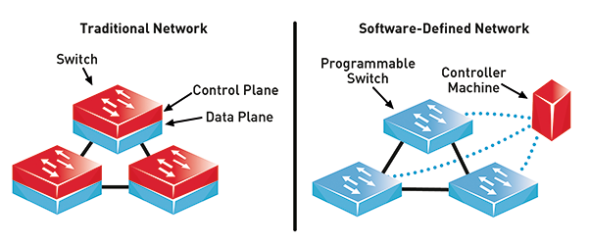
\includegraphics[width=6.5cm]{archivos/img/intro/sdn.png}
%     \caption{Paradigma en redes \glsentryshort{sdn}}
%     \label{sdnparadigma}
% \end{figure}

% Se considera como un punto de convergencia entre ambas tecnologías las redes 5G basadas fundamentalmente en \gls{sdn}, ya que prevén la incorporación de múltiples dispositivos \gls{iot}. Sin embargo, no todos los dispositivos \gls{iot} soportan una gestión basada en \gls{sdn} debido a las limitaciones que estos tienen en memoria, capacidad de procesamiento y  batería. Conforme el mundo de los dispositivos \gls{iot} avanza, las placas \gls{sbc} cada vez se hacen más potentes y de un tamaño más reducido, haciendo posible que éstas puedan ser incluidas como una pieza fundamental en proyectos \gls{iot} de alto rendimiento \cite{7501691}. \\

% \par

% Además, los sensores \gls{iot}, comúnmente conocidas como ``motas", continuamente se fabrican con más capacidad de procesamiento, memoria y batería con la finalidad de hacer frente a las nuevas redes de comunicaciones 5G \cite{capra2019edge}. Por todo ello,  se estima que la integración con las redes \gls{sdn} está cada vez más próxima. Generalmente, se están siguiendo estas vías de actuación:
% \begin{itemize}
%     \item \label{iot_integracionParcial}Realizar una integración parcial, haciendo uso de de dispositivos mediadores entre las motas y el core \gls{sdn}. Este dispositivo mediador, sería un dispositivo híbrido con interfaces inalámbricas y alámbricas para tener de acceso a la red \gls{sdn} \cite{7848825}.

%           \begin{figure}[h]
%               \centering
%               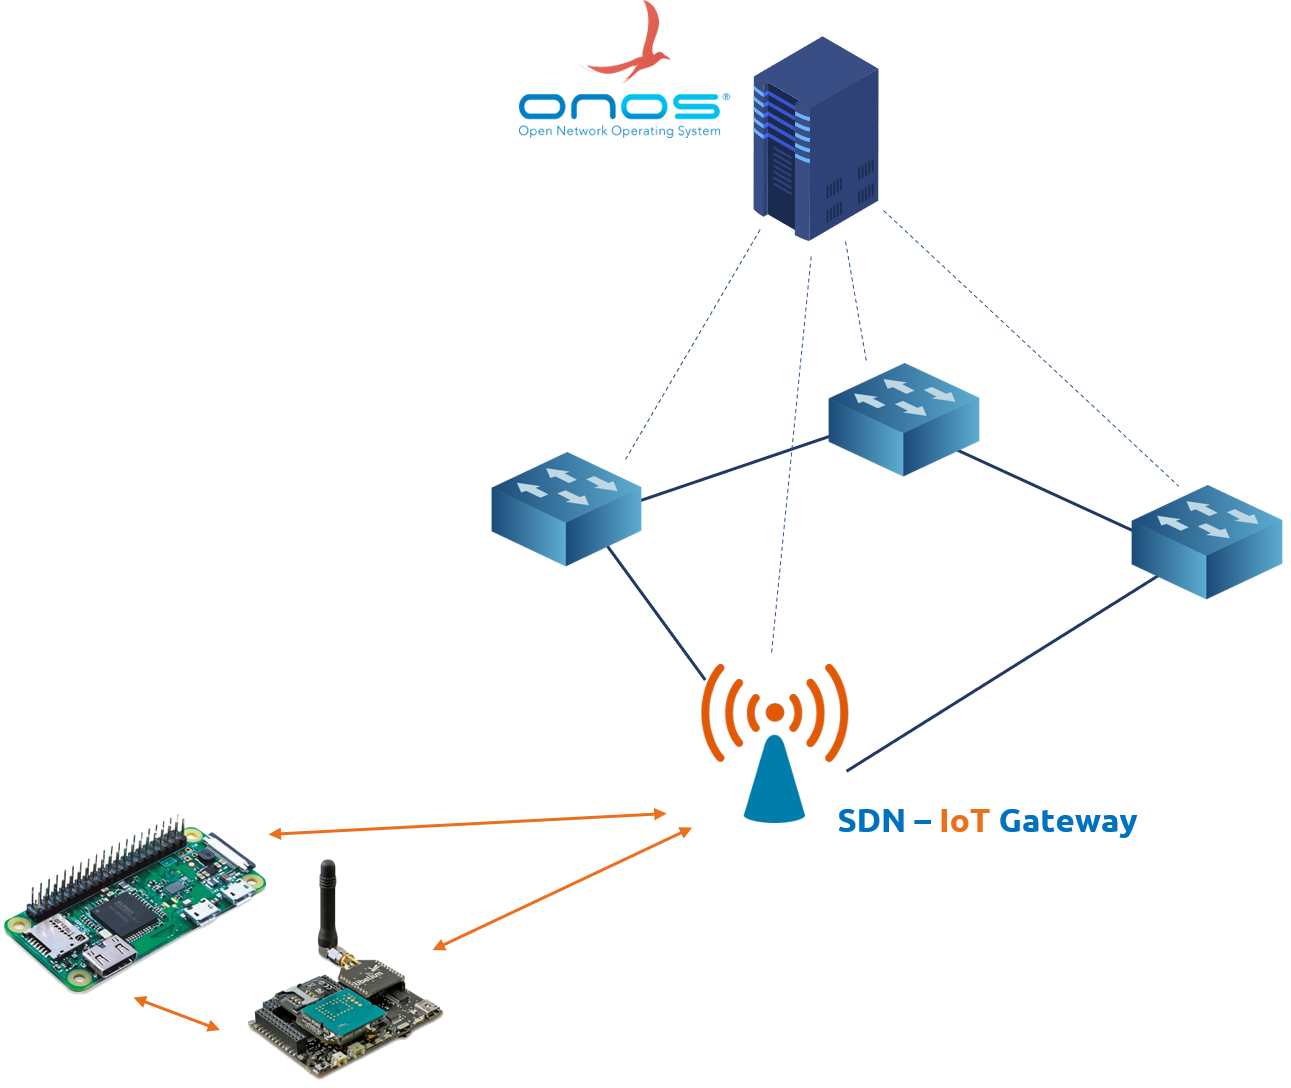
\includegraphics[width=10cm]{archivos/img/intro/sdn_iot.png}
%               \caption{Integración parcial de dispositivos \glsentryshort{iot} en el core \glsentryshort{sdn}}
%               \label{sdn_iot_parcial}
%           \end{figure}
%           Como se puede ver en la figura \ref{sdn_iot_parcial}, haciendo uso de un dispositivo mediador, este actuaría de pasarela o \textit{gateway} para las redes de sensores. De esta manera, se delega toda la carga de procesamiento y consumo de batería que supone integrar la interfaz de control \gls{sdn}. Además, se implementarían los distintos protocolos y estándares para comunicarse con los dispositivos \gls{iot}. Esta vía también ofrece otros aspectos positivos, entre los cuales se puede destacar, emplear el gateway como un traductor de protocolos \gls{iot} \cite{8470257}. Esto permitiría que distintos sensores que tuvieran implementados diferentes protocolos como, por ejemplo, \gls{ble}\footnote{Especificación del protocolo:  \url{https://www.bluetooth.com/specifications/}} y Zigbee\footnote{Protocolo de alto nivel basado en el estandar \gls{ieee} 802.15.4, especificación: \url{https://zigbeealliance.org/solution/zigbee/} }, pudieran interactuar entre sí a través del  gateway \gls{iot}.

%     \item \label{iot_integracionTotal}Realizar una integración total, como se puede apreciar en la figura \ref{sdn_iot_total}, donde el propio dispositivo \gls{iot} es capaz de co-existir en la red \gls{sdn}. Esta última vía es la más ambiciosa debido a que se requiere de hardware lo suficientemente potente para soportar la lógica \gls{sdn}, y de una tecnología que establezca su plano de datos de forma más eficiente posible para optimizar al máximo los recursos limitados del dispositivo.

%           \begin{figure}[ht]
%               \centering
%               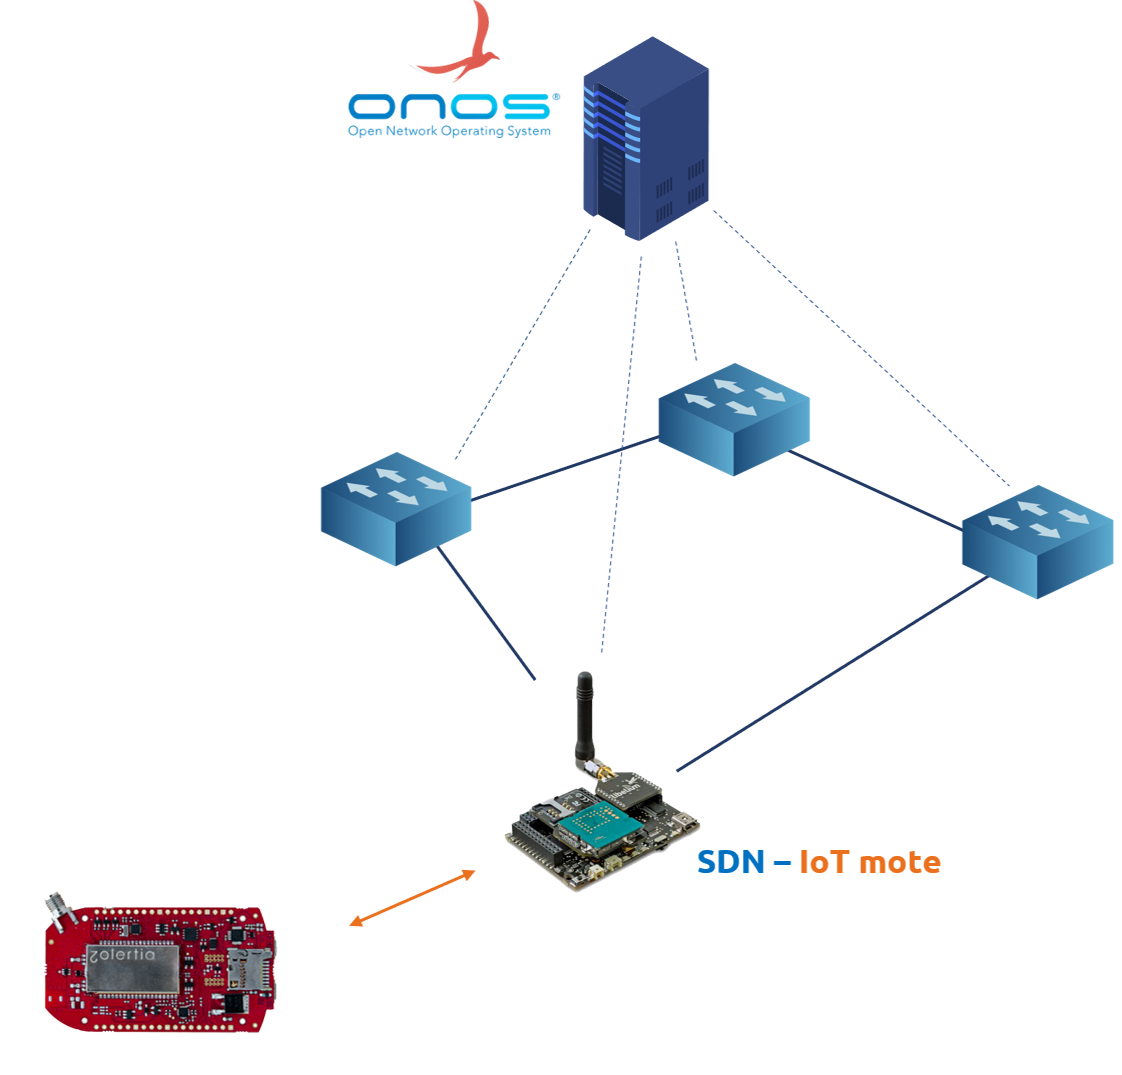
\includegraphics[width=10cm]{archivos/img/intro/sdn_iot_b.png}
%               \caption{Integración total de dispositivos \glsentryshort{iot} en el core \glsentryshort{sdn}}
%               \label{sdn_iot_total}
%           \end{figure}

% \end{itemize}



% \section{Tecnologías para la definición del datapath}



% En redes convencionales previas al concepto de \gls{sdn}, los nodos de la red tenían unificado un plano de control, \textit{Control plane}, donde se definía la lógica que dictaba como debía llevarse a cabo el \textit{forwarding} de los paquetes, y un plano de datos, \textit{Data plane}, el cual se puede implementar definiendo su datapath. Dicho datapath se compone de varios bloques de procesado para reenviar los paquetes. Con la llegada del paradigma de las redes \gls{sdn}, como se puede apreciar en la figura \ref{sdnparadigma}, los nodos clásicos de red verían como su plano de control sería delegado a una entidad llamada controlador. El controlador tendría una perspectiva global de toda la red en su conjunto pudiendo gestionarla de una manera más flexible y centralizada. \\
% \par
% En consecuencia, los nodos de la red estarían destinados a implementar un plano de datos, y una interfaz de control para ser configurados por el controlador mediante protocolos como, por ejemplo, OpenFlow\footnote{\url{https://www.opennetworking.org/software-defined-standards/specifications/}}. \\
% \par
% Por lo tanto, para ejecutar la integración de los dispositivos \gls{iot} en las redes \gls{sdn} se debe poder definir un datapath en dichos dispositivos y que estos posean una interfaz de control para ser configurados desde un hipotético controlador. Debido a esto, se requiere hacer uso de tecnologías que nos permitan definir el plano de datos de estos dispositivos. En este \gls{tfg}, se abordarán las siguientes tecnologías:

% \begin{itemize}
%     \item El lenguaje \textbf{P4}. Este lenguaje de alto nivel nos permite definir el procesado de los paquetes para un conjunto de arquitecturas. Dichas arquitecturas tienen su propia especificación. Con ello, se quiere conseguir que los programas P4 sean independientes del \textit{hardware} donde se ejecute \cite{2014p4}.

%     \item \textbf{\gls{xdp}}. Es un \textit{framework} programable y de alto rendimiento para el procesado de paquetes en el Kernel de Linux. El procesado de los paquetes se lleva a cabo en el punto más bajo de la pila de red de Linux, consiguiendo así añadir nuevas funcionalidades sin necesidad de modificar el propio Kernel. Además, el hecho de definir el procesado de paquetes casi en la propia interfaz, reporta un gran rendimiento ya que no es necesario atravesar toda la pila de protocolos, con todo lo que eso conlleva (reservas de memoria, reservas de memoria para metadatos, encolado de los paquetes, desencapsulado de cabeceras, análisis y tratamiento de cabeceras, etc) \cite{xdp1}.
% \end{itemize}



% \section{Objetivos}

% El objetivo de este proyecto es realizar un estudio y análisis de las tecnologías P4 y \gls{xdp} para la integración de dispositivos \gls{iot} en entornos \gls{sdn}. Como ya hemos introducido, con la llegada del \gls{iot}, la dimensión de las redes va a crecer exponencialmente. Por consiguiente, la complejidad de la administración de dichas redes va a suponer un gran desafío.  Los dispositivos \gls{iot} se podrán beneficiar de la integración con las redes \gls{sdn}, ya que éstas les reportarán la \textbf{flexibilidad} y \textbf{programabilidad} requerida para una correcta gestión y administración de cada elemento de la red. Para alcanzar dicho objetivo, se han planteado los siguientes puntos:

% \begin{itemize}
%     \item \textbf{Documentación y estudio}: Búsqueda y recolección de información, artículos y guías para tener
%           los conocimientos básicos necesarios sobre el estado del arte actual y de las tecnologías para definir el plano de datos. De esta forma, se podrá plantear los diseños y desarrollos más optimizados, de cara a favorecer las limitaciones impuestas por los dispositivos \gls{iot}.

%     \item \textbf{Planteamiento de casos de uso típicos y elección de escenarios}: Se hará un planteamiento de funcionalidades básicas, casos de uso, que una tecnología que define un datapath debe ser capaz de proveer. Además, se elegirán los escenarios y plataformas para desplegar dichos casos de uso.

%     \item  \textbf{Desarrollo de los casos de uso}: Se abordará el desarrollo de dichos casos de uso con ambas tecnologías (P4, \gls{xdp}) en los escenarios planteados. Se tratará que los escenarios donde se desplieguen los desarrollos sean lo más homogéneos posibles, para que los puntos fuertes y débiles de cada tecnología puedan ser esclarecidos.

%     \item \textbf{Evaluación y comprobación de funcionamiento}: Se comprobará el correcto funcionamiento de todos los casos de uso desarrollados y por último, se evaluará que tecnología es más idónea para definir el datapath de los dispositivos \gls{iot} en su integración en entornos \gls{sdn}.
% \end{itemize}


% \section{Estructura del \glsentryshort{tfg}}

% En esta sección se indica la estructura básica de este \gls{tfg}, haciendo un breve resumen de los aspectos más importantes y significativos de cada capítulo.


% \begin{description}
%     \item\textbf{Capítulo 1: Introducción}. Se hará una breve introducción de la motivación que ha originado la realización de este \gls{tfg}, así como una breve explicación de los aspectos generales y de los objetivos que se quieren alcanzar con el trabajo presentado.

%     \item\textbf{Capítulo 2: Estado del arte}. Se documentarán conceptos fundamentales en relación al proyecto, además de todas las diferentes herramientas que sean utilizadas. La motivación de este capítulo es la de establecer un marco teórico lo suficientemente consistente para abordar el análisis y el diseño de forma óptima, previo al desarrollo.

%     \item\textbf{Capítulo 3: Diseño y análisis de casos de uso}. Se debatirá y analizará que funcionalidades básicas deben tener las distintas tecnologías para definir el datapath. Para ello, se diseñarán distintos casos de uso para así demostrar la eficiencia de una tecnología sobre la otra en la integración de los dispositivos \gls{iot} en entornos \gls{sdn}.

%     \item\textbf{Capítulo 4: Desarrollo y evaluación de casos de uso}. Se describirá el desarrollo realizado, indicando las partes más importantes de cada caso de uso, ofreciendo al final de cada caso una evaluación de su funcionamiento.

%     \item\textbf{Capítulo 5: Conclusiones y trabajo futuro}. Se terminará la memoria con las conclusiones del trabajo realizado, y se presentarán las vías de trabajo futuro que tiene este proyecto.

%     \item[]\textbf{Bibliografía y referencias}. Se añadirán todos los artículos, libros, materiales consultados y empleados en la elaboración de esta memoria. Se seguirá el estilo de citación del \gls{ieee}, siguiendo las recomendaciones oficiales de la normativa sobre \gls{tfg}s de la \gls{uah}.

%     \item[]\textbf{Anexos}. Se incluirán todos los manuales de usuario e instalación que se consideren oportunos. De forma adicional, se añadirán las características técnicas del \textit{hardware} con el cual se ha desarrollado este \glsentryshort{tfg}. Por último, se hará un presupuesto que incluya el coste de mano de obra, material y gastos generales.

% \end{description}

%%%%%%%%%%%%%%%%%%%%%%%%%%%%%%%%%%%%%%%%%%%%%%%%%%%%%%%%%%%%%%%%%%%%%%%%%%%%%%%%%%%%%%%%%%%%%%%%%%%%
%\chapter{Estado del arte}
\label{estadoArte}

En el presente capítulo se describirán los conceptos fundamentales relacionados con el proyecto, así como las diversas herramientas que se utilizarán mayoritariamente. El propósito de este capítulo es establecer un marco teórico sólido que permita abordar el análisis y el diseño del protocolo de comunicación \textit{in-band} de manera óptima antes de su desarrollo. Finalmente, se hará referencia a las contribuciones y la documentación generada con el fin de difundir los contenidos del proyecto a través de la plataforma \textit{GitHub}.


%%%%%%%%%%%%%%%%%%%%%%%%%%%%%%%%%%%%%%%%%%%%%%%%%%%%%%%%%%%%%%%%%%%%%%%%%%%%%%%%%%%%%%%%%%%%%%%%%%%%%
% 6G
%%%%%%%%%%%%%%%%%%%%%%%%%%%%%%%%%%%%%%%%%%%%%%%%%%%%%%%%%%%%%%%%%%
\section{Red de comunicación \glsentryshort{6g}}
\label{sec:6g}

%%%%%%%%%%%%%%%%%%%%%%%%%%%%%%%%%%%%%%%%%%%%%%%%%%%%%%%%%%%%%%%%%%%%%%%%%%%%%%%%%%%%%%%%%%%%%%%%%%%%%
% IoT
\section{Tecnología \glsentryshort{iot}}
\label{iot}

La premisa básica de la tecnología \gls{iot} \cite{iotreview} conectar cualquier dispositivo que tenga cierta capacidad de cómputo. Esto significa que los objetos que actualmente no están conectados a Internet, estarán conectados de manera que puedan comunicarse e interactuar con personas y otros objetos. \\
\par

La tecnología \gls{iot} es una transición tecnológica en la que los dispositivos al ser dotados de inteligencia por estar conectados a Internet podrán proveer de entornos inteligentes a los humanos.  Cuando los objetos puedan ser controlados a distancia a través de una red, se habilitará una integración más estrecha entre el mundo físico y las máquinas, permitiendo mejoras en las áreas de medicina, automatización y logística \cite{7073822}.\\
\par

El ecosistema \gls{iot} es amplio, e incluso se puede parecer un poco caótico debido a la gran cantidad de componentes y protocolos que abarca. Es recomendable en vez de ver el \gls{iot} como un termino único, verlo como un paraguas de varios conceptos, protocolos y tecnologías, enfocados a un mismo propósito de interconectar ``Cosas" a Internet. Si bien la amplia mayoría de elementos \gls{iot} están diseñados para aportar numerosos beneficios en las áreas de productividad y automatización, al mismo tiempo introducen nuevos desafíos, como por ejemplo la gestión de la gran cantidad de dispositivos que van a aparecer en las redes, y la cantidad de datos y mensajes que todos estos generaran \cite{iotreview}.

\subsection{Arquitectura}

Aunque en el ecosistema hay diferentes \textit{stacks} de protocolos, todos ellos se pueden resumir en la siguiente arquitectura básica \cite{iotreview}.

\begin{itemize}
    \item \textit{Perception Layer}, en esta capa se da un significado físico a cada objeto. Consiste en sensores de diferentes tipos como etiquetas RFID, sensores IR u otras redes de sensores que podrían detectar la temperatura, la humedad, la velocidad y la ubicación, etc. Esta capa recolecta información útil a partir de los sensores vinculados a los objetos,  convierte dicha información en señales digitales que más tarde se delegarán a la Capa de Red para su posterior transmisión.
    
    \item \textit{Network Layer}, el propósito de esta capa es la de recibir la información en
    forma de señales digitales desde la capa de Percepción y transmitirla a los sistemas de procesamiento en la capa de \textit{Middleware}. Esto se llevará a cabo a través de las distintas tecnologías de acceso como WiFi, BLE, WiMaX, ieee802154 y con protocolos como IPv4, IPv6, MQTT.
    
    \item \textit{Middlware Layer}, en esta capa se procesa la información recibida de todos los sensores. En esta capa se puede incluir las tecnologías como Cloud computing, o sistemas gestores,  que aseguran un acceso directo a bases de datos donde se puede almacenar toda la información recolectada. Teniendo una gran cantidad de información centralizada, generalmente se aplican sistemas de inteligencia artificial para procesar la información, y tomar decisiones predictivas totalmente automatizadas. Estos sistemas suelen ser utilizados para analizar el tiempo, contaminación o tráfico en las ciudades. 
    
    \item \textit{Application Layer}, la finalidad de  esta  capa es la de realizar las aplicaciones \gls{iot} para el usuario final. Estas aplicaciones se valdrán de los datos procesados para ofrecer funcionalidades al usuario final, por ejemplo, una aplicación del tiempo.
    
    \item \textit{Business Layer}, esta capa aunque es un poco abstracta, se suele añadir para representar la gestión de múltiples las aplicaciones y servicios \gls{iot}. 
\end{itemize}

% Foto 
\begin{figure}[ht]
    \centering
    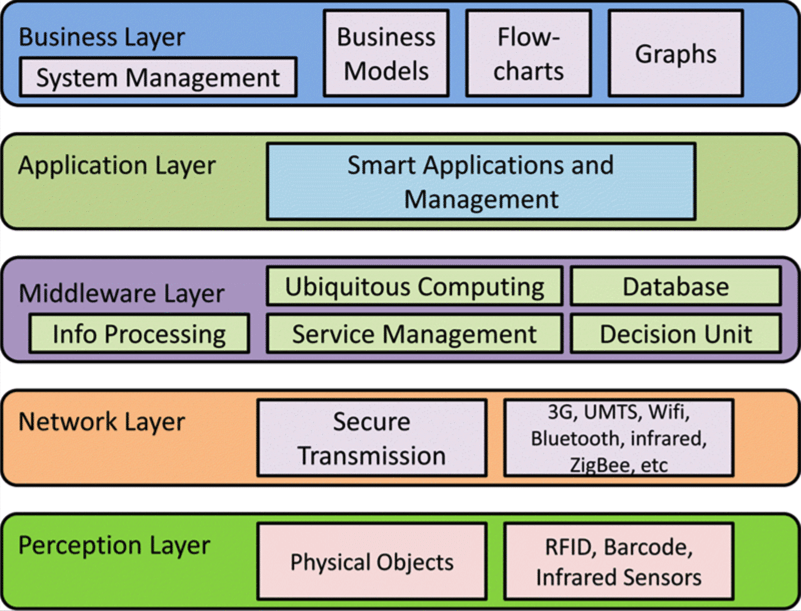
\includegraphics[width=6.5cm]{archivos/img/teoria/arch_edited.png}
    \caption{Arquitectura básica \glsentryshort{iot}}
    \label{fig:iotBasicArch}
\end{figure}

\subsection{Topologías}

Entre las tecnologías de acceso disponibles para conectar los dispositivos de \gls{iot}, dominan tres esquemas topológicos principales, estrella, malla y p2p. Para las tecnologías de acceso de largo y corto alcance, predomina la topología de estrella, como se puede encontrar en las redes datos móviles, LoRa y BLE. Las topologías en estrella utilizan una única estación base central para permitir las comunicaciones con los nodos finales. En cuanto a las tecnologías de mediano alcance, se pueden encontrar topologías en estrella, de p2p o en malla, como se ve en la figura \ref{fig:iotTopo}. Generalmente se suele hacer uso de un tipo de topología sobre otra en función de las limitaciones de los nodos que la conforman \cite{iotbook}.\\
\par

% Foto 
\begin{figure}[ht]
    \centering
    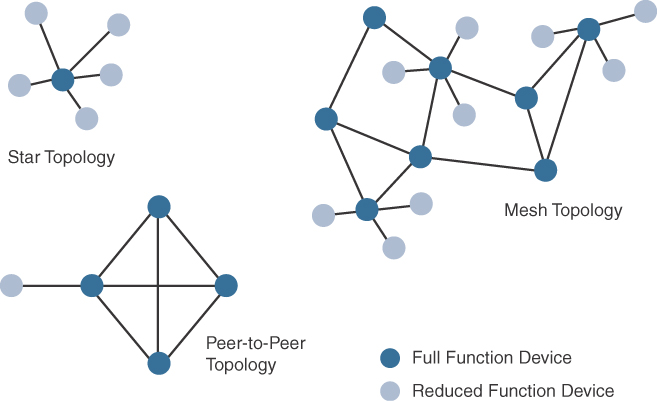
\includegraphics[width=7.5cm]{archivos/img/teoria/iot_topo.jpg}
    \caption{Tipos de topología con dispositivos \glsentryshort{iot} \cite{iotbook}}
    \label{fig:iotTopo}
\end{figure}


\subsection{Redes LLN}

Las redes de baja capacidad, conocidas como, \gls{lln}\footnote{\url{https://tools.ietf.org/html/rfc7228}}, se caracterizan por estar compuestas de dispositivos (sensores, motas) con limitaciones de memoria, batería y procesamiento. Dichos nodos, se interconectarán haciendo uso de distintos de tipos de enlace, como por ejemplo \texttt{ieee802154} ó LowPower-WiFi \cite{llnrfc}. Este tipo de redes pueden estar presentes en distintos campos de aplicación, entre las que se incluyen asistencia sanitaria, monitorización industrial, redes de sensores, etc.   \\

\par
Otra condición de las redes \gls{lln}, son las pérdidas en capa física debidas a las interferencias y variabilidad de los ``complicados" entornos radio donde estarán desplegadas dichas redes. Por ello, y teniendo en cuenta que los nodos que formarán parte de las redes \gls{lln} serán de baja capacidad, es necesario que los protocolos utilizados en esta red sean capaces de optimizar al máximo los recursos de los dispositivos \cite{iotbook}. 

\subsubsection{IEEE 802.15.4}

El estándar \texttt{ieee802154}\footnote{\url{https://tools.ietf.org/id/draft-ietf-lwig-terminology-05.html}} define la tecnología acceso a un entorno inalámbrico (\textit{phy} y \textit{mac}) para dispositivos de baja capacidad (limitados en batería y capacidad de transmisión). Este estándar se caracteriza por la optimización de los recursos del nodo en cuestión, consiguiendo una duración prolongada de la batería, además, esta tecnología de acceso permite un fácil uso utilizando un \textit{stack} de protocolos compacto, al tiempo que sigue siendo simple y flexible. Por todas estas características, el estándar \texttt{ieee802154} es usado en la mayoría de \textit{stack} de protocolos enfocados al \gls{iot}. Uno de los más utilizados es el \textit{stack} 6LoWPAN, definido por el \gls{ietf}, consiste en una capa de adaptación de IPv6 sobre las capas del estándar \texttt{ieee802154} (Ver figura \ref{fig:6lowapan}) \cite{6lowpan}.\\
\par

\vspace{0.5cm}

% Foto 
\begin{figure}[ht]
    \centering
    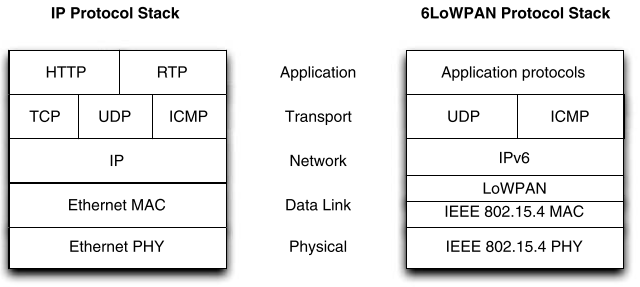
\includegraphics[width=12cm]{archivos/img/teoria/6LoWPAN-Protocol-Stack.png}
    \caption{Pila de protocolos 6LoWPAN \cite{6lowpan}}
    \label{fig:6lowapan}
\end{figure}



%%%%%%%%%%%%%%%%%%%%%%%%%%%%%%%%%%%%%%%%%%%%%%%%%%%%%%%%%%%%%%%%%%%%%%%%%%%%%%%%%%%%%%%%%%%%%%%%%%%%%
% SDN
\section{Redes  \glsentryshort{sdn}}
\label{sec:sdn}


El paradigma \gls{sdn} \cite{nadeau2013sdn} consiste en una arquitectura de red donde se lleva a cabo la separación del plano de control de la red para centralizarlo en un único ente llamado controlador. De esta forma se consigue que la administración de red sea una tarea más centralizada y flexible \cite{nadeau2013sdn}. La idea del \gls{sdn} empezó a germinar en la Universidad de Stanford por el año 2003, donde el profesor asociado en su momento, Nick McKeown, planteaba las limitaciones de las redes convencionales y veía la necesidad de replantear como los \textit{backbones} debían operar \cite{sdnBegins}. Dicha idea se acuñó como \gls{sdn} en el año 2011, cuando a la par se lanzó la organización \gls{onf} \cite{onf} como un portador de los estándares relacionados con el \gls{sdn} y su difusión.

\subsection{Arquitectura}

La arquitectura \gls{sdn} destaca por ser dinámica, rentable y adaptable haciéndola ideal para las demandas presentadas hoy en día por las redes de comunicaciones. Como ya se ha comentado, la arquitectura se basa en separar el plano de control del plano de datos, y llevar ese plano de control a una entidad llamada controlador. Desde dicha entidad se ofrecerán las interfaces necesarias para que aplicaciones de servicios de red puedan hacer uso de ellas. De esta forma, el control de la red se vuelve directamente programable, consiguiendo que la gestión se vuelva más ágil y dinámica.\\
\par

Como se puede ver en la figura \ref{fig:sdnBasicArch}, la arquitectura \gls{sdn} se divide en tres capas, la primera, el plano de datos que contendrá todos los elementos de red que habiliten el forwarding. La segunda, el plano de control, compuesto de los distintos controladores de la red \gls{sdn}, y por último, la capa de aplicación, en la cual se encontrarán todas las aplicaciones que se comuniquen con el controlador \gls{sdn}. \\
\par
Dichas capas se comunicarán entre ellas a través de interfaces abiertas. Por ejemplo, la interfaz \textit{Southbound} permite programar el estado de reenvío de los elementos de red del plano de datos. En cambio, la interfaz \textit{Northbound} comunica las aplicaciones con los controladores \gls{sdn}, habilitando la obtención de datos o el ajuste de parámetros a través de una API-Rest. También se pueden encontrar otro tipo de interfaces, \textit{Westbound} y \textit{Eastbound}, que se han consolidado los últimos años para la interconexión de controladores con la finalidad de establecer una misma política entre distintos dominios \gls{sdn}.

% Foto 
\begin{figure}[ht]
    \centering
    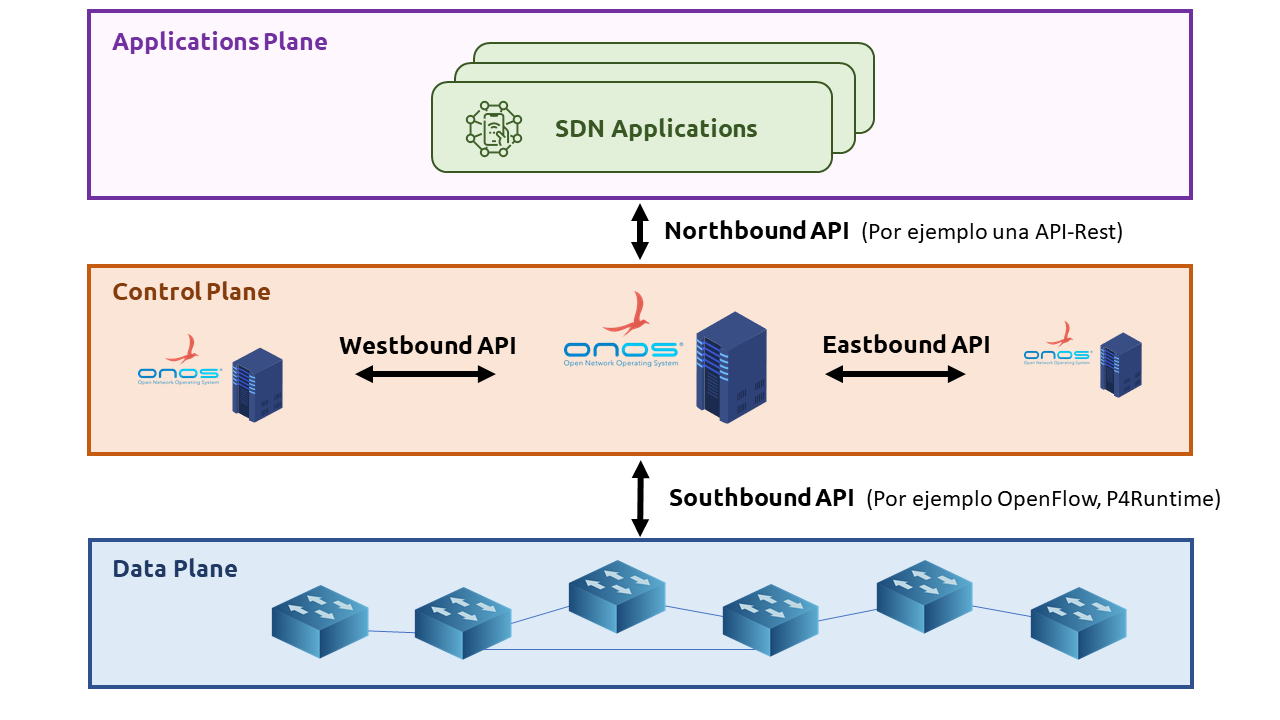
\includegraphics[width=14.5cm]{archivos/img/teoria/sdn_arch.png}
    \caption{Arquitectura básica \glsentryshort{sdn}}
    \label{fig:sdnBasicArch}
\end{figure}

\subsection{OpenFlow}

Existen varios protocolos para el control de los elementos de red desde el controlador, pero el más utilizado es Openflow. OpenFlow es un protocolo de la interfaz \textit{Southbound} que comunica los controladores \gls{sdn} con los elementos de red para configurar el estado de reenvío de estos últimos. La especificación de este protocolo se encuentra recogida por la \gls{onf}\footnote{\url{https://www.opennetworking.org/software-defined-standards/specifications/}}, contando con numerosas versiones siendo la última la versión \texttt{1.5.1} del 2015. \\
\par

El elemento clave de OpenFlow es el flujo (\textit{flow}), los cuales se conforman de paquetes que ha sido clasificados en función de reglas. Dichas reglas se encuentran en las tablas de flujo (\textit{flow table}) y  suelen estar relacionadas con los puertos de entrada o valores de cabecera típicos. Cuando estos criterios coinciden con los del paquete entrante se produce un \textbf{\textit{match}}.\\
\par
En el momento en que se produce un \textit{match}, el paquete en cuestión se verá sujeto a una serie de instrucciones asociadas a la regla con la que a hecho \textit{matching}. Estas instrucciones pueden ir desde, hacer una medición del paquete, aplicar una acción ó ir a otra tabla de flujo. De esta forma, con unas tablas de flujo completadas con unas reglas suministradas por el controlador \gls{sdn}, se conforma el estado de reenvío del switch en cuestión \cite{nadeau2013sdn}. 


%%%%%%%%%%%%%%%%%%%%%%%%%%%%%%%%%%%%%%%%%%%%%%%%%%%%%%%%%%%%%%%%%%%%%%%%%%%%%%%%%%%%%%%%%%%%%%%%%%%%%
% Linux Networking
\section{Linux Networking}
\label{sec:linuxNetworking}

Esta sección recopilará todos los conceptos y herramientas relacionadas con la parte de Networking en Linux, que son fundamentales para el desarrollo, análisis y validación de este proyecto.


%%%%%%%%%%%%%%%%%%%%%%%%%%%%%%%%%%%%%%%%%%%%%%%%%%%%%%%%%%%%%%%%%%%%%%%%%%%%%%%%%%%%%%%%%%

\subsection{Interfaz virtual - \texttt{tun/tap}}
\label{linuxNetworking_tuntap}

En el mundo de las redes siempre se habla de las interfaces tun/tap de forma indistinta cuando van a utilizarse, sin embargo, cada una tiene su cometido. Como se ha indicado, en networking, las interfaces TUN y TAP son interfaces virtuales que se crean y se gestionan en espacio de kernel. Mencionar que como estas interfaces son virtuales y se gestionan directamente vía softaware, no como las interfaces reales que se gestionan con unos drivers diferentes, cada interfaz con su driver específico de la interfaz.  Los drivers de las interfaces TUN/TAP se crearon en los 2000 como una unión de los avances de los drivers desarrollados en las comunidades de Solaris, Linux, BSD. Actualmente los drivers solo tienen mantenimiento por los kernels de linux y FreeBSD. Ambos tipos de interfaces se utilizan para tunelado, pero no pueden ser utilizadas a la vez dado que trabajan en niveles distintos. Las TUN, de \textit{network \textbf{TUN}nel}, emula la capa de red y puede llegar hacer reenvío de los paquetes. En cambio las interfaces TAP,  trabajan en capa 2 solo en capa dos, y emulan un equipo que trabaja en dicha capa, como por ejemplo un switch. Por tanto, hay que dejar claro lo que se puede llegar a realizar con cada interfaz (Ver figura \ref{fig:linux1}).

\begin{itemize}
    \item \texttt{TUN} se puede llegar a utilizar para routing.
    \item \texttt{TAP} se puede llegara utilizar para crear un bridge.
\end{itemize}

Generalmente, cuando los paquetes son enviados por el sistema operativo a través de una interfaz TUN/TAP,  serán recibidos por algún programa de espacio de usuario, el cual, está enganchado directamente en la interfaz. Cualquier programa de espacio de usuario podrá pasar paquetes por las interfaces, y las interfaces virtuales se lo pasarán al \textit{stack} de red por defecto, emulando la recepción de los paquetes inyectados desde espacio de usuario.

% fig
\begin{figure}[ht]
    \centering
    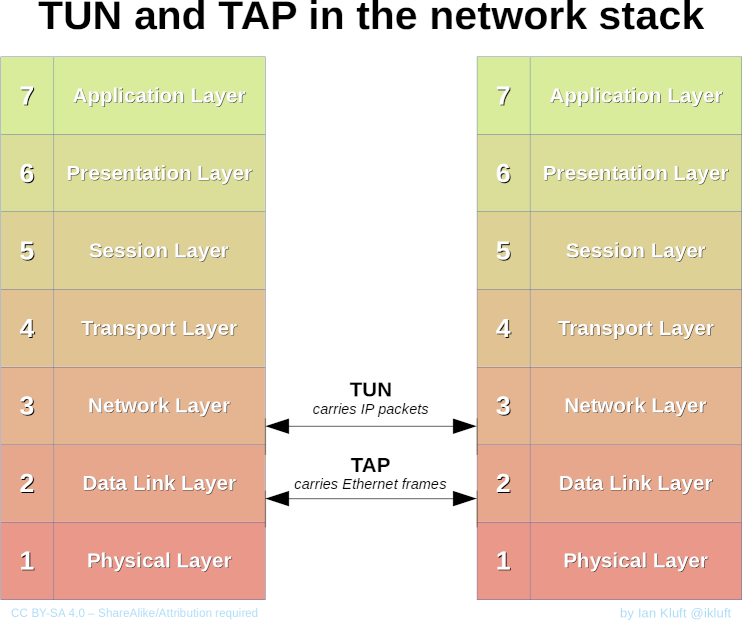
\includegraphics[width=\textwidth]{archivos/img/teoria/linux1.png}
    \caption{Diagrama de funcionamiento de las interfaces virtuales TUN/TAP }
    \label{fig:linux1}
\end{figure}

Para la creación de estas interfaces lo podemos hacer por ioctl o podemos hacerlo más fácil a través del binario tunctl o en su defecto con el comando de \texttt{tuntap} del set de herramientas iproute2. A continuación, en el bloque \ref{code:tun_tap_use} se indican todos los comandos necesarios para trabajar con las interfaces TUN/TAP.

\begin{lstlisting}[language= bash, style=Consola, caption={Manejo de interfaces TUN - TAP},label=code:tun_tap_use]
    # En caso de querer utilizar tunctl hay que instalar el binario
    sudo apt install -y uml-utilities
    
    # Para crear una un interfaz podemos hacer lo siguiente
    tunctl -t {nombre_tun}

    # Para eliminarla
    tunctl -d {nombre_tun}

    # Para crear interfaces de tipo TAP hay que hacer lo siguiente
    tunctl -p -t {nombre_tun}
    
    # El comando análogo con iproute2 sería el siguiente
    ip tuntap add dev {nombre_tun} mode {tun|tap}
\end{lstlisting}
\vspace{0.5cm}

En caso de que queramos comprobar que las interfaces se han creado correctamente siempre se puede hacer uso de la herramienta \texttt{ethtool}. A continuación, en la figura \ref{fig:linux2}, se puede ver como en el campo \texttt{bus-info} nos indica que tipo de interfaz es.

% fig
\begin{figure}[ht]
    \centering
    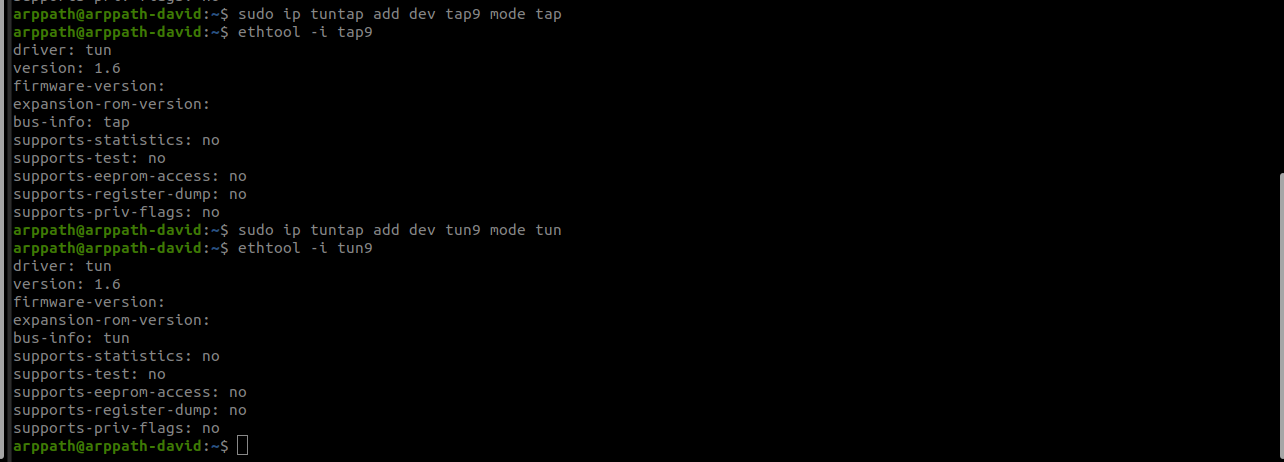
\includegraphics[width=\textwidth]{archivos/img/teoria/linux2.png}
    \caption{Comprobación con \texttt{ethtool} de tipo de interfaz virtual.}
    \label{fig:linux2}
\end{figure}


%%%%%%%%%%%%%%%%%%%%%%%%%%%%%%%%%%%%%%%%%%%%%%%%%%%%%%%%%%%%%%%%%%%%%%%%%%%%%%%%%%%%%%%%%%
\subsection{Interfaz virtual - \texttt{veth}}
\label{linuxVeths}
Las \gls{veth}, son interfaces de Ethernet virtuales creadas como un par de interfaces interconectadas entre si. El modelo funcional es sencillo, los paquetes enviados desde una son recibidos por la otra interfaz de forma directa, bastante parecido al funcionamiento de las \textit{pipes}. Una condición interesante de estas interfaces es que su gestión está asociada, es decir, si se levanta una extremo de la \gls{veth}, la otra también lo hará, si por el contrario se deshabilita o se destruye algún extremo de un par de \gls{veth} el otro extremo también se verá afectado \cite{veth}.\\
\par
Es muy común hacer uso de las \gls{veth} para interconectar \textit{Network Namespaces}, ya que, sabiendo que estas van a estar conectadas de forma directa, se puede utilizar este enlace como pasarela entre dos \textit{Network Namespaces}. De esta forma, se estaría interconectando dos \textit{stacks} independientes de red. La creación y destrucción de este tipo de interfaces se puede apreciar en el bloque \ref{code:iproute2_veth_use}, se recuerda que es necesario permisos de súper usuario.\\

\begin{lstlisting}[language= bash, style=Consola, caption={Manejo de Veths},label=code:iproute2_veth_use]
    # Crear un par veth
    ip link add {nombre_veth1} type veth peer name {nombre_veth2}
    
    # Si se elimina un extremo, el otro también lo hará
    ip link delete {nombre_veth}
    
\end{lstlisting}
\vspace{0.5cm}


%%%%%%%%%%%%%%%%%%%%%%%%%%%%%%%%%%%%%%%%%%%%%%%%%%%%%%%%%%%%%%%%%%%%%%%%%%%%%%%%%%%%%%%%%%

\subsection{Herramienta \texttt{TC}}


\gls{tc}, es un programa de espacio de usuario el cual es la pieza fundamental de la \gls{qos} en el Kernel de Linux. Muchas de sus funcionalidades se pueden resumir en cuatro puntos:

\begin{itemize}
    \item \textsc{SHAPING}
    \item \textsc{SCHEDULING}
    \item \textsc{POLICING}
    \item \textsc{DROPPING}
\end{itemize}

Según su \textit{man-page}\footnote{\url{https://man7.org/linux/man-pages/man8/tc.8.html}}, el procesamiento del trafico para conseguir dichas funcionalidades, se lleva a cabo con tres tipos de objetos: \textbf{qdiscs}, \textbf{classes} y \textbf{filters}.

\subsubsection{Qdiscs}

El objeto \gls{qdics}, disciplina de cola, es un concepto básico en el Networking de Linux que indica el orden en que los miembros de la cola, en este caso paquetes, se seleccionan para el servicio. Por ejemplo, en un momento dado puede que una herramienta de espacio de usuario requiera de transmitir un paquete, dicho paquete será entregado al \textit{stack} de red, llegando en última instancia a la interfaz de red por la cual va a ser transmitido. En ese momento el paquete se encontrará encolado en una cola de a la espera de ser trasnmitido, estas colas estarán regidas por un \gls{qdics}. El \gls{qdics} por defecto es un pfifo, es un puro \textit{first-in}, \textit{first-out} con limitación en el tamaño de cola en número de paquetes.


\subsubsection{Classes}

La clases se podrían ver como una sub-\gls{qdics} de una \gls{qdics}. Una clase puede contener a su vez otra clase, o más clases, pudiendo conformar sistemas de \gls{qos} en detalle, véase la figura \ref{fig:linuxNet_tc}. Cuando los paquetes son recibidos en una cola administrada por un \gls{qdics}, estos pueden ser encolados en base a las características del paquete en otras colas,  gestionadas por otras clases. Esto permite por ejemplo, priorizar el envío de datos de una aplicación sobre otra. Para ello, los paquetes de ambas aplicaciones se clasificarán en distintas clases, dándole más prioridad a una clase sobre la otra, asignándole más recursos de transmisión y recepción.

%foto
\begin{figure}[ht]
    \centering
    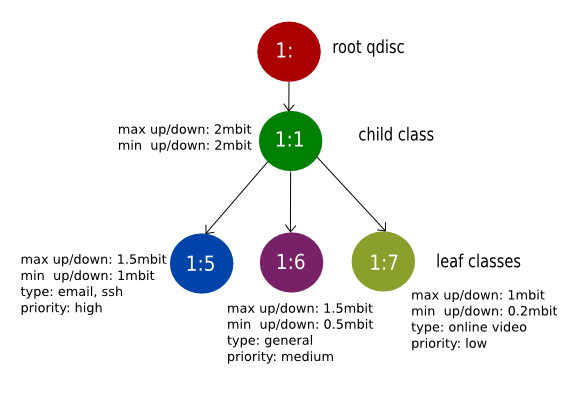
\includegraphics[width=8cm]{archivos/img/teoria/tc_qdisc_example_implementation.png}
    \caption{Sistema de QoS implementado con distintas clases \cite{qdiscs}}
    \label{fig:linuxNet_tc}
\end{figure}

\subsubsection{Filters}

Un filtro es usado para determinar con qué clase debe ser encolado el paquete. Para ello, el paquete siempre debe ser clasificado con una clase determinada. Varios tipos de filtros se pueden utilizar para clasificar los paquetes, pero en este caso será de interés el tipo de filtro \gls{bpf}\footnote{\url{https://man7.org/linux/man-pages/man8/tc-bpf.8.html}}, los cuales permiten anclar un \textit{bytecode} \gls{bpf}. Estos filtros se utilizarán para cargar programas \gls{bpf} que trabajarán en conjunto con \gls{xdp} con la finalidad de lograr el Broadcast. Esto es así, ya que en el \gls{tc} ya se hace uso de la estructura \texttt{sk\_buff} (Ir a \ref{linuxNetworking_skbuff}), por lo que ciertos \textit{helpers} \gls{bpf} para clonar paquetes podrán ser utilizados por \textit{bytecode} anclado en el filtro.


%%%%%%%%%%%%%%%%%%%%%%%%%%%%%%%%%%%%%%%%%%%%%%%%%%%%%%%%%%%%%%%%%%%%%%%%%%%%%%%%%%%%%%%%%%

\subsection{Namespaces}
\label{namespaces}
Una \textit{Namespace} se utiliza para aislar un recurso del sistema en una abstracción que hace  creer a los procesos dentro de dicha \textit{Namespace} que tienen su propia instancia del recurso en cuestión aislada del sistema real.  Los cambios realizados sobre recursos aislados del sistema, son solo visibles para procesos que son pertenecientes a la \textit{Namespace}, pero son invisibles para otros procesos pertenecientes al sistema o a otra \textit{Namespace}.\\
\par
Hay muchos tipos de \textit{Namespaces}, en la tabla \ref{tab:linux_ns} se pueden apreciar todos los tipos que existen a día de hoy. El uso de todos estos tipos de \textit{Namespaces} puede ser muy variado, pero el más importante de todos ellos son los contenedores. Los contenedores son elementos para correr aplicaciones, o herraminetas en un entorno aislado del sistema. A día de hoy, los contenedores más utilizados son los de Docker\footnote{\url{https://www.docker.com/}}, pero, ¿Realmente que hace Docker, qué es Docker?\\
\par

Docker se vale de las bondades del Kernel de Linux para aislar recursos y con esto conformar contenedores. Éste hará uso de las APIs suministradas por el Kernel para crear y destruir a conveniencia las distintas \textit{Namespaces}. Por lo que, Docker en verdad simplemente es un envoltorio de las llamadas al sistema para gestionar \textit{Namespaces}. Docker además, provee de distintos aspectos al usuario como \textit{copy-on-write}, o una configuración en modo \textit{bridge} hacia el exterior, pero en el fondo es
un mero \textit{wrapper} para la gestión de las \textit{Namespaces} con la finalidad de implementar contenedores.

% \begin{table}[ht]
%     \centering
%     \resizebox{\textwidth}{!}{%
%         \begin{tabular}{|l|l|}
%             \hline
%             \rowcolor[HTML]{EFEFEF}
%             \multicolumn{1}{|c|}{\cellcolor[HTML]{EFEFEF}{\color[HTML]{24292E} \textbf{Tipo de Namespace}}} & \multicolumn{1}{c|}{\cellcolor[HTML]{EFEFEF}{\color[HTML]{24292E} \textbf{Descripción}}}                                                                                                                                                     \\ \hline
%             \textbf{Cgroup}                                                                                 & \begin{tabular}[c]{@{}l@{}}Namespace utilizada generalmente para establecer unos limites de recursos,  por ejemplo, \\ CPU, memoria, lecturas y escrituras a disco, de todos los procesos que corran dentro de dicha Namespace.\end{tabular} \\ \hline
%             Time                                                                                            & Namespace para establecer una hora del sistema diferente a la del sistema.                                                                                                                                                                   \\ \hline
%             \textbf{Network}                                                                                & Namespace utilizada para tener una replica aislada del stack de red del sistema, dentro del propio sistema.                                                                                                                                  \\ \hline
%             \textbf{User}                                                                                   & Namespace utilizada para tener aislados a un grupo de usuarios.                                                                                                                                                                              \\ \hline
%             \textbf{PID}                                                                                    & Namespace utilizada para tener identificadores de proceso independientes de otras namespaces.                                                                                                                                                \\ \hline
%             \textbf{IPC}                                                                                    & Namespace utilizada para aislar los mecanismos de comunicación entre procesos.                                                                                                                                                               \\ \hline
%             \textbf{Uts}                                                                                    & Namespace utilizada para establecer un nombre de Host y nombre de dominio diferentes de los establecidos en el sistema                                                                                                                       \\ \hline
%             \textbf{Mount}                                                                                  & Namespace utilizada para aislar los puntos de montaje en el sistema de archivos.                                                                                                                                                             \\ \hline
%         \end{tabular}%
%     }
%     \caption{Resumen de los tipos de Namespaces en el Kernel de Linux}
%     \label{tab:linux_ns}
% \end{table}


\begin{table}[ht]
    \centering
    \resizebox{\textwidth}{!}{%
        \begin{tabular}{|l|l|}
            \hline
            \rowcolor[HTML]{EFEFEF}
            \multicolumn{1}{|c|}{\cellcolor[HTML]{EFEFEF}{\color[HTML]{24292E} \textbf{Tipo de Namespace}}} & \multicolumn{1}{c|}{\cellcolor[HTML]{EFEFEF}{\color[HTML]{24292E} \textbf{Descripción}}}                                                                                                                                   \\ \hline
            \textbf{Cgroup}                                                                                 & \begin{tabular}[c]{@{}l@{}}Namespace utilizado generalmente para establecer límites de recursos,\\ como CPU, memoria, lecturas y escrituras a disco, para todos los procesos\\ dentro de la misma Namespace. \end{tabular} \\ \hline
            Time                                                                                            & \begin{tabular}[c]{@{}l@{}}Namespace utilizado para establecer una hora del sistema diferente\\ a la del sistema global.\end{tabular}                                                                                      \\ \hline
            \textbf{Network}                                                                                & \begin{tabular}[c]{@{}l@{}}Namespace utilizado para crear una réplica aislada del stack de red \\ del sistema dentro del propio sistema.      \end{tabular}                                                                \\ \hline
            \textbf{User}                                                                                   & Namespace utilizado para aislar un grupo de usuarios.                                                                                                                                                                      \\ \hline
            \textbf{PID}                                                                                    & \begin{tabular}[c]{@{}l@{}}Namespace utilizado para tener identificadores de proceso independientes\\ de otras namespaces. \end{tabular}                                                                                   \\ \hline
            \textbf{IPC}                                                                                    & Namespace utilizado para aislar los mecanismos de comunicación entre procesos.                                                                                                                                             \\ \hline
            \textbf{Uts}                                                                                    & \begin{tabular}[c]{@{}l@{}}Namespace utilizado para establecer un nombre de host y nombre de dominio \\ diferentes de los establecidos en el sistema.      \end{tabular}                                                   \\ \hline
            \textbf{Mount}                                                                                  & Namespace utilizado para aislar los puntos de montaje en el sistema de archivos.                                                                                                                                           \\ \hline
        \end{tabular}%
    }
    \caption{Resumen de los tipos de Namespaces en el Kernel de Linux}
    \label{tab:linux_ns}
\end{table}


\subsubsection{Persistencia de las Namespaces}

Atendiendo a la \textit{man-page} \cite{ns} sobre \textit{Namespaces}, es importante señalar que las \textit{Namespaces} tienen una vida finita. La vida finita de la \textit{Namespace} dependerá de si la \textit{Namespace} en cuestión está referenciada, por lo que éstas vivirán siempre y cuando estén referenciadas, cuando dejen de estarlo serán destruidas.\\
\par
Este concepto de vida finita, será útil entenderlo para tener una mejor comprensión sobre el funcionamiento interno de Mininet ó Mininet-WiFI, los cuales se valen de estos conceptos para ahorrarse operaciones y ganar en rendimiento.  Una Namespace a día de hoy puede ser referenciada de tres maneras distintas:\\

\begin{itemize}
    \item Siempre y cuando haya un proceso corriendo dentro de esta \textit{Namespace}.
    \item Siempre que haya abierto un descriptor de archivo al fichero identificativo de la \textit{Namespace} (\texttt{/proc/{pid}/ns/{tipo\_namespace}}).
    \item Siempre que exista un \textit{bind-mount} del fichero (\texttt{/proc/{pid}/ns/{tipo\_namespace}}) de la \textit{Namespace} en cuestión.
\end{itemize}

Si ninguna de estas condiciones se cumple, la \textit{Namespace} en cuestión es eliminada automáticamente por el Kernel. Si se tratase de una \textit{Network Namespace}, aquellas interfaces que se encuentren en la \textit{Namespace} en desaparición volverán a la \textit{Network Namespace} por defecto \cite{ns}.

\subsubsection{Concepto de las Network Namespaces}

Una vez entendido el concepto de \textit{Namespace} en Linux, se introducen las \textit{Network Namespace}, las cuales serán fundamentales para las plataformas donde se probarán los distintos test. Éstas consisten en una replica lógica de \textit{stack} de red que por defecto tiene Linux, replicando rutas, tablas ARP, Iptables e interfaces de red \cite{netns}. \\
\par
Linux se inicia con un \textit{Network Namespace} por defecto, el espacio \textit{root}, con su tabla de rutas, su tabla ARP,  Iptables e interfaces de red. Pero también es posible crear más \textit{Network Namespace} no predeterminadas,  crear nuevos dispositivos en esos espacios de nombres, o mover un dispositivo existente de un espacio de nombres a otro. \\
\par
Para llevar todas estas tareas a cabo, la herramienta más sencilla será \texttt{iproute2} (Ir a Anexo \ref{iproute2}). Esta herramienta, haciendo uso del módulo \texttt{netns}, se podrá gestionar todo en lo relativo a las \textit{Network Namespace} con nombre. Esta coletilla, ``con nombre", atiende a que todas las \textit{Network Namespace} que se gestionen desde \texttt{iproute2} serán persistentes debido a que se realizará un \textit{bind-mount} con el nombre de la \textit{Namespace}, del fichero identificativo de la \textit{Namespace} en cuestión, bajo el directorio \texttt{/var/run/netns} . A continuación, se listan los comandos más frecuentes a la hora de gestionar \textit{Network Namespaces}, se entiende que se ejecutan con permisos de súper usuario.

\begin{lstlisting}[language= bash, style=Consola, caption={Comandos útiles con iproute2 - Netns},label=code:iproute2_ns_use]
    # Para crear una Network Namespace
    ip netns add {nombre netns}
    
    # Para listar las Network Namespaces "con nombre"
    ip netns list
    
    # Para añadir una interfaz a una Network Namespace
     ip netns set {nombre netns} Veth
    
    # Para ejecutar un comando dentro de una Network Namespace
    ip netns exec {nombre netns} {cmd}
    
    # Para eliminar una Network Namespace
    ip netns del {nombre netns}
    
\end{lstlisting}

\subsubsection{Métodos de comunicación inter-Namespaces: \glsentryshort{veth}}
\label{linuxVeths}
Las \gls{veth}, son interfaces de Ethernet virtuales creadas como un par de interfaces interconectadas entre si. El modelo funcional es sencillo, los paquetes enviados desde una son recibidos por la otra interfaz de forma directa, bastante parecido al funcionamiento de las \textit{pipes}. Una condición interesante de estas interfaces es que su gestión está asociada, es decir, si se levanta una extremo de la \gls{veth}, la otra también lo hará, si por el contrario se deshabilita o se destruye algún extremo de un par de \gls{veth} el otro extremo también se verá afectado \cite{veth}.\\
\par
Es muy común hacer uso de las \gls{veth} para interconectar \textit{Network Namespaces}, ya que, sabiendo que estas van a estar conectadas de forma directa, se puede utilizar este enlace como pasarela entre dos \textit{Network Namespaces}. De esta forma, se estaría interconectando dos \textit{stacks} independientes de red. La creación y destrucción de este tipo de interfaces se puede apreciar en el bloque \ref{code:iproute2_veth_use}, se recuerda que es necesario permisos de súper usuario.\\

\begin{lstlisting}[language= bash, style=Consola, caption={Manejo de Veths},label=code:iproute2_veth_use]
    # Crear un par veth
    ip link add {nombre_veth1} type veth peer name {nombre_veth2}
    
    # Si se elimina un extremo, el otro también lo hará
    ip link delete {nombre_veth}
    
\end{lstlisting}
\vspace{0.5cm}

Por lo tanto, se puede llegar al siguiente diagrama básico del funcionamiento de un par de \gls{veth}, las cuales estarán asignadas a una \textit{Network Namespace} distinta.  Como se puede apreciar en la figura \ref{fig:linuxNet_veth}, ambas interfaces están conectadas entre si directamente de forma interna en el propio Kernel. En el caso de que se generen paquetes desde una \textit{Network Namespace} hacia la otra, estos paquetes llegarán desde un extremo de la \gls{veth} directamente al otro extremo de la \gls{veth} a través del Kernel, y en este caso, la \textit{Network Namespace} por defecto no percibirá dicho trafico.\\
\par
Esta condición será de gran utilidad para recrear enlaces entre nodos independientes de red, los nodos se replicarán con \textit{Network Namespaces} y los enlaces con \gls{veth}s. Estos mecanismos serán utilizados por herramientas de emulación de redes como Mininet o Mininet-WiFI, más adelante se destallará.

\begin{figure}[ht]
    \centering
    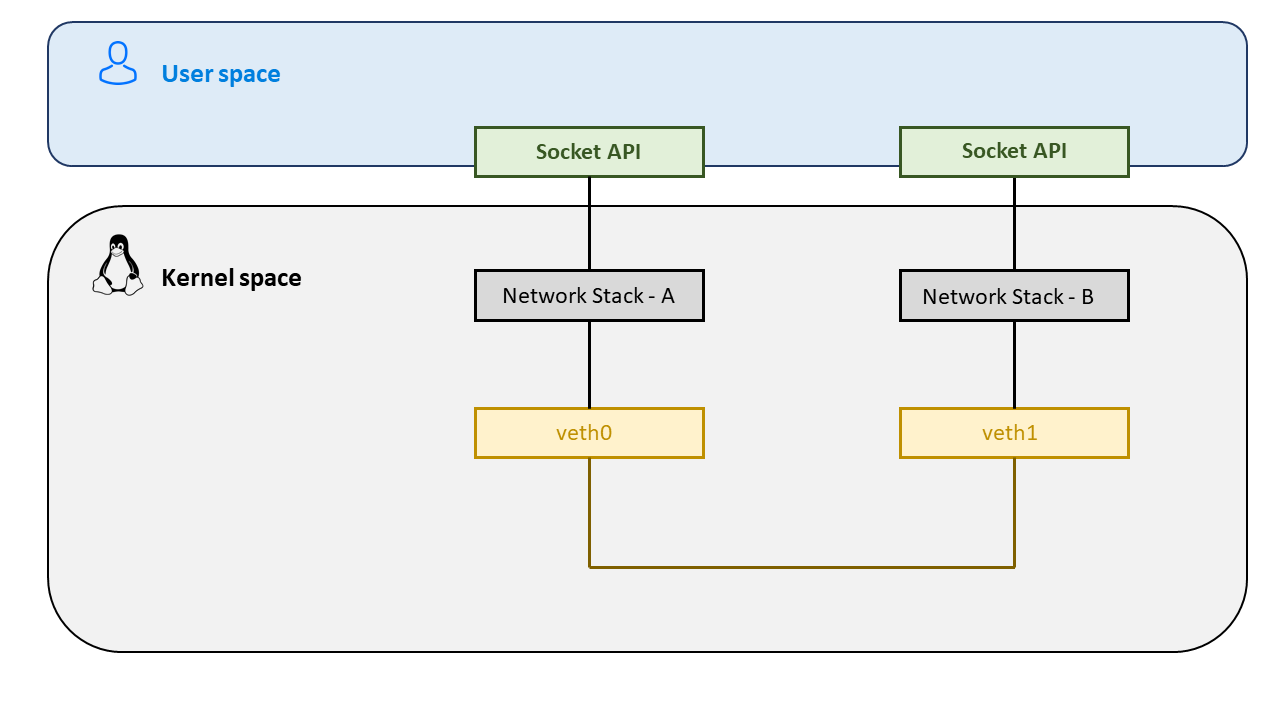
\includegraphics[width=15.5cm]{archivos/img/teoria/user_kernel.png}
    \caption{Enlace entre interfaces Veth separadas en dos Network Namespaces}
    \label{fig:linuxNet_veth}
\end{figure}

%%%%%%%%%%%%%%%%%%%%%%%%%%%%%%%%%%%%%%%%%%%%%%%%%%%%%%%%%%%%%%%%%%%%%%%%%%%%%%%%%%%%%%%%%%%%%%%%%%%%%
% Mininet & Mininet-Wifi
\section{Mininet y Mininet-WiFi}
\label{sec:mininet}

En esta sección se abordará el marco teórico relacionado con las principales herramientas de emulación utilizadas en este proyecto. Se prestará especial atención a Mininet, que es la herramienta principal y la base sobre la cual han surgido otras herramientas de emulación, como Mininet-WiFi y Mininet-IoT.\\

\subsection{Mininet}

Mininet es una herramienta utilizada para emular redes, principalmente del tipo SDN (Software-Defined Networking). Permite emular hosts, routers, switches y enlaces en una sola máquina a un coste reducido, siempre y cuando se cuente con el Kernel de Linux en dicha máquina. Para lograr esto, Mininet utiliza una forma de virtualización "ligera" que aprovecha las capacidades del Kernel de Linux para virtualizar recursos, como las \textit{Namespaces} (consultar \ref{namespaces}) \cite{lantz2010network}.\\
\\
La cantidad de recursos virtualizados dependerá de las características de cada nodo, y esto también afectará el rendimiento de la emulación. Por ejemplo, los nodos tipo \texttt{Host} en Mininet requieren el uso de una \textit{Network Namespace}, lo que les proporciona su propio \textit{stack} de red y los hace completamente independientes\footnote{En lo que respecta a Networking} del sistema y otros nodos en la red emulada. Sin embargo, por defecto, todos los nodos \texttt{Host} comparten el sistema de archivos, la numeración de procesos (PIDs), los usuarios, etc. En términos técnicos, no están completamente aislados como un host real. Esto se debe a que Mininet virtualiza solo los recursos necesarios para llevar a cabo la emulación, lo que mejora el rendimiento y permite que máquinas con recursos limitados puedan realizar la emulación \cite{lantz2010network}.\\
\\
En cuanto a la creación de topologías en Mininet, existen dos enfoques. El primero es utilizar la API escrita en Python para interactuar con las clases de Mininet. Con esta API, se puede construir la topología importando los módulos y clases necesarios para definirla en un script de Python. El segundo enfoque es utilizar la herramienta llamada \textbf{MiniEdit}, que proporciona una interfaz gráfica (GUI) donde los usuarios pueden crear la topología arrastrando y soltando nodos de red. Desde la misma GUI, se puede exportar la topología generada a un archivo (\texttt{*.mn}) para recuperarla más tarde o a un script en Python (\texttt{*.py}) para cargarla en el intérprete de Python cuando sea necesario. Esta herramienta es especialmente útil para aquellos que no tienen conocimientos de programación en Python pero desean utilizar el emulador, lo que representa una ventaja significativa \cite{lantz2010network}.\\

Por lo tanto, se puede concluir que los aspectos más fuertes de Mininet son los siguientes puntos:

\begin{itemize}
    \item Mininet es rápido gracias a su diseño basado en \textit{Namespaces}, lo que permite una gestión eficiente de los recursos. En la sección \ref{namespaces}, se explica cómo se lleva a cabo esta gestión.
    \item Mininet no consume recursos en exceso, ya que virtualiza únicamente los componentes necesarios para la emulación. Además, se pueden establecer límites máximos de recursos para la emulación en caso de ser necesario.
    \item Mininet brinda libertad al usuario para crear topologías y escenarios personalizados utilizando la API en Python de Mininet. Estos escenarios pueden ser fácilmente transferidos a otra máquina, ya que solo se requiere compartir el script que describe la topología. Es importante tener en cuenta que los resultados de las pruebas pueden variar entre diferentes máquinas, ya que Mininet emula la red en lugar de simularla. Por lo tanto, los resultados dependerán de las condiciones de la máquina donde se ejecuten las pruebas.
\end{itemize}

Aunque Mininet ofrece muchas ventajas, también tiene una limitación importante que debe tenerse en cuenta. Como se mencionó anteriormente, Mininet utiliza una forma de virtualización ``ligera" basada en las \textit{Namespaces} del Kernel de Linux. Si bien esta decisión de diseño proporciona beneficios significativos en términos de rendimiento al aprovechar el propio sistema operativo para virtualizar recursos, surge un problema cuando se intenta exportar el emulador a otra plataforma con un sistema operativo diferente. Es posible que este sistema operativo no admita un equivalente funcional a las \textit{Namespaces} de Linux o, incluso si lo hace, su API para utilizarlas puede ser completamente diferente. Esto puede dificultar o incluso impedir la ejecución de Mininet en plataformas que no porten el kernel de Linux.


\subsection{Funcionamiento de Mininet}

Anteriormente se mencionó que Mininet utiliza \textit{Network Namespaces} como método para virtualizar \textit{stacks} de red independientes y así emular redes con un costo mínimo. En la figura \ref{fig:mininet_arch}, se muestra la arquitectura interna de Mininet para una topología compuesta por dos nodos \texttt{Host} y un software switch conectado por TCP a un controlador remoto.\\
\\
Como se puede observar, cada nodo \texttt{Host} está aislado en su propia \textit{Namespace} de red, mientras que el switch se ejecuta en la \textit{Namespace} por defecto (root). La comunicación entre los nodos de esta topología se realiza mediante \gls{veth}s (consultar \ref{linuxVeths}), las cuales permiten emular los enlaces entre los diferentes nodos de la red.\\

%fig
\begin{figure}[ht]
    \centering
    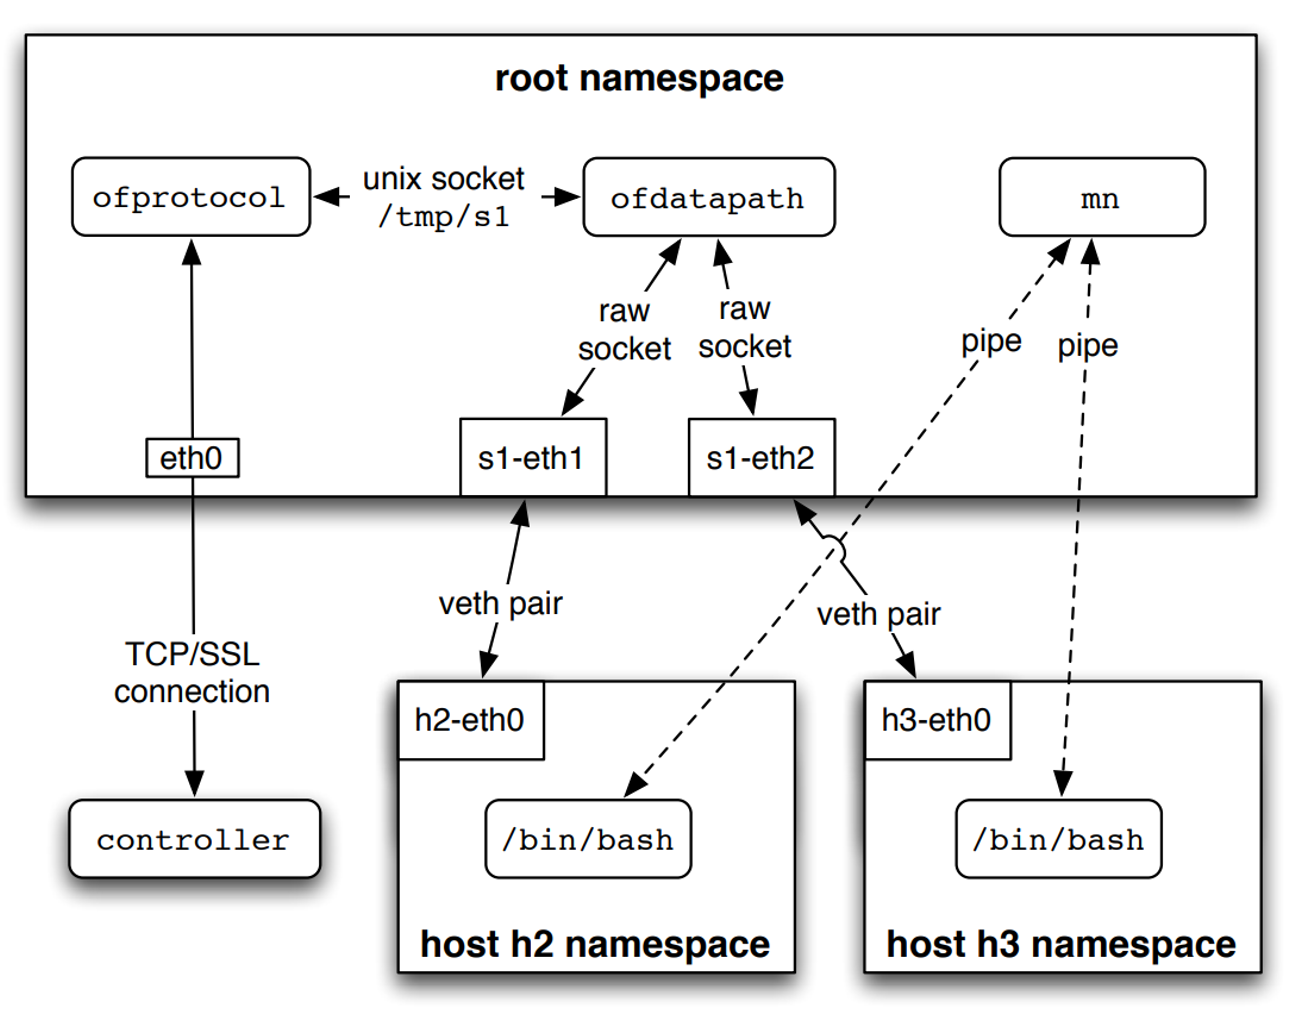
\includegraphics[width=\textwidth]{archivos/img/teoria/mn_arch.png}
    \caption{Arquitectura de Mininet \cite{heller2013reproducible}}
    \label{fig:mininet_arch}
\end{figure}

Una vez presentada toda la teoría sobre Mininet, puede surgir la pregunta de cómo se puede comprobar si realmente utiliza \textit{Network Namespaces}. Para hacerlo, lo primero que se debe hacer es crear el escenario para que Mininet pueda crear las \textit{Network Namespaces} necesarias. En este caso, se utilizará la topología mostrada en la figura \ref{fig:mininet_arch}. Para crear esta topología, solo se necesita tener Mininet instalado y seguir los pasos que se indican en el bloque \ref{code:scenarioMininet}. Una vez levantado el escenario, se debería obtener el output indicado en la figura \ref{fig:mininet_01}.


\begin{lstlisting}[language= bash, style=Consola, caption={Ejecución de Mininet con la topología por defecto},label=code:scenarioMininet]
    # Lanzamos Mininet con la topo por defecto :)
    sudo mn
    
\end{lstlisting}
\vspace{0.5cm}

\begin{figure}[ht]
    \centering
    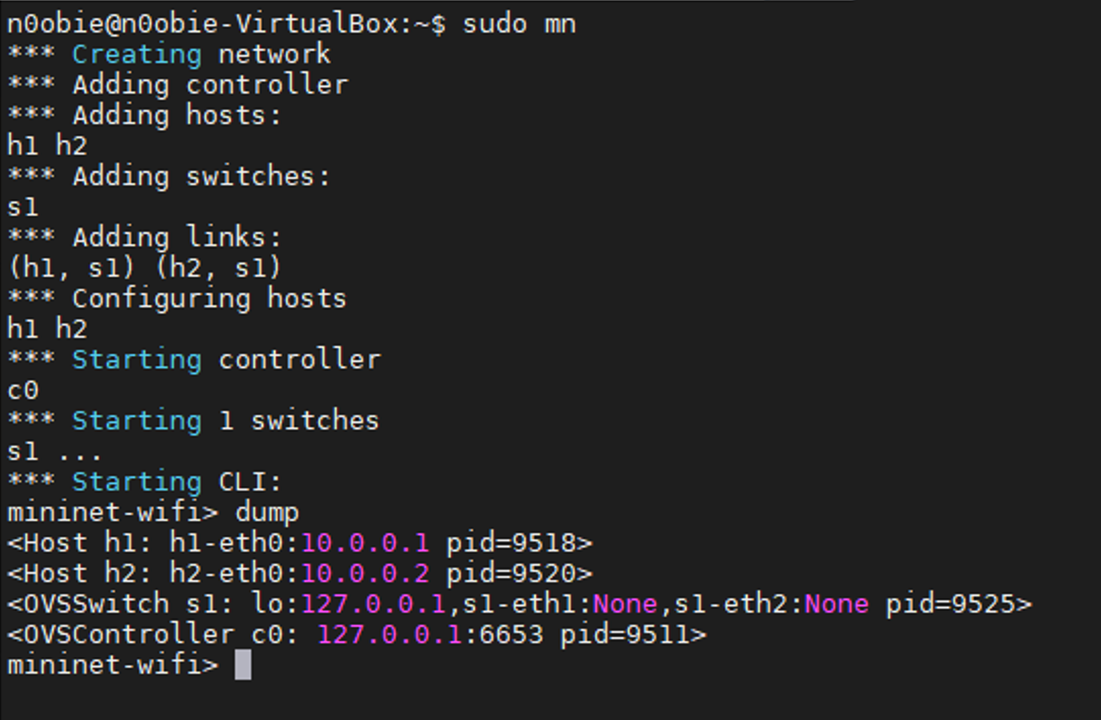
\includegraphics[width=0.7\textwidth]{archivos/img/teoria/mn_01.png}
    \caption{Salida por pantalla de la ejecución de la topología por defecto}
    \label{fig:mininet_01}
\end{figure}

Ahora que hemos creado el escenario, podemos verificar si hay \textit{Network Namespaces} en el sistema utilizando el conjunto de herramientas iproute2 (consultar \ref{iproute2}). El comando más utilizado para listar las \textit{Network Namespaces} utilizando el módulo \textbf{netns} se muestra en el bloque \ref{code:MininetNs}.


\begin{lstlisting}[language= bash, style=Consola, caption={Listar Named Network Namespaces},label=code:MininetNs]
    # Listamos las network namespaces con Nombre! ojito :)
    sudo ip netns list
\end{lstlisting}
\vspace{0.5cm}

\begin{figure}[ht]
    \centering
    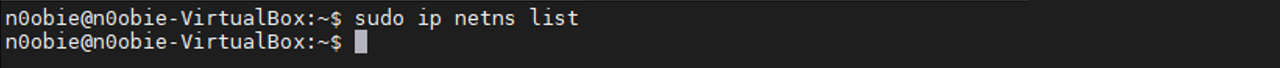
\includegraphics[width=\textwidth]{archivos/img/teoria/mn_02.png}
    \caption{Listado de Named Network Namespaces existentes en el sistema}
    \label{fig:mininet_02}
\end{figure}


Al observar la figura \ref{fig:mininet_02}, no parece haber ninguna \textit{Network Namespace} en el sistema. Entonces, ¿dónde está el problema? La razón por la que el comando \texttt{ip netns list} no muestra información es que Mininet no está creando el enlace simbólico (\textit{softlink}) necesario para que la herramienta pueda listar las \textit{Network Namespaces}. Según la documentación del comando, este lee desde la ruta \texttt{/var/run/netns/}, donde se encuentran todas las \textit{Network Namespaces} con nombre. Estas Netns son aquellas en las que se ha realizado un \textit{bindmount} con su nombre en ese directorio para que persistan incluso si no hay ningún proceso en ejecución en ellas.Como se mencionó anteriormente, las \textit{Namespaces} tienen una vida finita y solo existen mientras estén referenciadas (consulte la tabla \ref{tab:linux_ns}). Por lo tanto, si no se cumple ninguna condición de referencia, la \textit{Namespace} en cuestión se elimina.\\
\\
Mininet se encarga de recrear la red emulada y, cuando el usuario finaliza la emulación, la red emulada debe desaparecer. Este proceso debe ser lo más rápido y eficiente posible para brindar una mejor experiencia al usuario. La naturaleza del diseño de Mininet sugiere que la creación y destrucción de las \textit{Network Namespaces} están asociadas con la primera condición de referencia de una \textit{Namespace}.\\
\\
En otras palabras, no tendría sentido realizar enlaces o enlaces simbólicos que luego se deban eliminar, ya que esto implicaría una carga de trabajo significativa para emulaciones de redes grandes y aumentaría el tiempo necesario para limpiar el sistema una vez finalizada la emulación. Además, hay que tener en cuenta que existe una condición que se adapta bien a las necesidades de Mininet: solo se requiere un proceso en ejecución por cada \textit{Network Namespace}, y al realizar la limpieza, solo se deben finalizar los procesos que mantienen las \textit{Network Namespaces}. Cuando no haya más procesos en ejecución en una \textit{Namespace}, el kernel se encargará de eliminarla.\\
\\
De acuerdo con el razonamiento expuesto, se deberían ver varios procesos que se crean al iniciar el escenario en Mininet. Cada uno de estos procesos deberá tener un archivo de \textit{Network Namespace} (\texttt{/proc/{pid}/ns/net}) con un número de nodo único (\textit{inode}) para los procesos que se ejecutan en diferentes \textit{Network Namespaces}.\\

\begin{figure}[ht]
    \centering
    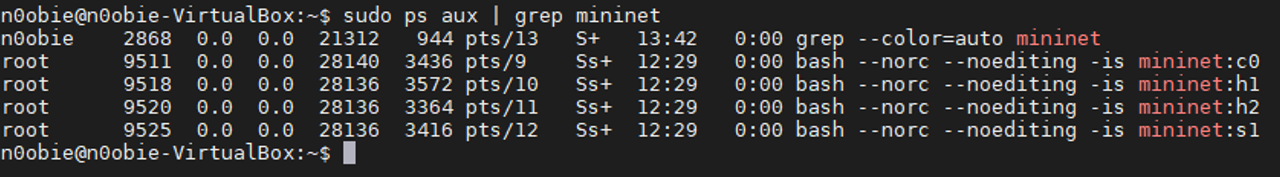
\includegraphics[width=\textwidth]{archivos/img/teoria/mn_03.png}
    \caption{Listado de procesos con referencias a Mininet}
    \label{fig:mininet_03}
\end{figure}

Si examinamos el archivo \texttt{/proc/{pid}/ns/net} para cada proceso mencionado en la figura \ref{fig:mininet_03}, podremos determinar cuáles de ellos se encuentran en una \textit{Network Namespace} distinta, según el valor del \textit{inode}. Por ejemplo, verifiquemos los procesos asociados a los \texttt{Host1} y \texttt{Host2}.\\


\begin{figure}[ht]
    \centering
    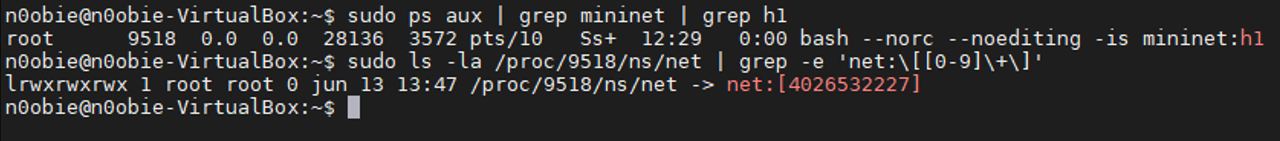
\includegraphics[width=\textwidth]{archivos/img/teoria/mn_04.png}
    \caption{Información de contexto sobre el proceso del Host1}
    \label{fig:mininet_04}
\end{figure}

\newpage

\begin{figure}[ht]
    \centering
    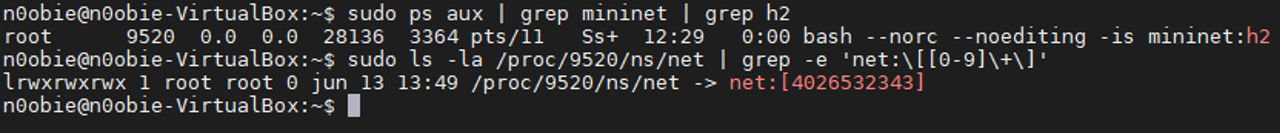
\includegraphics[width=\textwidth]{archivos/img/teoria/mn_05.png}
    \caption{Información de contexto sobre el proceso del Host2}
    \label{fig:mininet_05}
\end{figure}

Como se puede observar, hay diferentes \textit{inodes}, archivos distintos y \textit{Network namespaces} diferentes. Esta prueba demuestra cómo Mininet utiliza procesos de bash para mantener las \textit{Network Namespaces} de los nodos que lo requieren.


\subsection{Mininet-WiFi}

Mininet-WiFi \cite{7367387} es un emulador de redes inalámbricas diseñado principalmente para trabajar bajo el estándar \texttt{ieee80211}. Esta herramienta nació de Mininet, es decir, es un \textit{fork} de la misma. Por ello, comparten todas las bases sobre virtualización ``ligera" haciendo uso de \textit{Namespaces} y \gls{veth}s, por tanto, todos los scripts de Mininet son compatibles en Mininet-WiFi. \\
\par
Esto es así ya que toda la funcionalidad wireless es un añadido sobre la base que desarrollaron para Mininet. Los desarrolladores de Mininet-WiFi se valieron del subsistema wireless del Kernel de Linux y del módulo mac80211\_hwsim, para conseguir emular las interfaces y el supuesto medio inalámbrico. Para más información sobre esta herramienta se recomienda ir al \textbf{punto} \ref{mn-wifi_bmv2_integration}, donde se hace un análisis profundo sobre las jerarquías de clases añadidas en Mininet-WiFi, como opera internamente y como se comunica con el módulo en el kernel para generar los escenarios inalámbricos.



\subsection{Mininet-IoT}
\label{mininetIoT}

La herramienta Mininet-IoT \cite{mininetIOT} es un emulador de redes de baja capacidad diseñado para trabajar en conjunto bajo el estándar \texttt{ieee802154} y la capa de adaptación 6LoWPAN. Esta herramienta nació de Mininet-WiFi, que a su vez nació de Mininet, por lo que en la práctica, Mininet-IoT comparte todas las técnicas de virtualización ``ligera" de Mininet. Al heredar de Mininet-WiFi y Mininet, todos los scripts para desplegar topologías alámbricas y WiFi son compatibles en Mininet-IoT.  \\
\par

La gran diferencia entre Mininet-IoT y Mininet-WiFi, radica en el módulo que emplean para conseguir emular las interfaces y el supuesto medio inalámbrico. Mininet-WiFi hace uso del módulo mac80211\_hwsim, mientras que Mininet-IoT hace uso del módulo del Kernel mac802154\_hwsim (es necesario tener una versión del Kernel superior a la \texttt{4.18.x} para obtener dicho modulo). Toda la gestión de nodos, interfaces y enlaces es exactamente la misma a la de Mininet-WiFi. Por ello, Ramon Fontes (principal desarrollador de la herramienta), creó una clase agnóstica para gestionar módulos del Kernel en Mininet-WiFi, y migró todo el proyecto de Mininet-IoT a Mininet-WiFi. De esta forma, el mantenimiento del \textit{core} que compartían ambas herramientas se hacía únicamente en un proyecto, y daba la posibilidad al usuario de Mininet-WiFi de establecer enlaces de baja capacidad en sus topologías inalámbricas.

%%%%%%%%%%%%%%%%%%%%%%%%%%%%%%%%%%%%%%%%%%%%%%%%%%%%%%%%%%%%%%%%%%%%%%%%%%%%%%%%%%%%%%%%%%%%%%%%%%%%%
% Controladores SDN (Ryu & Onos)
\section{Controladores \glsentryshort{sdn}}
\label{sec:sdnControllers}

Los controladores \gls{sdn}, también conocidos como sistemas operativos de red, son una pieza clave en los entornos  \gls{sdn} dado que tienen una vista global de toda la red que gestionan, que flujos atraviesan la red, estadísticas, usuarios finales, modelos y características de dichos equipos. Este controlador tiene la funcionalidad de interconectar los recursos disponibles en la red que gestiona, a aplicaciones o servicios que corran encima de él \cite{nadeau2013sdn}. De esta forma, cada vez que se quiera añadir una nueva funcionalidad, solo se tendrá que programar un nuevo servicio que corra encima del controlador que gestiona la red, y este a su vez se encargará de traducir las demandas del servicio a políticas de red a cada dispositivo impactado. En este matiz se puede llegar apreciar el sentido de nombre del paradigma \gls{sdn}, ya que estamos definiendo por software el comportamiento intrínseco de la red.\\
\\
% fig
\begin{figure}[ht]
    \centering
    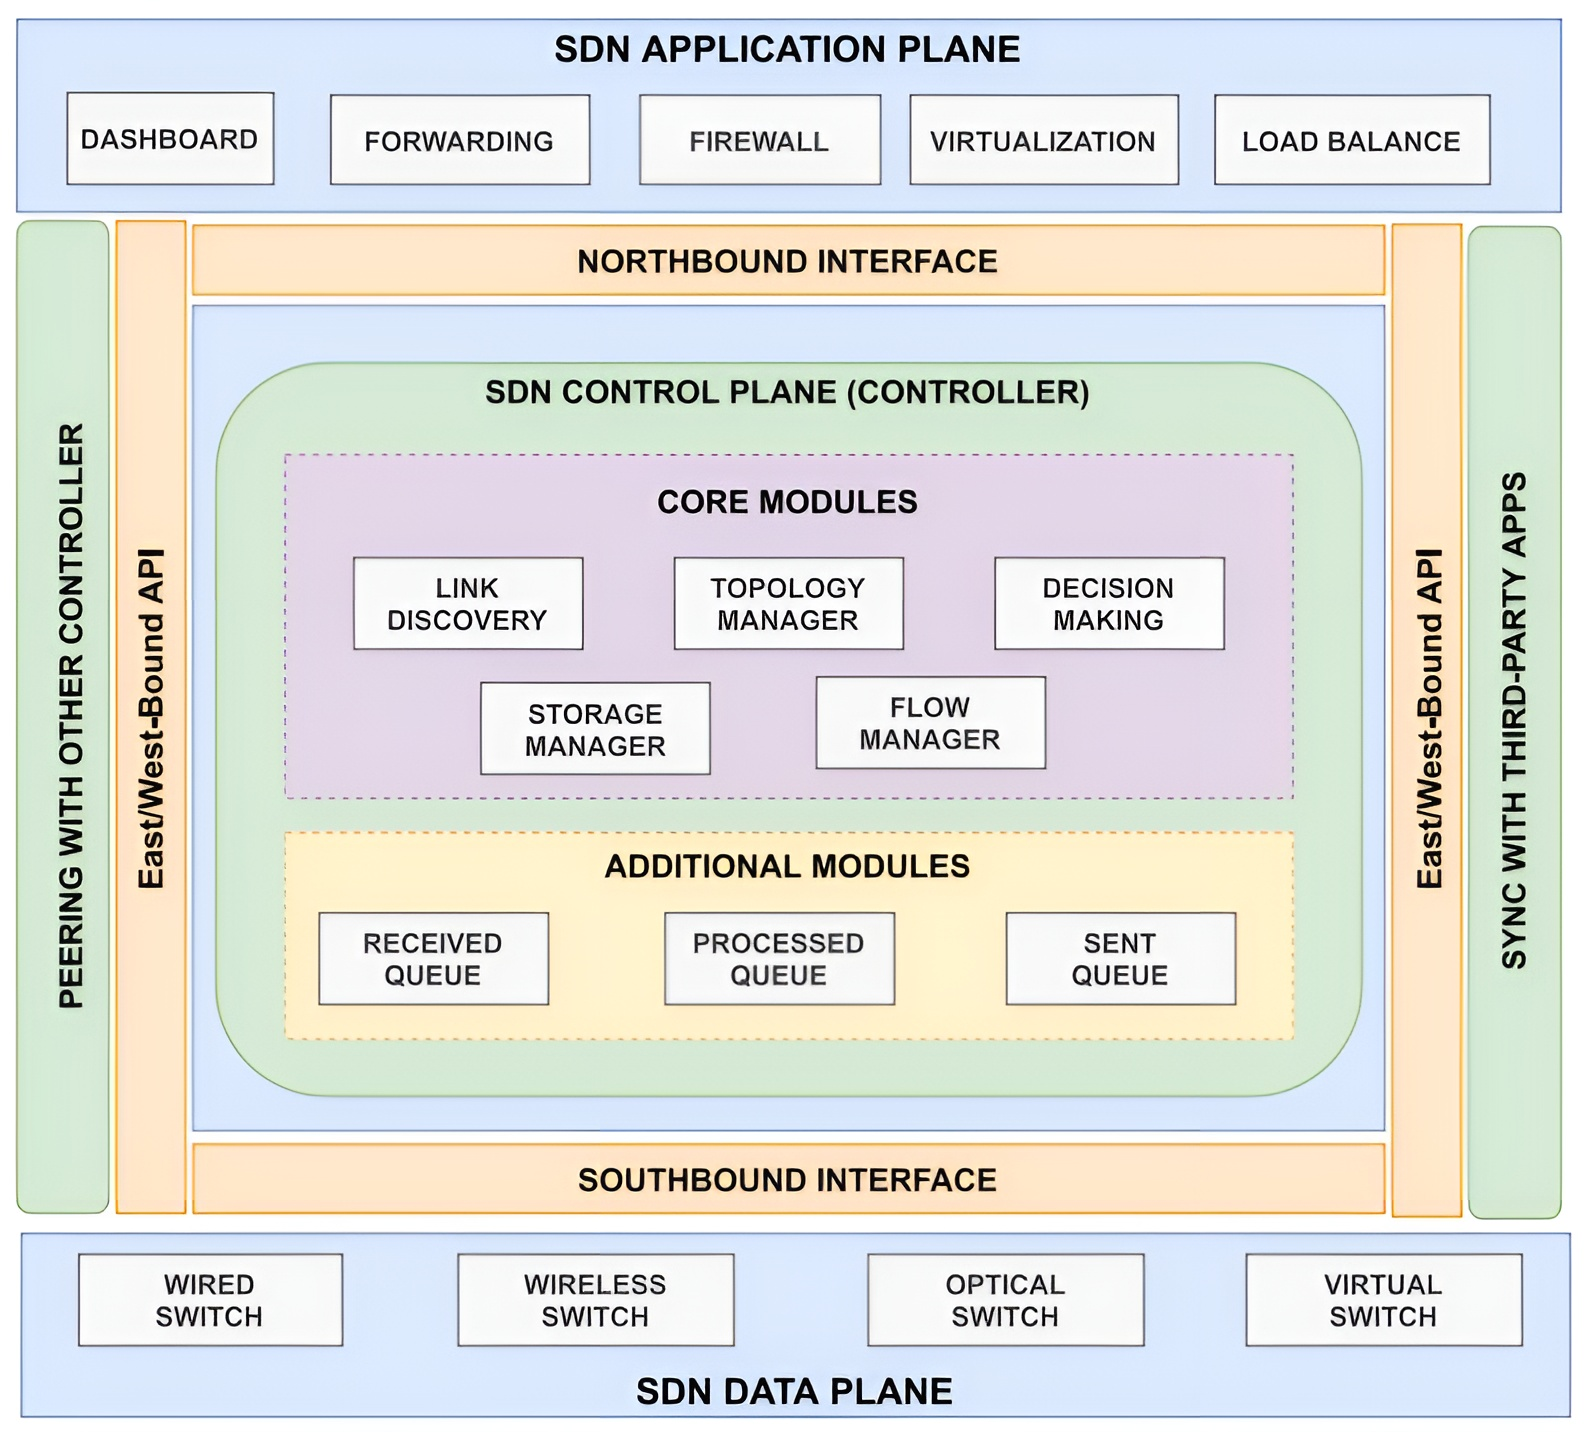
\includegraphics[width=\textwidth]{archivos/img/teoria/sdn_controllers.jpg}
    \caption{Arquitectura generica de controlador \glsentryshort{sdn} \cite{zhu2020sdn}}
    \label{fig:sdn_controllers}
\end{figure}

En la literatura hay muchas propuestas de arquitecturas para los controladores, pero en vez de ir una por una viendo las diferencias vamos a presentar la arquitectura genérica que se puede encontrar en la gran mayoría de controladores \gls{sdn}. Si nos fijamos en la Figura \ref{fig:sdn_controllers}, podemos ver dos partes claramente diferenciadas, el núcleo del controlador y las interfaces del mismo \cite{zhu2020sdn}. Empezando por el \textit{core}, se puede resumir que las funciones básicas del controlador están relacionadas principalmente con el descubrimiento de la topología y la gestión de los flujos de tráfico. El módulo de descubrimiento de la topología suele trabajar con el protocolo \gls{lldp}. La implementación puede variar entre controladores y aplicaciones de descubrimiento topológico, pero en términos generales, se transmite regularmente consultas utilizando mensajes \texttt{packet\_out}, los cuales viajaran por la topología física y volverán al controlador en forma de mensajes \texttt{packet\_in}, que permiten al controlador construir la topología de la red.\\
\\
Una vez que se conoce la topología de red, el controlador puede empezar a poner en marcha distintos módulos de toma de decisiones para encontrar los caminos óptimos entre los nodos de la red. Con todos los caminos ya construidos, entran en juego otros módulos del controlador como son \gls{qos} y de seguridad, los cuales pueden optar por instalar una ruta sub-óptima para satisfacer los criterios de \gls{qos} o de seguridad. De forma adicional, el controlador puede tener un recopilador de estadísticas y un gestor de colas para recopilar información sobre el rendimiento de las diferentes colas de paquetes entrantes y salientes de los dispositivos de red que gestiona, y con ellos realimentar a los módulos de \gls{qos}. Por último, tenemos uno de los módulos más importantes del controlador, el gestor de flujos. El gestor de flujos, puede variar su implementación en función de los protocolos que se utilicen en la \gls{sbi}, pero su misión es la misma, instalar reglas en los dispositivos de red que gestiona las directrices necesarias para gestionar los paquetes de un determinado flujo de una determinada manera. \\
\\
Siguiendo con otra parte fundamental del controlador \gls{sdn} genérico, son las interfaces. El controlador está rodeado de interfaces para interactuar con otras capas, superior e inferior, y otros controladores, este y oeste (E-WBIs). Empezando por la interfaz \gls{sbi}, la cual es la encargada de interconectar dispositivos \gls{sdn} con el controlador, define un conjunto de reglas, que variarán en función del protocolo que se utilice, las cuales permiten definir el procesamiento y las políticas de reenvío de los dispositivos \gls{sdn}. El protocolo OpenFlow es unas de las \gls{sbi} más utilizadas, y es un estándar de facto para la industria, con el cual podemos es definir flujos y clasificar el tráfico de red basándose en un conjunto de reglas predefinidas. Pero también se pueden encontrar otras \gls{sbi}, como por ejemplo, P4Runtime de facto el futuro para las \gls{sbi}s, o podemos encontrar algunas más \textit{legacy}, como por ejemplo, Netconf o incluso \gls{snmp}.\\
\\
Si nos vamos de la API sur, al norte, encontraremos la conocida como \gls{nbi}, la cual interconecta el controlador \gls{sdn} con las aplicaciones de los desarrolladores o los servicios que definan el comportamiento intrínseco de la red. Los controladores admiten varias interfaces de programación de aplicaciones (API) northbound, pero la mayoría de ellas se basan en la API REST. Generalmente se quiere que la interfaz \gls{nbi} sea una interfaz genérica para que limite a los desarrolladores. Para la comunicación entre controladores, se utilizan las interfaces conocidas como de este y oeste (E/WBI), las cuales no tienen una interfaz de comunicación estándar, por lo que, en función del controlador se tendrá una implementación u otra.\\
\\
A continuación, se presentan dos de los controladores \gls{sdn} más populares: Ryu y \gls{onos}, indicando algunas de sus virtudes y funcionamiento en particular, si bien existen otros como Floodlight, OpenDaylight, etc.

\subsection{Ryu}
\label{subsec:ryu}

Ryu\footnote{Del Japonés, significa ``flujo" y también ``dragón", ambos símbolos Kanji se leen igual como RYU, de ahí que el logo sea un dragón.} es un controlador de red de código abierto diseñado específicamente para redes \gls{sdn}. Se desarrolló en Python por el equipo de NTT (\textit{Nippon Telegraph and Telephone}) y proporciona una plataforma flexible, sencilla y extensible para desarrollar aplicaciones de red basadas en SDN. Como se comentó anteriormente, la funcionalidad primordial que lleva a cabo es la de ser un intermediario entre los elementos de red, como por ejemplo switches SDN o nodos virtuales, y las aplicaciones o servicios que controlan la red a través de la \gls{nbi} \cite{tomonori2013introduction}. De esta forma, a través de la \gls{nbi}, permite a los desarrolladores programar el comportamiento de la red de manera dinámica y centralizada, facilitando la implementación de políticas de red, la configuración de routing y la gestión de tráfico.\\
\\
Ryu es altamente modular y proporciona una API bien definida que permite a los desarrolladores construir aplicaciones de red personalizadas hasta el más mínimo nivel. También es compatible con varios protocolos de comunicación utilizados en SDN, como OpenFlow (versiones \texttt{1.0, 1.2, 1.3, 1.4, 1.5}), NETCONF y OF-config \cite{tomonori2013introduction}.  Las aplicaciones Ryu son entidades que implementan varias funcionalidades dentro de Ryu y se comunican entre sí a través de eventos. Los eventos sirven como mensajes intercambiados entre las aplicaciones Ryu. Estas aplicaciones se envían eventos asíncronos entre sí, creando un flujo de comunicación. Además de las aplicaciones Ryu, existen ciertas fuentes de eventos internas al propio Ryu. Un ejemplo de estas fuentes de eventos es el controlador OpenFlow. Cada aplicación Ryu posee una cola de recepción específicamente diseñada para eventos. La cola funciona según el principio \gls{fifo}, lo que garantiza que se mantenga el orden de los eventos. Para procesar estos eventos, cada aplicación Ryu tiene un único hilo dedicado responsable de la gestión de eventos. Este subproceso vacía continuamente la cola de recepción retirando los eventos de la cola e invocando al manejador de eventos apropiado en función del tipo de evento \cite{ryu1}.

% fig
\begin{figure}[ht]
    \centering
    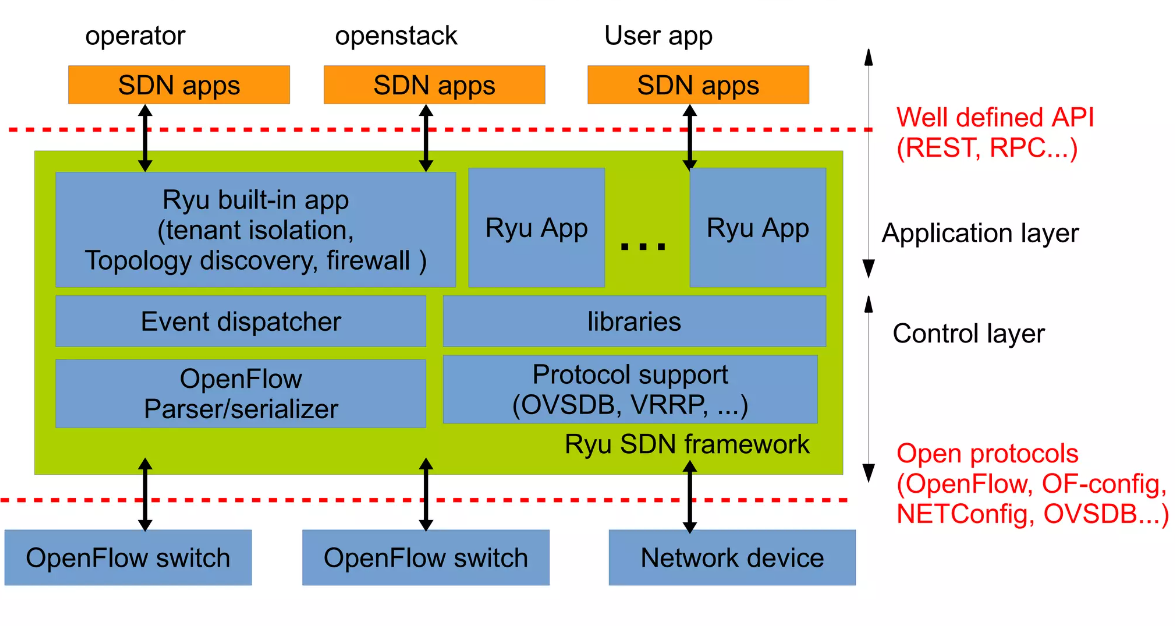
\includegraphics[width=0.85\textwidth]{archivos/img/teoria/ryu.png}
    \caption{Arquitectura del controlador \glsentryshort{sdn} RYU \cite{ryu2}}
    \label{fig:ryu}
\end{figure}

En la Figura \ref*{fig:ryu}, se puede apreciar como la arquitectura del controlador está divida en dos grandes bloques de acuerdo se han estudiado los controladores \gls{sdn}, la parte de \textit{core} y la parte de interfaces. En la parte del núcleo se puede apreciar como se a programado todas las librerías y el manejador de eventos que se mencionaba anteriormente. Por otro lado también se puede apreciar las capas de adaptación a la \gls{sbi} y a la \gls{nbi}, la primera de ellas se adapta a través de una API REST a servicios de aplicaciones externas, mientas que la interfaz \gls{sbi} implementa todos los protocolos de control \gls{sdn}. Algunas de las características y funcionalidades de Ryu incluyen:

\begin{itemize}
    \item Compatibilidad con múltiples protocolos SDN de la interfaz \gls{sbi}.
    \item Capacidad para implementar políticas de red y reglas de enrutamiento de forma sencilla.
    \item Soporte para la recopilación y el análisis de datos de red en tiempo real.
    \item Funcionalidad de control de \gls{qos}.
    \item La más importante de todas, fácil desarrollo y portabilidad sencilla al estar escrita en Python. Esta última se puede ver también como una desventaja, dado el pobre rendimiento de un lenguaje interpretado.
\end{itemize}

Ryu es utilizado en una amplia gama de entornos, desde laboratorios de investigación hasta en las clases de forma educativa. Esta herramienta suele ser el punto de estrada para muchas personas que se inician en el \gls{sdn}, sin embargo, al tener un pobre rendimiento, y la falta de abstracción con los protocolos que se usen en la interfaz \textit{southbound}, hace que en entornos comerciales no se suela ver con tanta frecuencia \cite{tomonori2013introduction}.

\subsection{ONOS}
\label{subsec:ONOS}

\gls{onos} es un controlador de red de código abierto diseñado específicamente para redes \gls{sdn}. Como su nombre indica, \gls{onos} es un sistema operativo para redes que proporciona funcionalidades avanzadas de control y gestión de redes. \gls{onos} está diseñado para ser escalable, confiable y de alto rendimiento, lo que lo hace adecuado para despliegues de red a gran escala. Es compatible con una amplia variedad de protocolos y tecnologías de red, como OpenFlow, NETCONF, BGP y \gls{p4} \cite{onos3}. El controlador está respaldado por la \gls{onf}, la cual es una organización sin ánimo de lucro fundada en 2011 con el objetivo de promover y acelerar la adopción de la tecnología \gls{sdn} y el enfoque de redes abiertas. Además de la \gls{onf}, numerosos proveedores de internet están impulsando el proyecto, así como, grandes empresas del sector TIC. Se pueden resumir las principales características y funcionalidades de \gls{onos} en los siguientes puntos.

\begin{itemize}
    \item  Control centralizado de la red: \gls{onos} proporciona un punto central lógico de control  para la gestión de toda la red. Permite la configuración dinámica de la red, el enrutamiento y la asignación de recursos.
    \item Escalabilidad: \gls{onos} está diseñado para manejar redes de gran escala, distribuyendo la carga de trabajo entre múltiples nodos para lograr un rendimiento óptimo y una alta disponibilidad.
    \item Programabilidad: \gls{onos} permite a los desarrolladores crear aplicaciones personalizadas utilizando una amplia gama de APIs y marcos de desarrollo. Esto facilita la implementación de políticas de red, la orquestación de servicios y la integración con otras aplicaciones y sistemas.
    \item Gestión de topología: \gls{onos} proporciona una visión global de la topología de la red, permitiendo el descubrimiento de dispositivos, enlaces y rutas. Esto facilita la toma de decisiones basadas en el estado actual de la red.
    \item Gestión de flujos: \gls{onos} admite la programación y gestión de flujos de red, lo que permite la implementación de políticas de enrutamiento y \gls{qos} de manera dinámica y centralizada.
    \item Segmentación de red: \gls{onos} es compatible con la segmentación de red, lo que permite crear \textit{network slices} para proporcionar aislamiento y asignación de recursos personalizada en una infraestructura compartida.
\end{itemize}

\gls{onos} se concibe como un sistema operativo de red completo que va más allá de ser solo un controlador \gls{sdn}. Ofrece una amplia gama de funcionalidades que incluyen herramientas como APIs que proporcionan abstracción para el desarrollo de aplicaciones \gls{sdn}, así como APIs para la administración, supervisión y programación de dispositivos de red. Además, \gls{onos} ofrece capacidades de virtualización, aislamiento, acceso seguro y abstracción de los recursos de red administrados por el sistema operativo. \gls{onos} tiene la capacidad de multiplexar recursos tanto hardware como software entre las aplicaciones \gls{sdn}, permitiendo una utilización eficiente de los recursos disponibles. Además, facilita la configuración de políticas de red basadas en las intenciones de las aplicaciones, lo que implica la aplicación de políticas de red diseñadas para satisfacer los requisitos específicos de las aplicaciones, así como el procesamiento de eventos de red \cite{onos2}. \\
\\
Si nos fijamos en la Figura \ref*{fig:onos}, podemos ver que este sistema operativo está diseñado para operar con dispositivos de red \textit{whitebox}, con el objetivo de reducir los costes asociados con las soluciones propietarias. \gls{onos} posee una arquitectura flexible que facilita la integración sencilla de nuevos dispositivos de hardware en el framework \gls{sdn}. Solo se requiere que se añada un driver del equipo o target propietario.  Además, puede funcionar como un sistema distribuido a través de múltiples servidores en modo cluster, lo que permite aprovechar los recursos de CPU y memoria de varios equipos simultáneamente. Esta capacidad también proporciona resiliencia ante posibles fallos de los servidores y permite realizar cambios en hardware y software sin interrumpir el tráfico de red \cite{onos1}.

% fig
\begin{figure}[ht]
    \centering
    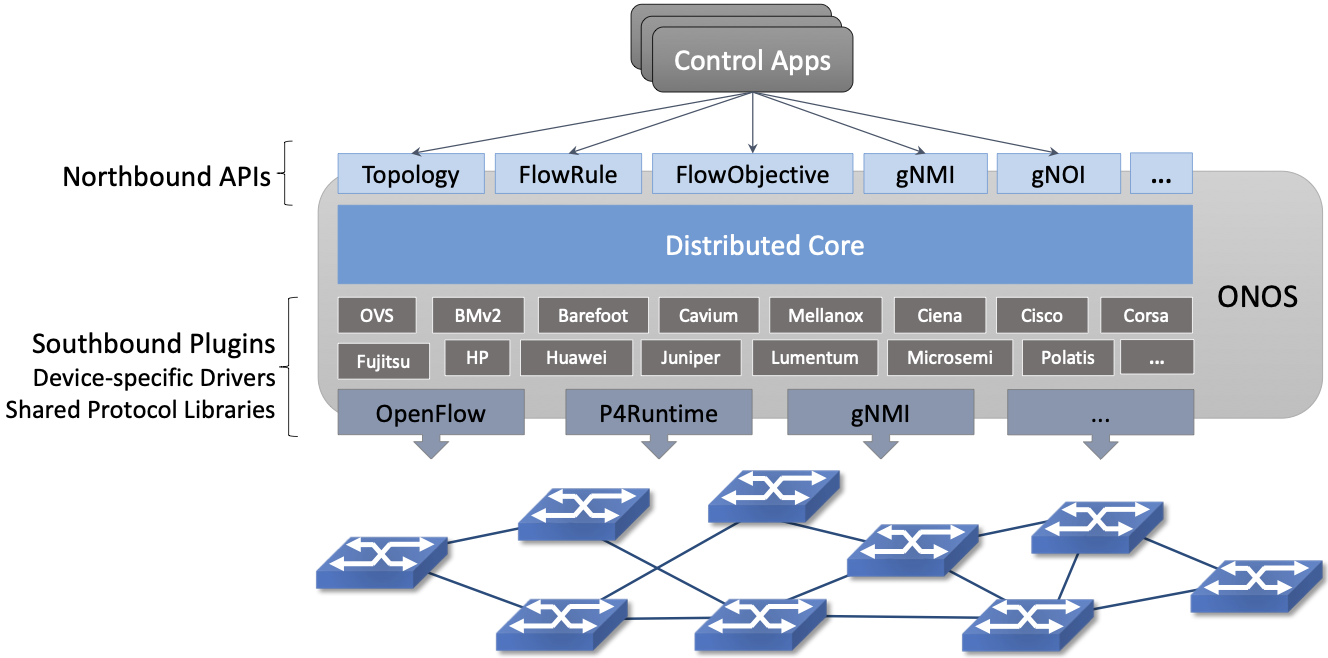
\includegraphics[width=\textwidth]{archivos/img/teoria/onos.png}
    \caption{Arquitectura del controlador \glsentryshort{sdn} onos \cite{onos1}}
    \label{fig:onos}
\end{figure}

\gls{onos} cuenta con una comunidad activa de desarrolladores y usuarios que contribuyen al desarrollo y mejora del sistema. Además, \gls{onos} es utilizado en diversos casos de uso, como redes de transporte, redes de centros de datos y redes de telecomunicaciones, entre otros muchos casos de uso. Si bien es cierto que tiene un muy buen rendimiento, no es controlador sencillo de manejar, y la curva de aprendizaje puede ser bastante pronunciada.

%%%%%%%%%%%%%%%%%%%%%%%%%%%%%%%%%%%%%%%%%%%%%%%%%%%%%%%%%%%%%%%%%%%%%%%%%%%%%%%%%%%%%%%%%%%%%%%%%%%%%
% Switches OVS & BOFUSS
\section{Software Switches \glsentryshort{sdn}}
\label{sec:softSwitchs}

En las redes definidas por software, los software switches desempeñan un papel fundamental al permitir la virtualización y la gestión centralizada de las redes. Estos switches, a diferencia de los switches de hardware tradicionales, se implementan como software y se ejecutan en servidores convencionales. Un software switch en \gls{sdn}, en adelante \textit{softswitch}, es una entidad lógica que reside generalmente en una instancia virtual o en un servidor, y se comunica con el controlador \gls{sdn} para recibir instrucciones sobre cómo procesar los paquetes de datos que fluyen a través de la red. Al estar basados en software, estos switches pueden ser escalados y desplegados de manera flexible según las necesidades y demandas de la red. La principal ventaja de los \textit{softswitches} radica en su capacidad para adaptarse y responder de manera dinámica a las necesidades de la red. Pueden implementar diferentes funciones de red, como enrutamiento, conmutación, balanceo de carga y seguridad, a través de la instalación de reglas desde el controlador \gls{sdn}. \\
\\
% fig
\begin{figure}[ht]
    \centering
    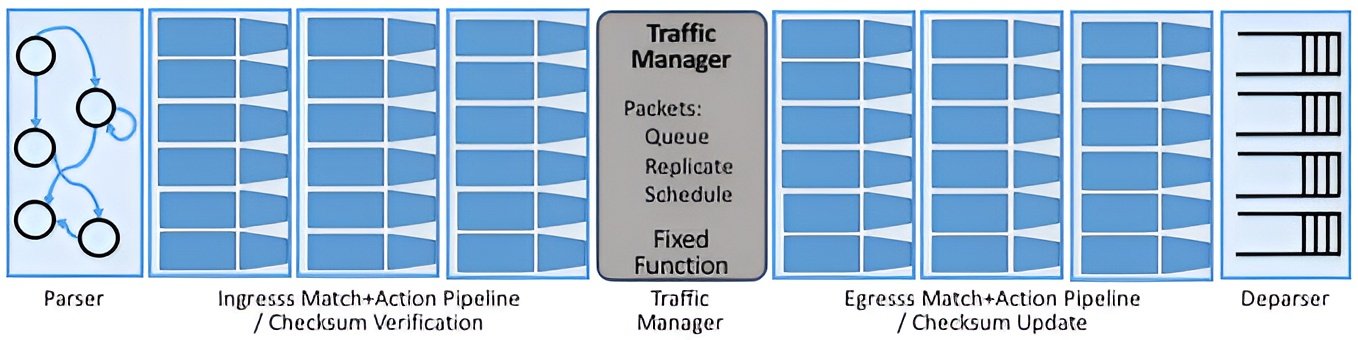
\includegraphics[width=0.8\textwidth]{archivos/img/teoria/softswitch.jpg}
    \caption{Arquitectura genérica de un \textit{softswitch} \gls{sdn} \cite{softswitches1}}
    \label{fig:softswitch}
\end{figure}

Según se puede apreciar en la figura \ref*{fig:softswitch}, la arquitectura genérica de un \textit{softswitch} se puede resumir en los siguientes bloques. El primero de todos tiene que ser un parser, que vaya inspeccionando los paquetes entrantes a la pipeline de procesamiento del switch para identificar que tipo es. Una vez se ha identificado el paquete que se va a procesar, el siguiente bloque son las tablas de \textit{match-action}, las cuales tienen una interfaz de comunicación con el controlador \gls{sdn} para establecer criterios y campos de \textit{match}, y en caso de haber un \textit{match}, definir una serie de acciones para llevar a cabo. En función del \textit{softswitch}, la verificación de \textit{checksum}\footnote{Suma de comprobación, campo para comprobar la integridad del paquete de datos} se puede llevar a cabo en el parser o en la etapa de las tablas de \textit{match-action}. El siguiente bloque que nos podemos encontrar en un \textit{softswitch} es el conocido como gestor de tráfico, que variará en función de la implementación, pero nos proveerá de gestión de colas, \gls{qos}, duplicado de paquetes, etc. La siguiente etapa ya es más opcional, que se suele denominar como \textit{egress match-action}, la cual se puede utilizar para definir algún tipo de lógica a la salida de los switches, aunque en la realidad se suele utilizar para actualizar los campos  de \texttt{TTL} y recalcular el \textit{checksum} dado que el paquete se habrá visto modificado. El último bloque es el deparser, el cual se encarga de ensamblar de nuevo el paquete y prepararlo para sacarlo por el puerto de salida del switch.

\subsection{OVS}
\label{subsec:OVS}

OVS (Open vSwitch) es un software switch de código abierto diseñado específicamente para su uso en redes definidas por software (SDN). Es uno de los software switches más utilizados y ampliamente adoptados en entornos SDN debido a su flexibilidad y funcionalidades avanzadas.

Open vSwitch actúa como un switch virtual, proporcionando capacidades de conmutación y enrutamiento para máquinas virtuales y contenedores en entornos de virtualización. Puede ejecutarse en hipervisores populares, como KVM (Kernel-based Virtual Machine), Xen y VMware, y también puede ser implementado como un switch independiente en sistemas operativos de servidor.

Las características clave de Open vSwitch incluyen:

1. Controlador SDN: Open vSwitch se puede controlar y programar mediante un controlador SDN, como OpenDaylight o ONOS. Esto permite una gestión centralizada y un control más granular de la red, así como la implementación de políticas de red definidas por software.

2. Funcionalidades avanzadas: OVS ofrece una amplia gama de funcionalidades, como enrutamiento, balanceo de carga, aislamiento de red, seguridad y calidad de servicio (QoS). Estas características permiten una gestión eficiente de la red y la implementación de políticas específicas para satisfacer las necesidades de las aplicaciones y usuarios.

3. Segmentación de red: Open vSwitch es compatible con la segmentación de red, lo que permite la creación de redes virtuales (network slices) dentro de una infraestructura compartida. Esto permite el aislamiento y la asignación de recursos personalizados para diferentes aplicaciones o usuarios, mejorando la seguridad y el rendimiento de la red.

4. Integración con tecnologías de virtualización: OVS se integra estrechamente con tecnologías de virtualización como OpenStack y Docker. Puede proporcionar conectividad de red entre máquinas virtuales, contenedores y hosts físicos, facilitando la migración y la gestión de recursos en entornos virtualizados.

5. Extensibilidad y soporte para estándares: Open vSwitch es altamente extensible y se puede ampliar mediante la integración de módulos y complementos personalizados. Además, cumple con los estándares de la industria, como el protocolo OpenFlow, para garantizar la interoperabilidad con otros componentes SDN.

En resumen, Open vSwitch (OVS) es un software switch SDN ampliamente utilizado que proporciona capacidades avanzadas de conmutación y enrutamiento para entornos de virtualización. Su flexibilidad, funcionalidades avanzadas, segmentación de red y compatibilidad con estándares lo convierten en una opción popular para implementaciones SDN en diversos entornos, desde centros de datos hasta infraestructuras de proveedores de servicios.

\subsection{BOFUSS}
\label{subsec:BOFUSS}

%%%%%%%%%%%%%%%%%%%%%%%%%%%%%%%%%%%%%%%%%%%%%%%%%%%%%%%%%%%%%%%%%%%%%%%%%%%%%%%%%%%%%%%%%%%%%%%%%%%%%
% Contiki-ng
\section{Contiki-ng}
\label{sec:contikiNG}

Contiki es un sistema operativo diseñado específicamente para dispositivos de baja capacidad, como sensores. Fue desarrollado por Adam Dunkels en colaboración con Bjorn Gronvall y Thiemo Voigt en 2002. A lo largo de los años, el proyecto Contiki ha crecido enormemente y ha involucrado a numerosas empresas y cientos de colaboradores en su repositorio de GitHub\footnote{\url{https://github.com/contiki-os/contiki}}. El objetivo principal de Contiki era proporcionar a los nodos de las redes de sensores inalámbricos (WSN) un sistema operativo liviano capaz de cargar y descargar servicios de forma dinámica \cite{1367266}.\\
\\
El kernel de Contiki se basa en un modelo orientado a eventos y admite multitarea con prelación. Está escrito en lenguaje C y ha sido portado a diversas arquitecturas de microcontroladores, como el MSP430 de Texas Instruments y sus variantes.\\
\\
En un sistema que ejecuta Contiki, este se divide en dos partes claramente diferenciadas, como se muestra en la Figura \ref{fig:contikiParts}: el núcleo (\textit{core}) y los programas o servicios cargados. Esta partición se realiza durante la etapa de compilación y es independiente del objetivo (target) donde se desplegará el sistema. El núcleo (\textit{core}) incluye el propio kernel, un conjunto de servicios base (como temporizadores y controladores), bibliotecas, controladores y el stack de comunicación. Los programas o servicios cargados se mapean en memoria mediante el cargador del kernel durante el tiempo de ejecución.\\


% Foto 
\begin{figure}[ht]
    \centering
    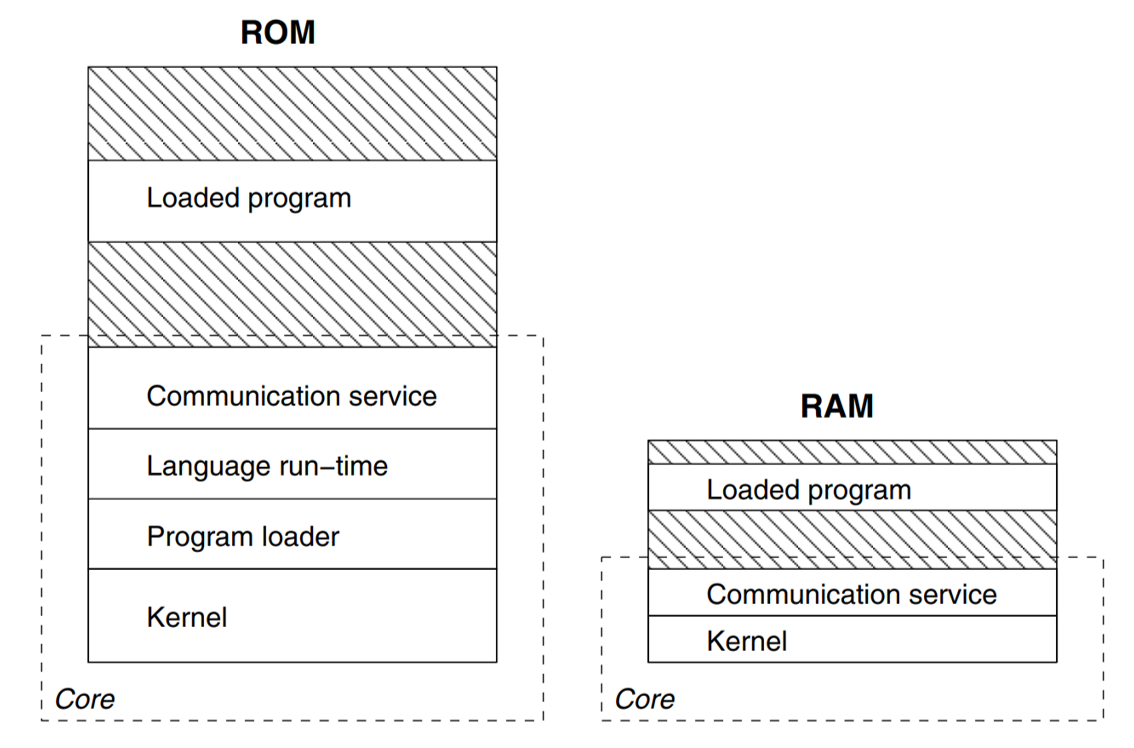
\includegraphics[width=0.8\textwidth]{archivos/img/teoria/contiki.png}
    \caption{Gestión de la memoria en un sistema con Contiki OS \cite{1367266}}
    \label{fig:contikiParts}
\end{figure}


En los últimos años ha surgido un nuevo proyecto llamado \textbf{Contiki-ng}\footnote{\url{https://github.com/contiki-ng/contiki-ng}}, el cual es un fork del sistema operativo Contiki. Este proyecto ha ganado popularidad y ha superado a su predecesor con el eslogan ``Contiki-NG: El sistema operativo para dispositivos IoT de próxima generación". Actualmente, toda la comunidad de Contiki se está centrando en este nuevo proyecto, el cual proporciona un stack de comunicación más compatible con las especificaciones RFC, ofrece soporte para protocolos como IPv6/6LoWPAN y 6TiSCH, y se está volviendo cada vez más popular por su capacidad de brindar soporte a microcontroladores con arquitectura ARM \cite{kurniawan2018practical}.

\subsection{Simulador Cooja}

El flujo de trabajo con Contiki o Contiki-ng varía dependiendo de si se trabaja con hardware real o si se realiza una simulación de los programas desarrollados. En el caso de trabajar con hardware real, el proceso consiste en compilar el sistema operativo y los programas específicos utilizando el objetivo (target) correspondiente, lo que generará un archivo binario que se puede cargar en la memoria del hardware.\\
\\
Por otro lado, si se opta por la simulación, se utilizará el simulador llamado Cooja\footnote{\url{https://github.com/contiki-ng/cooja/tree/master}}. Cooja es un simulador escrito en Java que permite \textbf{simular} una serie de nodos \gls{iot}. Al simular, es posible observar el comportamiento del programa desarrollado en diferentes plataformas. El proceso de compilación del núcleo (core) de Contiki y los programas desarrollados está integrado en el propio simulador, lo que facilita al usuario la compilación de sus programas para diferentes tipos de nodos. Cada simulación se puede guardar en un archivo con extensión \texttt{*.csc}, que almacena todos los datos de la simulación, como la semilla (\textit{seed}), las posiciones y los tipos de nodos, utilizando una estructura XML.\\
\\
De esta manera, tanto si se trabaja con hardware real como si se realiza una simulación, Contiki y Contiki-ng ofrecen herramientas y entornos integrados que permiten desarrollar y probar programas para sistemas embebidos y dispositivos \gls{iot}. A continuación, en la figura \ref{fig:cooja}, se indica la interfaz gráfica del simulador.

\begin{figure}[ht]
    \centering
    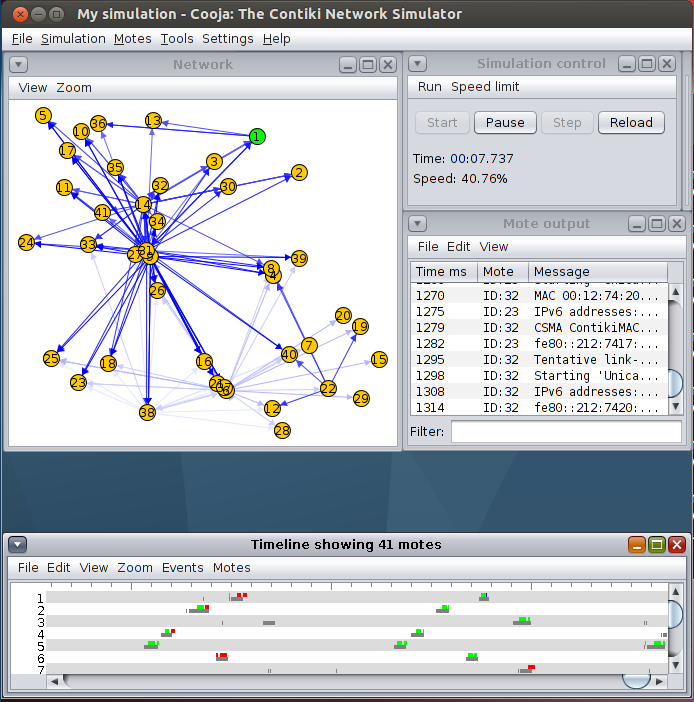
\includegraphics[width=0.6\textwidth]{archivos/img/teoria/cooja.png}
    \caption{Interfaz gráfica del simulador Cooja \cite{cooja1}}
    \label{fig:cooja}
\end{figure}



%%%%%%%%%%%%%%%%%%%%%%%%%%%%%%%%%%%%%%%%%%%%%%%%%%%%%%%%%%%%%%%%%%%%%%%%%%%%%%%%%%%%%%%%%%%%%%%%%%%%%
% Contribuciones en repos - Github
\section{Contribuciones en GitHub}
\label{sec:estadoArte_github}


El proyecto GitHub es una plataforma que proporciona alojamiento de repositorios. En el presente Trabajo de Fin de Máster (TFM), se utilizará la herramienta de control de versiones Git\footnote{\url{https://git-scm.com/}}, junto con GitHub como plataforma para alojar el código desarrollado. Sin embargo, GitHub no se utilizará únicamente para almacenar el código del TFM, sino que se aprovechará su carácter público para ofrecer documentación y ejemplos a todos los usuarios interesados que visiten el repositorio. \\
\par
\begin{itemize}
    \item Enlace al repositorio del \gls{tfm}: \url{https://github.com/davidcawork/TFM}
    \item Enlace al repositorio de la tesis: \url{https://github.com/davidcawork/tfm-thesis}
\end{itemize}
\vspace{0.5cm}

El repositorio incluye ficheros \texttt{README.md} en todos los directorios, que proporcionan explicaciones y análisis teóricos que permiten al visitante comprender la naturaleza de las pruebas, sus objetivos y las conclusiones que se pueden extraer de ellas. El propósito del repositorio es doble, ya que no solo almacena el código, sino que también ayuda a difundir los contenidos del proyecto. Además, se han ofrecido contribuciones útiles que pueden beneficiar a otros repositorios a través de solicitudes de extracción (pull requests). Durante este proyecto se ha contribuido de forma muy activa en varios proyectos opensource dado que la naturaleza del mismo abarcaba varias herramientas.  La tabla \ref{tab:githubContr} muestra todas las contribuciones realizadas.\\
\\

\begin{table}[ht]
    \centering
    \resizebox{\textwidth}{!}{%
        \begin{tabular}{|l|l|}
            \hline
            \rowcolor[HTML]{EFEFEF}
            \multicolumn{1}{|c|}{\cellcolor[HTML]{EFEFEF}{\color[HTML]{24292E} \textbf{Contribución}}} & \multicolumn{1}{c|}{\cellcolor[HTML]{EFEFEF}{\color[HTML]{24292E} \textbf{Enlace al Pull-Request}}} \\ \hline
            Dar soporte al bmv2 entorno P4 en Mininet-WiFi                                             & \url{https://github.com/intrig-unicamp/mininet-wifi/pull/302}                                       \\ \hline
            Arreglar la compilación del BOFUSS en Mininet-WiFi                                         & \url{https://github.com/intrig-unicamp/mininet-wifi/pull/495}                                       \\ \hline
            Aclarar el uso de ONOS-gui                                                                 & \url{https://groups.google.com/a/opennetworking.org/g/onos-dev/c/mbfyCaoeCdU}                       \\ \hline
            Resolver problema interfaz dpctl con el BOFUSS                                             & \url{https://github.com/mininet/mininet/issues/745}                                                 \\ \hline
            Dar escenarios funcionales en la 22.04 de Mininet con Onos                                 & \url{https://groups.google.com/a/opennetworking.org/g/onos-dev/c/a0VjA0Xw_-M}                       \\ \hline
        \end{tabular}%
    }
    \caption{Resumen de contribuciones realizadas durante todo el proyecto del \gls{tfm}}
    \label{tab:githubContr}
\end{table}

%\chapter{Diseño del protocolo de control In-Band}
\label{ch:analisis}

En este capítulo, se abordará una fase fundamental del proyecto, centrada en el diseño de un protocolo de control In-Band para la gestión de redes. En este capítulo, se realizará un exhaustivo análisis de soluciones anteriores basadas en el enfoque In-Band, donde se explorarán diferentes propuestas y se evaluarán sus fortalezas y debilidades.\\
\\
El objetivo principal será definir las funcionalidades básicas que debe poseer el protocolo de control In-Band, considerando los requisitos específicos del proyecto y las necesidades de los entornos de redes actuales. Se examinarán aspectos clave, como la capacidad de establecer una conexión entre los nodos de la red y el controlador, el manejo eficiente del plano de datos para la transmisión de información de control y la escalabilidad para adaptarse a entornos de redes heterogéneas y de gran tamaño. Además, se proporcionará una explicación detallada del funcionamiento del protocolo diseñado, describiendo los diferentes componentes, los mensajes intercambiados entre nodos y controlador, así como los procedimientos de configuración y gestión de la red. Se analizarán las decisiones de diseño tomadas y se justificarán en base a los objetivos del proyecto y las características de los entornos de redes abordados.Por último, se tomará una decisión sobre la plataforma más adecuada para la implementación del protocolo de control In-Band. Se evaluarán diferentes opciones, considerando factores como la disponibilidad de herramientas y tecnologías relevantes, la compatibilidad con los requisitos del proyecto y la viabilidad de su implementación en entornos reales.

%%%%%%%%%%%%%%%%%%%%%%%%%%%%%%%%%%%%%%%%%%%%%%%%%%%%%%%%%%%%%%%%%%%%%%%%%%%%%%%%%%%%%%%%%%%%%%%%%
\section{Protocolo In-Band}
\label{sec:ana_inband}

iotorii hackmd

%%%%%%%%%%%%%%%%%%%%%%%%%%%%%%%%%%%%%%%%%%%%%%%%%%%%%%%%%%%%%%%%%%%%%%%%%%%%%%%%%%%%%%%%%%%%%%%%%
\section{Plataforma de desarrollo y validación}
\label{sec:ana_mininet_wifi}

blabla bla contikiwith cooja vs mininet wifi (sim vs emu )

%%%%%%%%%%%%%%%%%%%%%%%%%%%%%%%%%%%%%%%%%%%%%%%%%%%%%%%%%%%%%%%%%%%%%%%%%%%%%%%%%%%%%%%%%%%%%%%%%
\section{Agente \glsentryshort{sdn}}
\label{sec:ana_switch}

why bofuss ? i mean, we have already an implementation of inband on it

\dots

%%%%%%%%%%%%%%%%%%%%%%%%%%%%%%%%%%%%%%%%%%%%%%%%%%%%%%%%%%%%%%%%%%%%%%%%%%%%%%%%%%%%%%%%%%%%%%%%%
\section{Agente de control \glsentryshort{sdn}}
\label{sec:ana_controller}

En este punto se tiene que valorar qué agente de control \gls{sdn}, es decir controlador \gls{sdn} se va a utilizar. Se tendrán en cuenta las condiciones del entorno sobre el cual se va a desplegar, así como las características propias de cada controlador, así como la facilidad y flexibilidad que nos entregue cada uno para desplegarlo sobre la plataforma emulada. Las opciones que se han considerado para este cometido son las siguientes:

\begin{itemize}
    \item Ryu, explicado anteriormente en la sección \ref{subsec:ryu} del estado del arte.

    \item \gls{onos}, explicado anteriormente en la sección \ref{subsec:ONOS} del estado del arte.
\end{itemize}

Según se ha explicado ya, cada herramienta tiene sus puntos fuertes y sus puntos debiles, por lo que vamos a realizar una comparativa para nuestro caso de uso para ver cual de las dos nos interasa mś utilizar para este proyecto.

\begin{itemize}
    \item El controlador ONOS es más potente que Ryu, es utilizado generalmente por los operadores de red, y es conocido por su rendimiento y su solided.
    \item El controlador ONOS tiene un rendimiento superior a Ryu en terminos de procesamiento de paquetes.
    \item El controlador Ryu sin embargo, pesa menos, y es más sencillo de depurarle y meter nuevas funcionalidades si es necesario.
    \item El controlador Ryu al pesar menos, tambien se despliega y se instala más rapido frente al controlador de ONOS.
    \item Al ser más Ryu más pequeño, la curva de aprendizaje de ryu frente a ONOS también es menor.
    \item Una cosa que sería una ventaja es que ONOS tiene descubrimiento topologico con una interfaz web bastante fancy que nos ayudaría a depurar el código desarrollado del protocolo, sin embargo, esta aplicación de descubrimiento topologico corre haciendo uso del protocolo \gls{lldp}, el cual no decubriría la configuración de los enlaces inalambricos, solo a los nodos, por lo que no seria de utilidad. Si bien es cierto que hay algunas publicaciones que si han contemplado esta necesidad, sería inviable poner a implementar dicho protocolo en el proyecto dado que se escaparía de los objetivos temporales y de alcance del proyecto.
\end{itemize}

%%%%%%%%%%%%%%%%%%%%%%%%%%%%%%%%%%%%%%%%%%%%%%%%%%%%%%%%%%%%%%%%%%%%%%%%%%%%%%%%%%%%%%%%%%%%%%%%%
\section{Análisis funcional de la interfaz del \glsentryshort{bofus}}
\label{sec:ana_bofuss}

En esta sección, exploraremos en detalle el análisis funcional de la interfaz del \gls{bofus}, centrándonos específicamente en los binarios que componen su arquitectura. Estos binarios, conocidos como \texttt{ofdatapath} y \texttt{ofprotocol}, desempeñan un papel fundamental en la operativa básica de este switch de espacio de usuario.\\
\\
El \texttt{ofdatapath}, como su nombre sugiere, es responsable de procesar el plano de datos en el \gls{bofus}. Este componente se encarga de recibir, analizar y tomar decisiones en función de los paquetes que atraviesan su pipeline de procesado de paquetes. A través del parser, tablas de flujo, y tablas de métricas, el ofdatapath garantiza una transferencia de datos fluida y eficiente en el entorno OpenFlow. Por otro lado, el \texttt{ofprotocol} se ocupa del agente de control en el \gls{bofus}. Su función principal consiste en establecer la comunicación entre el controlador y el switch. A través del \texttt{ofprotocol}, el controlador y \gls{bofus} pueden intercambiar información sobre el estado del switch, enviar nuevas reglas de procesado de paquetes, o recopilar estadísticas. Este binario es quien habilita al controlador llevar a cabo una gestión centralizada y dinámica de las políticas de red, facilitando la adaptación y optimización de la infraestructura según las necesidades del entorno.\\


\subsection{Binario \texttt{ofprotocol}}

El binario de ofprotocol establece un canal seguro de comunicación entre el \textit{datapath} OpenFlow y el controlador remoto. Este conecta con el plano de datos mediante Netlink o TCP, y con el controlador remoto mediante TCP o SSL, actuando de proxy entre los dos mundos. Se quiere señalar el hecho de que el binario pueda comunicarse con el \textit{datapath} mediante TCP, dado que según el creador de la herramienta indica que esos dos binarios pueden trabajar desacoplados en máquinas diferentes y comunicarse a través de la red. Sin embargo, esta configuración no es muy común, dado que la comunicación entre \textit{datapath} y agente de control es crítica, y no admiten ni delays, ni perdidas.\\


\begin{lstlisting}[language= bash, style=Consola, caption={Interfaz CLI del binario ofprotocol},label=code:binofproto]
    ofprotocol [options] datapath controller[,controller...]
\end{lstlisting}
\vspace{0.5cm}

Uno de los parámetros obligatorios a la hora de invocar al agente de control, es qué \textit{datapath} se va a gestionar. Este se puede indicar de las siguientes formas.

\begin{itemize}
    \item \texttt{unix:file}, se indica un descriptor de un socket UNIX, el cual deber ser el mismo que se indique a la hora que ejecute el ofdatapath. Mediante este socket unix se comunicarán \textit{datapath} y agente de control.

    \item \texttt{tcp:HOST[:PORT]}, en este caso, también se puede conectar en red mediante puerto y dirección IP. Este tipo de identificación se usa cuando se quiere tener separado en máquinas diferentes \textit{datapath} y agente de control. El puerto que se emplea por defecto es el 6653.
\end{itemize}

En cambio, el parámetro del controlador es opcional, y solo soporta conexiones TCP. Para la conexión con el controlador se contemplan dos paradigmas diferentes para la conexión del controlador.

\begin{itemize}
    \item \texttt{out-of-band}: con esta configuración el tráfico OpenFlow utiliza una red privada para comunicarse con el controlador.

    \item \texttt{in-band}: con esta configuración el tráfico OpenFlow viaja por la misma red que la red de datos. Esta opción es la opción por defecto.
\end{itemize}

Para llevar a cabo la configuración manual del control in-band, es necesario realizar algunos pasos clave con antelación. En primer lugar, se requiere especificar la ubicación precisa del controlador al llamar al binario de ofprotocol. Esto asegurará una conexión adecuada entre el controlador y el agente de control. Además, es crucial configurar la interfaz de red como el puerto local OpenFlow, el cual permite que ofprotocol establezca una conexión efectiva con el controlador. El puerto local OpenFlow es un puerto de red virtual que actúa como puente entre los puertos físicos del switch y el controlador. Para lograr esto, se puede especificar el nombre de la interfaz de red asignada al puerto local mediante la opción \texttt{--local-port} en la línea de comandos del binario ofdatapath. Generalmente, si no se indica ninguna interfaz, será el propio binario quien genere una interfaz de tipo TUN/TAP con el nombre \texttt{tap0/tun0}. Siguiendo estos pasos, se puede configurar adecuadamente el control in-band.


\subsection{Binario \texttt{ofdatapath}}


La herramienta de ofdatapath representa una valiosa implementación en el ámbito de las datapaths OpenFlow. Esta herramienta, diseñada para funcionar en el espacio de usuario, tiene la capacidad de supervisar y gestionar una o más interfaces de red de manera eficiente. Estas interfaces actúan como canales de comunicación fundamentales a través de los cuales los paquetes de datos son transmitidos y reenviados según las políticas y reglas establecidas en las tablas de flujos (Ir a sección \ref{subsec:BOFUSS}). Gracias a esta funcionalidad, ofdatapath permite un control efectivo y granular a nivel de flujo de datos en la red, asegurando un enrutamiento adecuado y optimizado de los paquetes. Su flexibilidad y adaptabilidad a diferentes escenarios hacen de esta herramienta una elección preferida en entornos OpenFlow a la hora de hacer pruebas de concepto, donde se busca una implementación amigable y funcional de un agente OpenFlow. A continuación en el bloque de código \ref{code:binofdata} se indica la interfaz de comandos de este bibario.\\

\begin{lstlisting}[language= bash, style=Consola, caption={Interfaz CLI del binario ofdatapath},label=code:binofdata]
    ofprotocol [options] datapath controller[,controller...]
\end{lstlisting}
\vspace{0.5cm}

La combinación del binario ofdatapath junto con el binario ofprotocol da lugar a lo que se conoce como \gls{bofus} (Basic OpenFlow Software Switch), una solución integral de software switch \gls{sdn} OpenFlow. Al utilizar \gls{bofus}, se obtiene un control y gestión a bajo nivel de las interfaces de red, lo que permite una administración eficiente de los flujos de datos que atraviesan la pipeline de procesamiento del switch. Es importante destacar que, para acceder a estas interfaces de red, el binario generalmente requiere ejecutarse con privilegios de super usuario. Además, es relevante considerar la forma en la que estos binarios se comunican entre sí. Por lo general, esta comunicación se establece a través de un socket UNIX, permitiendo una conexión directa y eficiente entre ambos componentes. Sin embargo, también es posible establecer una conexión pasiva mediante TCP, ofreciendo una alternativa para la comunicación entre los binarios. Esta flexibilidad en los mecanismos de comunicación brinda opciones adaptativas y versátiles, permitiendo que \gls{bofus} se adapte a diferentes entornos y necesidades. \\
\\
A continuación, se indican algunos de los parámetros más importantes de la interfaz CLI del binario ofdatapath. Empezando por el único de ellos obligatorio, que es, cómo indicamos el punto de comunicación del plano de datos hacia el exterior, véase un agente de control, como por ejemplo el binario ofprotocol.\\

\begin{itemize}
    \item \texttt{punix:file}, escucha por una conexión en el descriptor del socket UNIX indicado.

    \item \texttt{ptcp:[port]}, escucha por conexiones TCP en el puerto determinado. Según la wiki de la herramienta, indican que el puerto por defecto es el 975, lo que en la práctica no es verdad\footnote{Se tuvo que modificar la wiki de la herramienta \url{https://github.com/CPqD/ofsoftswitch13/wiki/Ofdatapath-Manual/_history}}, es el 6653.
\end{itemize}

El valor del puerto por defecto se puede comprobar fácilmente, a continuación en las figuras \ref{fig:ofdata_1} y \ref{fig:ofdata_2}. Como se puede ver se lanza el binario de forma \textit{standalone} sobre la interfaz de loopback del sistema, y si comprobamos con la herramienta \texttt{lsof} los puertos TCP en esto de escucha en la Network namespace por defecto, se puede ver como el binario está utilizando el puerto 6653. Pero se puede ir un paso más allá, podemos ir al propio código fuente de la herramienta, y ver en que macro definen el puerto por defecto, lo cual se puede comprobar \href{https://github.com/CPqD/ofsoftswitch13/blob/master/include/openflow/openflow.h#LL75C1-L75C27}{aquí}.

%fig 1
\begin{figure}[ht]
    \centering
    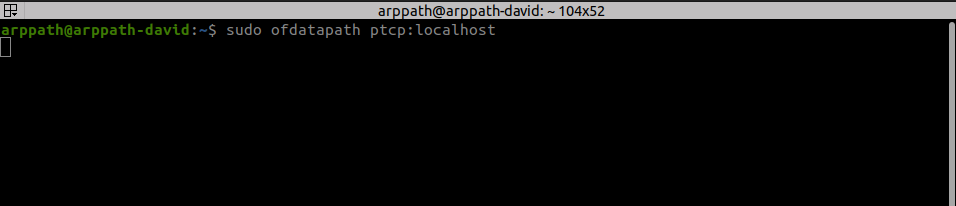
\includegraphics[width=\textwidth]{archivos/img/analisis/ofdata_1.png}
    \caption{Ejecución del binario \texttt{ofdatapath} en modo standalone}
    \label{fig:ofdata_1}
\end{figure}

%fig 2
\begin{figure}[ht]
    \centering
    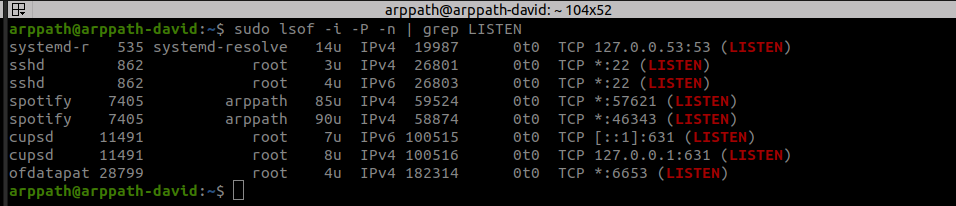
\includegraphics[width=\textwidth]{archivos/img/analisis/ofdata_2.png}
    \caption{Comprobación del puerto de  escucha del binario \texttt{ofdatapath}}
    \label{fig:ofdata_2}
\end{figure}


Sigamos con los parámetros de configuración del software switch. Uno de los más importantes, es indicar los puertos a gestionar el switch. Es decir, que interfaces va a manejar.

\begin{itemize}
    \item \texttt{-i, --interfaces=netdev[,netdev]}, Con este comando indicamos cada puerto que tendrá el switch. Cada interfaz se le asignará un número de puerto. Otro, detalle a tener en cuenta es que las interfaces no pueden tener IPs.

    \item \texttt{-L, --local-port=netdev}, Con este comando indicamos el puerto local que tendrá el switch el cual será la interfaz física o virtual, que se usará para el control in-band. Cuando está opción no está indicada, por defecto, se creará una interfaz de tipo tap, tap0 o algo así, la cual se utilizará para el control del software switch. Si no se quiere dejar como responsabilidad al Kernel la de asignar un nombre a la interfaz tap, se puede indicar como \texttt{--local-port=tap:name}. Se crea aquí. Para más información sobre las interfaces tun/tap, ver la sección \ref{linuxNetworking_tuntap}.

    \item \texttt{--no-local-port}, se le indica al software switch que no va a utilizar un puerto local, ergo, no podremos trabajar en modo in-band.

    \item \texttt{--no-slicing}, se utiliza para deshabilitar la configuración de las colas asociadas a los puertos. Por ello, contendrá un total de 0 colas. Esta opción se suele utilizar cuando algunas de las configuraciones de colas (tc y kernel) no se encuentran disponibles. (Mininet y Mininet-wifi corre el BOFUSS con esta opción por defecto).

    \item \texttt{-d, --datapath-id=dpid}, Especifica el Datapath ID Openflow, conocido como dpid. Es un identificador del datapath de 16 dígitos hexadecimales. Si no se especifica, el ofdatapath pilla uno aleatorio.
\end{itemize}

%%%%%%%%%%%%%%%%%%%%%%%%%%%%%%%%%%%%%%%%%%%%%%%%%%%%%%%%%%%%%%%%%%%%%%%%%%%%%%%%%%%%%%%%%%%%%%%%%
\section{Análisis de la clase \texttt{UserAP} en Mininet-WiFi}
\label{sec:ana_userap}

En esta sección, vamos a sumergirnos en un análisis exhaustivo de la clase \texttt{UserAP} en Mininet-WiFi, una pieza fundamental que envuelve al \gls{bofus}. Al observar detenidamente el diagrama UML de clases en la figura \ref{fig:userAP}, nos encontramos con una intrigante jerarquía de clases relacionadas con \texttt{UserAP}. En el centro de esta estructura se encuentran las clases primigenias, \texttt{Node} y \texttt{Node\_wifi}, que se llevan la mayor carga lógica al albergar la mayoría de atributos y métodos esenciales. Estas clases primigenias desempeñan un papel crucial al gestionar una serie de operaciones vitales. Entre sus responsabilidades se encuentran la creación de \textit{Network namespaces}, la configuración y creación de interfaces inalámbricas, el manejo del \gls{tc} para establecer los atributos de los enlaces y mucho más. Son el núcleo de la implementación que permite el funcionamiento armonioso de la infraestructura.\\
\\
No obstante, es importante destacar que la clase \texttt{UserAP}, encargada de encapsular al \gls{bofus}, también aporta su propia lógica especializada. Su tarea principal radica en la gestión del proceso \texttt{HostAPd}, un daemon que trabaja incansablemente para materializar las diversas funcionalidades de punto de acceso. Este componente es fundamental para dotar de vida y dinamismo a la red inalámbrica emulada. Además de su papel esencial en el despliegue del \gls{bofus}, estas clases tienen una responsabilidad adicional: implementar una interfaz de ejecución que permite adaptar las condiciones del escenario a los parámetros necesarios de la interfaz de línea de comandos del software switch \gls{sdn}. Esta adaptabilidad se convierte en una ventaja estratégica, ya que proporciona la flexibilidad necesaria para personalizar y ajustar el entorno según las necesidades específicas de cada caso de uso.
\newpage
% fig
\begin{figure}[ht!]
    \centering
    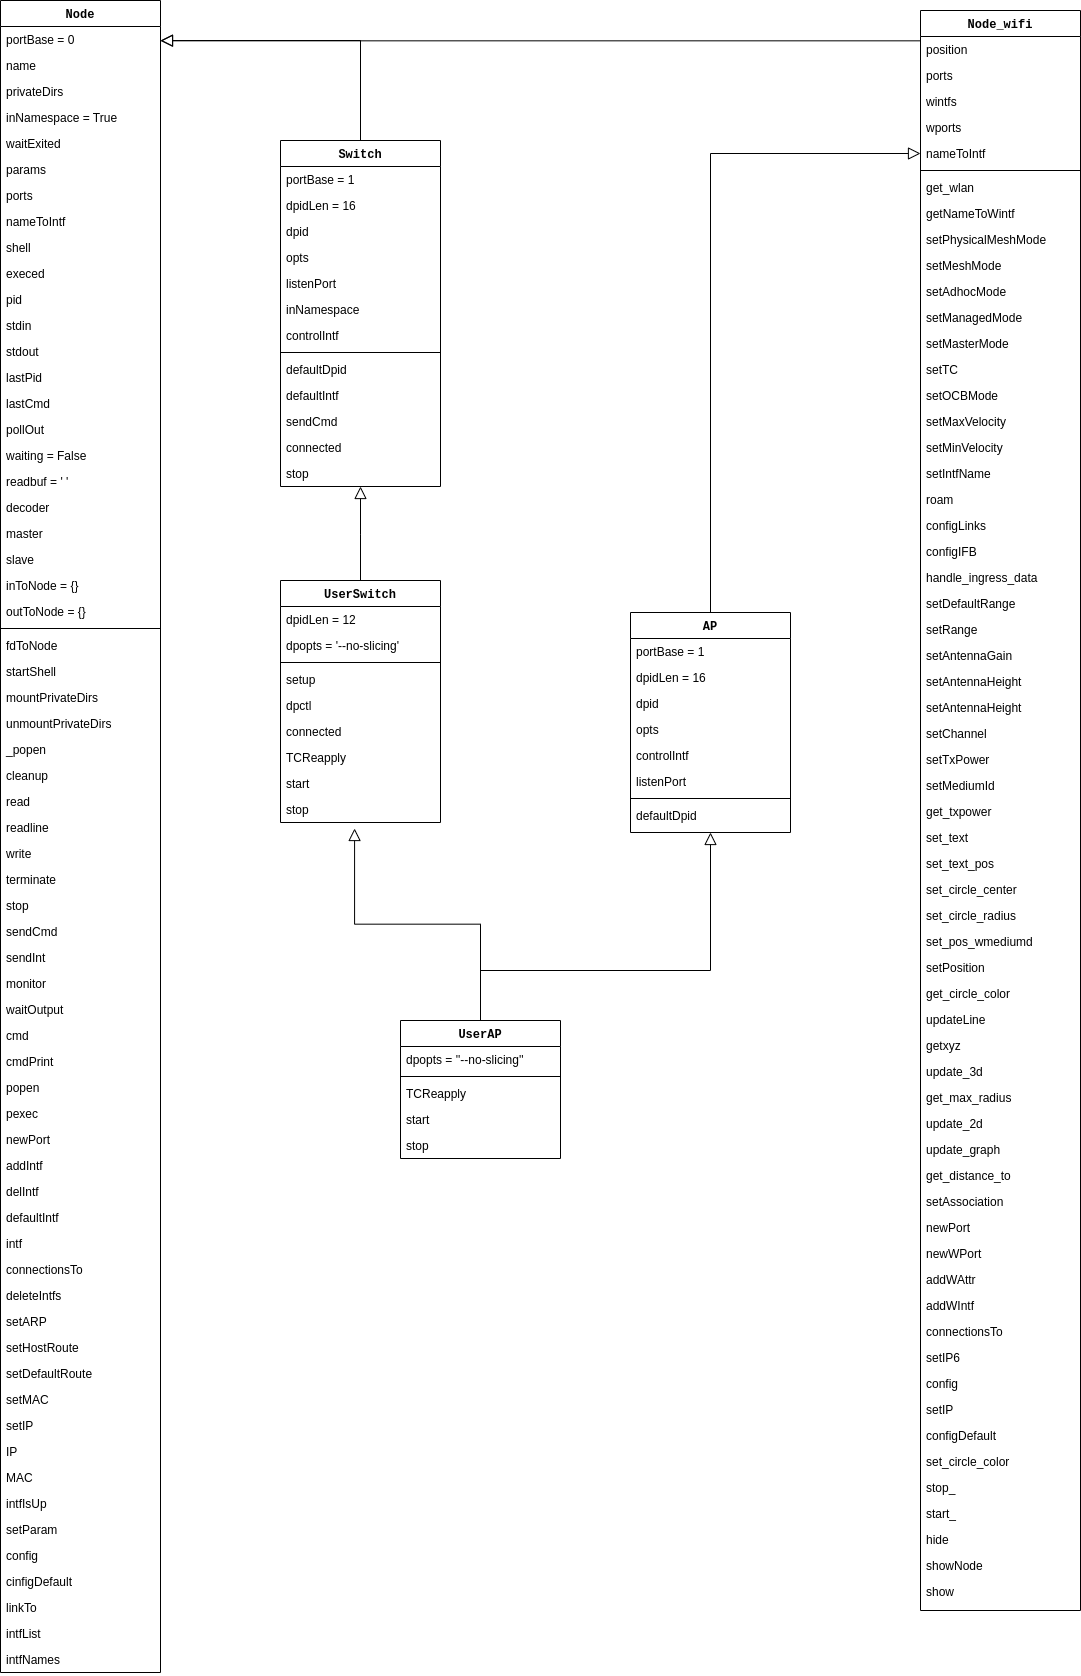
\includegraphics[width=0.8\textwidth]{archivos/img/analisis/userAP.png}
    \caption{Diagrama UML de la clase \texttt{UserAP}}
    \label{fig:userAP}
\end{figure}

Mencionar, que Mininet-Wifi redefine atributos que ya se encuentran en Mininet, como por ejemplo la longitud del identificador del \textit{datapath}. Muchos de los bugs encontrados entre los repositorios de las plataformas de emulación y el \gls{bofus}, se debe a incoherencias en la definición de las interfaces y a redefiniciones de parámetros como se ha podido encontrar. Por ello, para ver a bajo nivel como se ejecuta los binarios pertenecientes al \gls{bofus} se va a hacer una prueba de concepto lanzando una topología sencilla, y se va a estudiar las trazas de ejecución del mismo. Esto nos será de utilidad para poder comprender que comandos y llamadas al sistema se llevan a cabo para levantar una instancia de un software switch \gls{bofus}.\\
\\
La topología que se va a desplegar se puede apreciar en la figura \ref{fig:topoBasic}. Para lanzar dicha topología se tiene que lanzar un script de Python el cual se puede encontrar en el repositorio del \gls{tfm} (Sección \ref{sec:estadoArte_github}). A la par que se ejecuta el script de python que alberga la topología, se tiene que lanzar un controlador \gls{sdn} que le permita al software switch manejar correctamente los paquetes que atraviesen su \textit{datapath}. A continuación, en el bloque de código \ref{code:topoBasic}, se puede apreciar qué comandos se tienen que utilizar para  desplegar el escenario. \\

\begin{lstlisting}[language= bash, style=Consola, caption={Puesta en marcha del escenario básico},label=code:topoBasic]
    # Lanzamos el script que pone en marcha el medio inalambrico via Mininet-WiFi
    sudo python3 topo.py
   
    # Lanzamos el controlador (en otra terminal)
    ryu-manager ryu.app.simple_switch_13
\end{lstlisting}
\vspace{0.5cm}

Algún lector podría preguntarse en este punto como va a llevar se a cabo la comunicación entre el controlador \gls{sdn} y el \gls{bofus}. Dicha comunicación se producirá a través de la interfaz de red de \textit{loopback} de la Network namespace por defecto, donde el controlador de ryu estará escuchando en el puerto 6633, con una interfaz virtual de tipo \textit{tun} generada por el \gls{bofus} para llevar a cabo la conexión Openflow.  Para recolectar información sobre la traza de ejecución del script en Mininet-WiFi se debe poner el nivel de log a \textit{debug}.\\
\\

\begin{figure}[ht!]
    \centering
    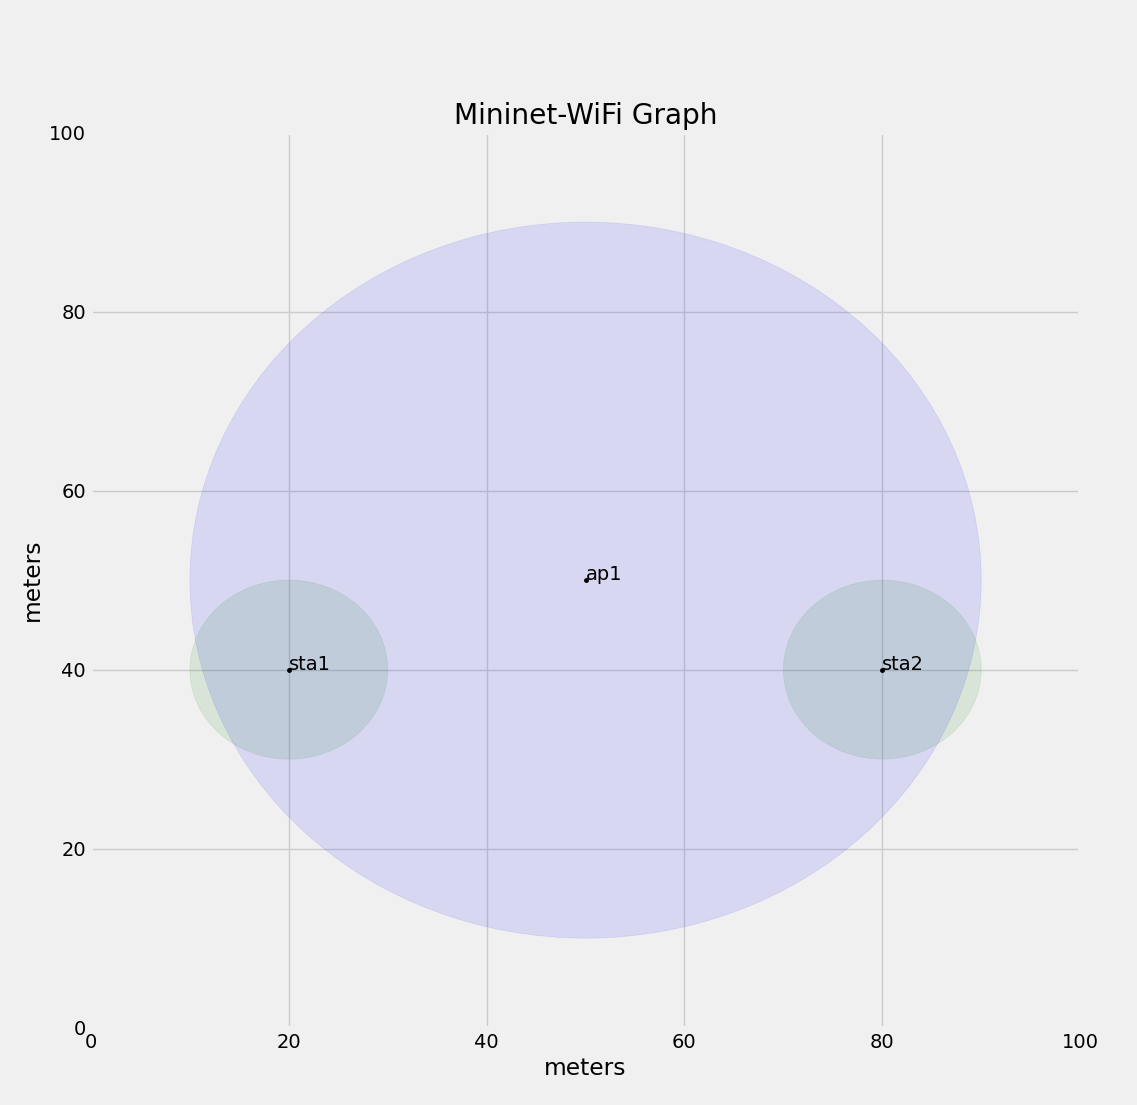
\includegraphics[width=0.7\textwidth]{archivos/img/analisis/topoBasic.png}
    \caption{Topología básica haciendo uso del \texttt{UserAP} (\gls{bofus})}
    \label{fig:topoBasic}
\end{figure}


A continuación, en el bloque de código \ref{code:trazatopobasic}, se puede apreciar la traza de ejecución de la topología básica. Dicha traza se ha limpiado y se han marcado las partes más importantes. Como se indicó anteriormente, esta traza es muy enriquecedora dado que nos permitirá a posteriori hacer nuestros propios escenarios a medida con topologías inalámbricas a bajo nivel. A lo largo de la traza, se podrán encontrar comentarios en verde que indican que operativas se están llevando a cabo en que parte.\\
\\

\begin{lstlisting}[language= bash, style=Consola, caption={Traza de la puesta en marcha del escenario básico},label=code:trazatopobasic]
    ### Primero se comprueba las caracteristicas del sistema sobre donde va a correr
    *** errRun: ['grep', '-c', 'processor', '/proc/cpuinfo'] 
    4
    0*** Setting resource limits
    *** Creating nodes
    *** Add Controller (Ryu) ***
    *** errRun: ['which', 'mnexec'] 
    /usr/bin/mnexec
    0*** errRun: ['which', 'ifconfig'] 
    /usr/sbin/ifconfig
    0_popen ['mnexec', '-cd', 'env', 'PS1=\x7f', 'bash', '--norc', '--noediting', '-is', 'mininet:c0'] 359891*** c0 : ('unset HISTFILE; stty -echo; set +m',)
    unset HISTFILE; stty -echo; set +m

    ### Se comprueba la conectividad con el controlador al puerto por defecto haciendole un telnet 
    *** c0 : ('echo A | telnet -e A localhost 6633',)
    Telnet escape character is 'A'.
    Trying 127.0.0.1...
    Connected to localhost.
    Escape character is 'A'.

    telnet> Connection closed.
    *** Add one UserAP ***
    *** errRun: ['which', 'mnexec'] 
    /usr/bin/mnexec
    0*** errRun: ['which', 'ip', 'addr'] 
    /usr/sbin/ip
    1_popen ['mnexec', '-cd', 'env', 'PS1=\x7f', 'bash', '--norc', '--noediting', '-is', 'mininet:ap1'] 359897*** ap1 : ('unset HISTFILE; stty -echo; set +m',)
    unset HISTFILE; stty -echo; set +m

    ### Se prepara el box del AP1 (El cual correrá el BOFUSS)
    added intf lo (0) to node ap1
    *** ap1 : ('ifconfig', 'lo', 'up')
    *** errRun: ['which', 'ofdatapath'] 
    /usr/local/bin/ofdatapath
    0*** errRun: ['which', 'ofprotocol'] 
    /usr/local/bin/ofprotocol

    ### Se prepara los boxes de las estaciones wifi
    *** Add two WiFi stations ***
    *** errRun: ['which', 'mnexec'] 
    /usr/bin/mnexec
    0*** errRun: ['which', 'ip', 'addr'] 
    /usr/sbin/ip
    1_popen ['mnexec', '-cdn', 'env', 'PS1=\x7f', 'bash', '--norc', '--noediting', '-is', 'mininet:sta1'] 359904*** sta1 : ('unset HISTFILE; stty -echo; set +m',)
    unset HISTFILE; stty -echo; set +m
    _popen ['mnexec', '-cdn', 'env', 'PS1=\x7f', 'bash', '--norc', '--noediting', '-is', 'mininet:sta2'] 359906*** sta2 : ('unset HISTFILE; stty -echo; set +m',)
    unset HISTFILE; stty -echo; set +m

    ### Se generan los radio taps emulados hacinedo uso del modulo del kernel mac80211_hwsim
    *** Configuring nodes
    Loading 3 virtual wifi interfaces
    Created mac80211_hwsim device with ID 0
    Created mac80211_hwsim device with ID 1
    Created mac80211_hwsim device with ID 2
    rfkill unblock 17

    ### Se cambian los nombres por defecto de las interfaces virtuales generadas a nombres 
    ### descriptivos que identifiquen a los nodos
    *** sta1 : ('ip link set wlan0 down',)
    *** sta1 : ('ip link set wlan0 name sta1-wlan0',)
    rfkill unblock 18
    *** sta2 : ('ip link set wlan1 down',)
    *** sta2 : ('ip link set wlan1 name sta2-wlan0',)
    *** ap1 : ('ip link set wlan2 down',)
    *** ap1 : ('ip link set wlan2 name ap1-wlan1',)
    *** ap1 : ('ip link set ap1-wlan1 up',)

    ### Se configura la interfaz virtual emulada wireless de la sta1
    added intf sta1-wlan0 (0) to node sta1
    *** sta1 : ('ip link set', 'sta1-wlan0', 'down')
    *** sta1 : ('ip link set', 'sta1-wlan0', 'address', '00:00:00:00:00:02')
    *** sta1 : ('ip link set', 'sta1-wlan0', 'up')
    *** sta1 : ('ip addr flush ', 'sta1-wlan0')
    *** sta1 : ('ip addr add 10.0.0.1/8 brd + dev sta1-wlan0 && ip -6 addr add 2001:0:0:0:0:0:0:1/64 dev sta1-wlan0',)
    *** sta1 : ('ip -6 addr flush ', 'sta1-wlan0')
    *** sta1 : ('ip -6 addr add', '2001:0:0:0:0:0:0:1/64', 'dev', 'sta1-wlan0')
    *** sta1 : ('ip link set lo up',)

    ### Se configura la interfaz virtual emulada wireless de la sta2
    added intf sta2-wlan0 (0) to node sta2
    *** sta2 : ('ip link set', 'sta2-wlan0', 'down')
    *** sta2 : ('ip link set', 'sta2-wlan0', 'address', '00:00:00:00:00:03')
    *** sta2 : ('ip link set', 'sta2-wlan0', 'up')
    *** sta2 : ('ip addr flush ', 'sta2-wlan0')
    *** sta2 : ('ip addr add 10.0.0.2/8 brd + dev sta2-wlan0 && ip -6 addr add 2001:0:0:0:0:0:0:2/64 dev sta2-wlan0',)
    *** sta2 : ('ip -6 addr flush ', 'sta2-wlan0')
    *** sta2 : ('ip -6 addr add', '2001:0:0:0:0:0:0:2/64', 'dev', 'sta2-wlan0')
    *** sta2 : ('ip link set lo up',)

    ### Se configura la interfaz virtual emulada wireless de la ap1 y el proceso
    ### de hostAPd
    added intf ap1-wlan1 (1) to node ap1
    *** ap1 : ('ip link set', 'ap1-wlan1', 'up')
    *** ap1 : ('ethtool -K', <WirelessLink ap1-wlan1>, 'gro', 'off')
    *** ap1 : ('ip link set', 'ap1-wlan1', 'down')
    *** ap1 : ('ip link set', 'ap1-wlan1', 'address', '00:00:00:00:00:01')
    *** ap1 : ('ip link set', 'ap1-wlan1', 'up')
    *** ap1 : ("echo 'interface=ap1-wlan1\ndriver=nl80211\nssid=new-ssid\nwds_sta=1\nhw_mode=g\nchannel=1\nctrl_interface=/var/run/hostapd\nctrl_interface_group=0' > mn359884_ap1-wlan1.apconf",)
    > > > > > > > *** ap1 : ('hostapd -B mn359884_ap1-wlan1.apconf ',)
    ap1-wlan1: interface state UNINITIALIZED->ENABLED
    ap1-wlan1: AP-ENABLED 
    *** ap1 : ('ip link set', 'ap1-wlan1', 'down')
    *** ap1 : ('ip link set', 'ap1-wlan1', 'address', '00:00:00:00:00:01')
    *** ap1 : ('ip link set', 'ap1-wlan1', 'up')

    ### Se configura la potencia y las caracteristicas intrinsecas de los enlaces 
    _popen ['mnexec', '-da', '359897', 'tc', 'qdisc', 'replace', 'dev', 'ap1-wlan1', 'root', 'handle', '2:', 'netem', 'rate', '54.0000mbit', 'latency', '1.00ms'] 360049*** ap1 : ('tc qdisc add dev ap1-wlan1 parent 2:1 handle 10: pfifo limit 1000',)
    *** sta1 : ('iw dev', 'sta1-wlan0 set txpower fixed 1400')
    *** sta2 : ('iw dev', 'sta2-wlan0 set txpower fixed 1400')
    *** ap1 : ('iw dev', 'ap1-wlan1 set txpower fixed 1400')
    *** Add links ***
    added intf sta1-wlan0 (0) to node sta1
    *** sta1 : ('ip link set', 'sta1-wlan0', 'up')
    *** sta1 : ('ethtool -K', <WirelessLink sta1-wlan0>, 'gro', 'off')
    *** executing command: tc qdisc show dev sta1-wlan0
    *** sta1 : ('tc qdisc show dev sta1-wlan0',)
    qdisc mq 0: root 
    qdisc fq_codel 0: parent :4 limit 10240p flows 1024 quantum 1514 target 5ms interval 100ms memory_limit 32Mb ecn drop_batch 64 
    qdisc fq_codel 0: parent :3 limit 10240p flows 1024 quantum 1514 target 5ms interval 100ms memory_limit 32Mb ecn drop_batch 64 
    qdisc fq_codel 0: parent :2 limit 10240p flows 1024 quantum 1514 target 5ms interval 100ms memory_limit 32Mb ecn drop_batch 64 
    qdisc fq_codel 0: parent :1 limit 10240p flows 1024 quantum 1514 target 5ms interval 100ms memory_limit 32Mb ecn drop_batch 64 
    at map stage w/cmds: ['%s qdisc add dev %s root handle 5:0 htb default 1', '%s class add dev %s parent 5:0 classid 5:1 htb rate 11.000000Mbit burst 15k']
    *** executing command: tc qdisc add dev sta1-wlan0 root handle 5:0 htb default 1
    *** sta1 : ('tc qdisc add dev sta1-wlan0 root handle 5:0 htb default 1',)
    *** executing command: tc class add dev sta1-wlan0 parent 5:0 classid 5:1 htb rate 11.000000Mbit burst 15k
    *** sta1 : ('tc class add dev sta1-wlan0 parent 5:0 classid 5:1 htb rate 11.000000Mbit burst 15k',)
    cmds: ['%s qdisc add dev %s root handle 5:0 htb default 1', '%s class add dev %s parent 5:0 classid 5:1 htb rate 11.000000Mbit burst 15k'] 
    outputs: ['', ''] 
    _popen ['mnexec', '-da', '359904', 'iwconfig', 'sta1-wlan0', 'essid', 'new-ssid', 'ap', '00:00:00:00:00:01'] 360059
    added intf sta2-wlan0 (0) to node sta2
    *** sta2 : ('ip link set', 'sta2-wlan0', 'up')
    *** sta2 : ('ethtool -K', <WirelessLink sta2-wlan0>, 'gro', 'off')
    *** executing command: tc qdisc show dev sta2-wlan0
    *** sta2 : ('tc qdisc show dev sta2-wlan0',)
    qdisc mq 0: root 
    qdisc fq_codel 0: parent :4 limit 10240p flows 1024 quantum 1514 target 5ms interval 100ms memory_limit 32Mb ecn drop_batch 64 
    qdisc fq_codel 0: parent :3 limit 10240p flows 1024 quantum 1514 target 5ms interval 100ms memory_limit 32Mb ecn drop_batch 64 
    qdisc fq_codel 0: parent :2 limit 10240p flows 1024 quantum 1514 target 5ms interval 100ms memory_limit 32Mb ecn drop_batch 64 
    qdisc fq_codel 0: parent :1 limit 10240p flows 1024 quantum 1514 target 5ms interval 100ms memory_limit 32Mb ecn drop_batch 64 
    at map stage w/cmds: ['%s qdisc add dev %s root handle 5:0 htb default 1', '%s class add dev %s parent 5:0 classid 5:1 htb rate 11.000000Mbit burst 15k']
    *** executing command: tc qdisc add dev sta2-wlan0 root handle 5:0 htb default 1
    *** sta2 : ('tc qdisc add dev sta2-wlan0 root handle 5:0 htb default 1',)
    *** executing command: tc class add dev sta2-wlan0 parent 5:0 classid 5:1 htb rate 11.000000Mbit burst 15k
    *** sta2 : ('tc class add dev sta2-wlan0 parent 5:0 classid 5:1 htb rate 11.000000Mbit burst 15k',)
    cmds: ['%s qdisc add dev %s root handle 5:0 htb default 1', '%s class add dev %s parent 5:0 classid 5:1 htb rate 11.000000Mbit burst 15k'] 
    outputs: ['', ''] 
    _popen ['mnexec', '-da', '359906', 'iwconfig', 'sta2-wlan0', 'essid', 'new-ssid', 'ap', '00:00:00:00:00:01'] 360065
    *** Build it ***
    *** Configuring nodes

    added intf sta1-wlan0 (0) to node sta1
    *** sta1 : ('ip link set', 'sta1-wlan0', 'up')
    *** sta1 : ('ethtool -K', <WirelessLink sta1-wlan0>, 'gro', 'off')

    added intf sta2-wlan0 (0) to node sta2
    *** sta2 : ('ip link set', 'sta2-wlan0', 'up')
    *** sta2 : ('ethtool -K', <WirelessLink sta2-wlan0>, 'gro', 'off')
    *** Start the controller ***
    *** Set controllers ***

    ### AQUÍ se lanza finalmente el BOFUSS
    *** ap1 : ('ofdatapath -i ap1-wlan1 punix:/tmp/ap1 -d 100000000001 --no-slicing 1> /tmp/ap1-ofd.log 2> /tmp/ap1-ofd.log &',)
    [1] 360070
    *** ap1 : ('ofprotocol unix:/tmp/ap1 tcp:localhost:6633 --fail=closed  --listen=punix:/tmp/ap1.listen 1> /tmp/ap1-ofp.log 2>/tmp/ap1-ofp.log &',)
    *** RUN Mininet-Wifis CLI ***
    *** Starting CLI:
    *** errRun: ['stty', 'echo', 'sane', 'intr', '^C'] 
\end{lstlisting}
\vspace{0.5cm}

De esta traza se quiere destacar, aparte de la gestión que lleva a cabo con las interfaces inalámbricas que se ha ido comentando a lo largo de la traza, es la ejecución de los binarios pertenecientes al software switch \gls{bofus}, \texttt{ofdatapath} y el \texttt{ofprotocol}. A continuación en el bloque \ref{code:bofussLaunch}, se dejan las líneas extraídas del bloque anterior.\\
\\

\begin{lstlisting}[language= bash, style=Consola, caption={Puesta en marcha del BOFUSS},label=code:bofussLaunch]
    # Binario del datapath 
    ofdatapath -i ap1-wlan1 punix:/tmp/ap1 -d 100000000001 --no-slicing 1> /tmp/ap1-ofd.log 2> /tmp/ap1-ofd.log 
   
    # Binario del agente de control
    ofprotocol unix:/tmp/ap1 tcp:localhost:6633 --fail=closed  --listen=punix:/tmp/ap1.listen 1> /tmp/ap1-ofp.log 2>/tmp/ap1-ofp.log 
\end{lstlisting}
\vspace{0.5cm}

Según se ha estudiado en la sección anterior \ref{sec:ana_bofuss} donde se ha estudiado la interfaz CLI del \gls{bofus}, podemos llegar a entender cada parámetro que Mininet-WiFi mediante la clase \texttt{UserAP} ha conseguido traducir del script de la topología básica a la llamada de los dos binarios del software switch.  De las dos llamadas a cada binario, se quiere mencionar que Mininet-WiFi por defecto suele mandar los logs del plano de datos y del agente de control al directorio temporal (\texttt{/tmp/}) de la distribución linux en cuestión, pero no solo los archivos de logs, también se ubican ahí los descriptores de archivos UNIX para intercomunicar \texttt{ofdatapath} y el \texttt{ofprotocol}.


%%%%%%%%%%%%%%%%%%%%%%%%%%%%%%%%%%%%%%%%%%%%%%%%%%%%%%%%%%%%%%%%%%%%%%%%%%%%%%%%%%%%%%%%%%%%%%%%%
\section{Análisis del entorno de depuración del \glsentryshort{bofus}}
\label{sec:ana_gdb}

En esta sección, exploraremos el proceso de depuración del \gls{bofus} utilizando Visual Studio Code (VS Code) y los conocimientos adquiridos sobre el funcionamiento de la interfaz de línea de comandos  del \gls{bofus} en Mininet-WiFi (Ver sección \ref{sec:ana_bofuss}). El objetivo es comprender en detalle cómo se ejecutan los comandos y qué sucede internamente durante la operación del \gls{bofus} en un entorno de red inalámbrica emulada. En nuestro escenario, trabajaremos con Mininet-WiFi, que nos proporciona un entorno virtualizado para la emulación de redes inalámbricas gracias al modulo del Kernel mac80211\_hwsim. Por ello, trabajaremos en estrecha colaboración con Mininet-WiFi para llevar a cabo la depuración. Sin embargo, este enfoque puede presentar cierta complejidad, por lo que realizaremos una primera aproximación ejecutando el código de una topología sencilla en modo de depuración, lo que nos permitirá observar los comandos que se ejecutan y comprender su funcionamiento. Posteriormente, exploraremos cómo convertir estos comandos en scripts de shell para mayor conveniencia y automatización. Nuestras herramientas de trabajo serán las siguientes:\\

\begin{itemize}
    \item Visual Studio Code (VS Code): Utilizaremos este editor para escribir y editar el código, así como para realizar la depuración paso a paso. VS Code proporciona una interfaz intuitiva y funciones avanzadas de depuración que nos facilitarán el proceso. A parte de tener una maravillosa terminal integrada y una interfaz con GDB ya desarrollada.

    \item Mininet-WiFi: Esta herramienta nos permitirá emular redes inalámbricas. Trabajaremos con una topología específica, la cual ya hemos mencionado en la sección anterior, y la ejecutaremos en modo de depuración para comprender mejor su funcionamiento, para así poder extraer las lineas de comandos necesarias para replicar su funcionamiento de forma completamente externa.

    \item GDB: Utilizaremos el depurador GDB para analizar y depurar el código del BOFUSS. GDB nos permitirá examinar el estado del programa en tiempo de ejecución, establecer puntos de interrupción, inspeccionar variables y ejecutar el código paso a paso, lo que nos ayudará a identificar posibles errores y problemas en el BOFUSS.
\end{itemize}

Por tanto, vamos a resumir que estrategia vamos a seguir para depurar al switch. Según se puede apreciar en la figura \ref{fig:debugBOFUSS}, los pasos que se van a seguir para conseguir depurar al \gls{bofus} son los siguientes. Como se ha indicado, se va a utilizar la misma topología descrita en la sección \ref{sec:ana_userap}, de las cual se va a obtener la traza de ejecución de la misma. Una vez que se tiene la traza de ejecución de la misma, se desarrrollan dos shell script para levantar el escenario y otro para destruirlo. La idea destras de esto, es que podamos externalizar el proceso de levantar la topología. Si los scripts son capaces de replicar el funcionamiento de Mininet-WiFi, pasaremos a la siguiente fase, donde se configura el depurador de C que se prefiera, en nuestro caso trabajaremos con GDB. Una vez configurado en VS Code, lanzaremos la el escenario con los scripts previamente programados, y se depurará el funcionamiento del software switch.

\newpage

\begin{figure}[ht!]
    \centering
    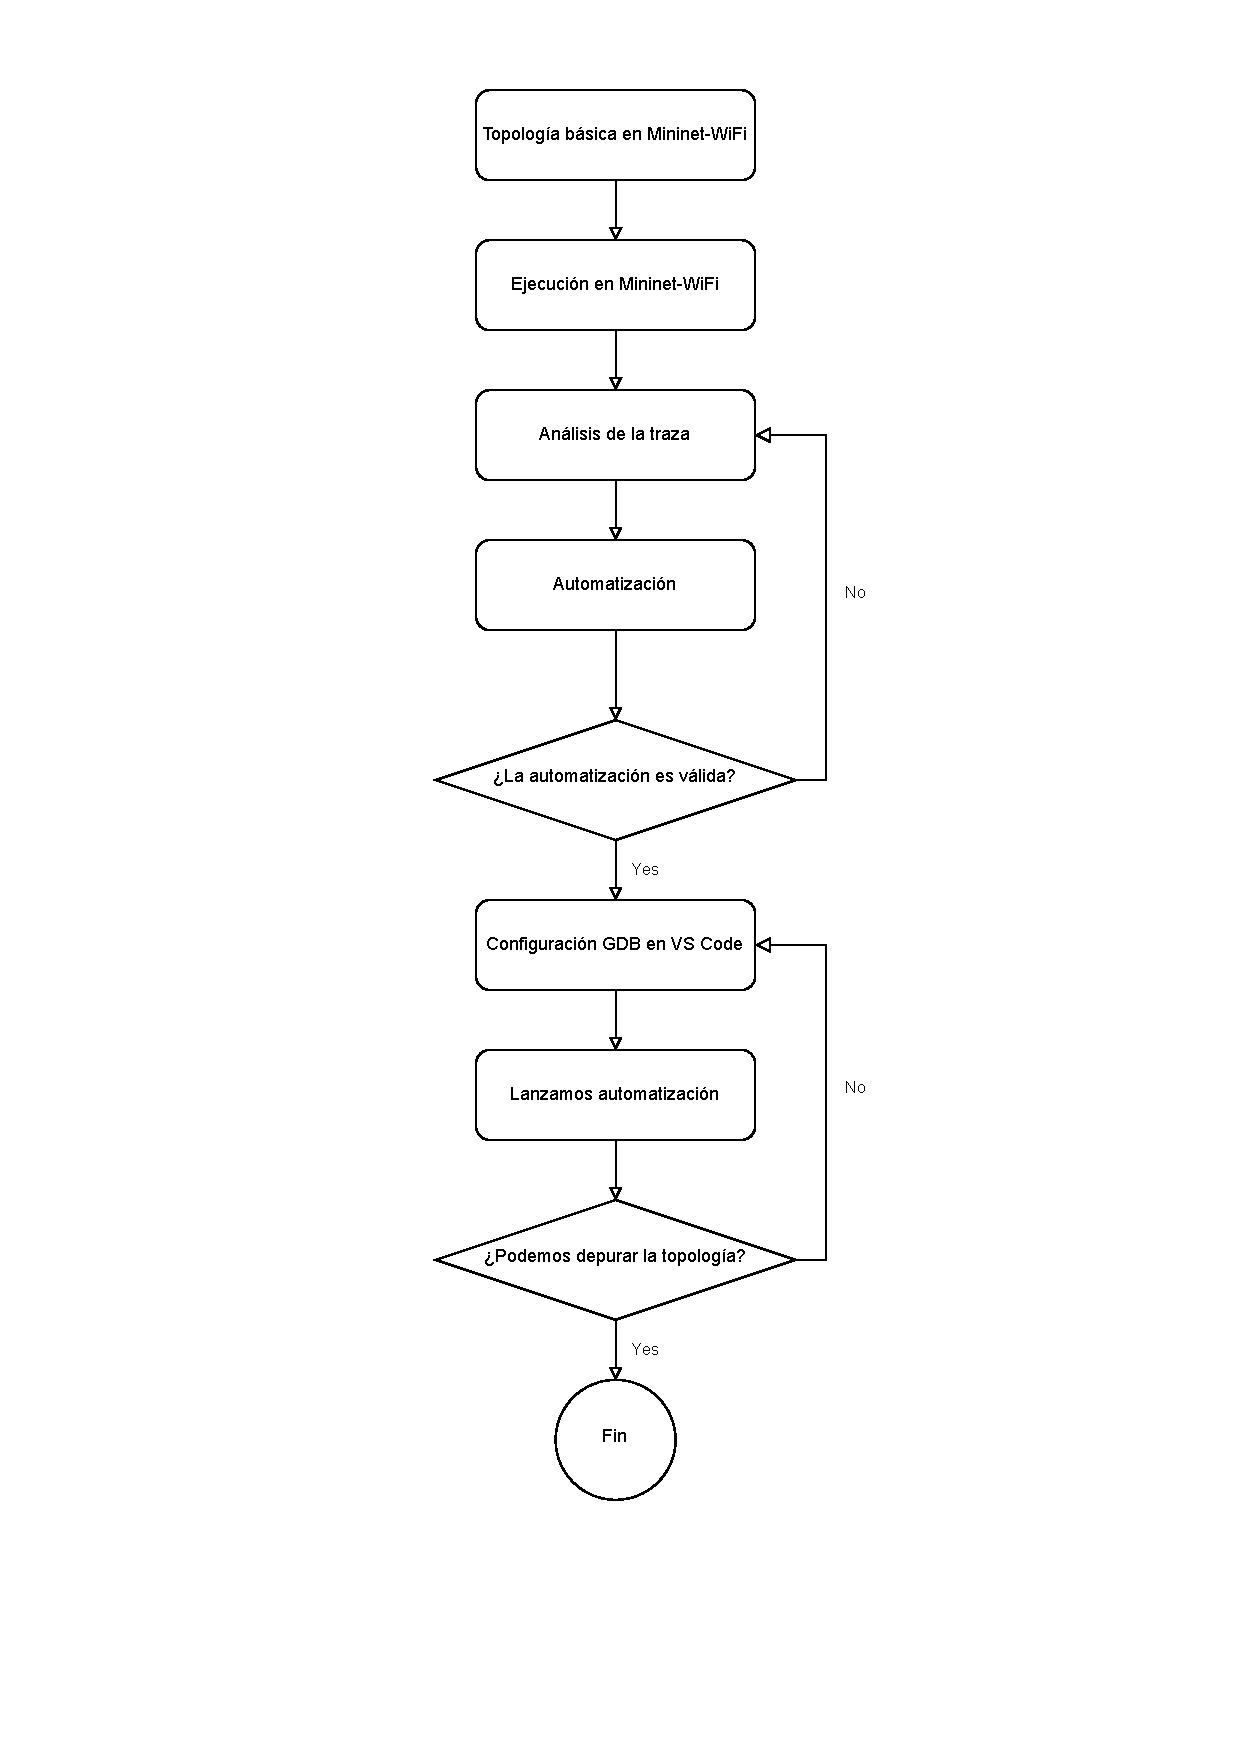
\includegraphics[width=0.9\textwidth]{archivos/img/analisis/debugBOFUSS.drawio.pdf}
    \caption{Proceso de debug al \glsentryshort{bofus}}
    \label{fig:debugBOFUSS}
\end{figure}

\subsection{Limpieza del escenario}

La limpieza del escenario es un proceso muy importante dado que la emulación de todos los escenarios que vayamos lanzando se pueden quedar en nuestro equipo haciendo que se consuman recursos o incluso arrojando un comportamiento no esperado haciendo que las conclusiones sobre los desarrollos bajo test sean incorrectos. Para la limpieza del escenario solo hará falta lanzar el siguiente script que únicamente tiene una línea de código (Ver bloque \ref{code:clean}).\\

\begin{lstlisting}[language= bash, style=Consola, caption={Script de limpieza del escenario - clean.sh},label=code:clean]
    # Lanzamos el script de limpieza del propio Mininet
    sudo mn -c
\end{lstlisting}
\vspace{0.5cm}


La simplicidad del script de limpieza es una de sus principales fortalezas. Aunque pueda parecer básico, este script ha sido probado exhaustivamente en una amplia variedad de configuraciones y topologías, demostrando su eficacia para limpiar de forma completa y agnóstica de la topología todos los componentes relacionados con la interfaz wireless.\\
\\
Durante las pruebas realizadas, en una de ellas, se han ejecutado manualmente los comandos para levantar de forma individual la interfaz wireless para el punto de acceso AP1. En este proceso, se ha observado que el script de limpieza elimina correctamente todas las configuraciones previamente establecidas con nuestro shell script. ¿Cuál es el secreto detrás de esta efectividad?\\
\\
Aquí es donde debemos reconocer el trabajo de Ramon Fontes y su contribución en el desarrollo de Mininet-WiFi. Al examinar el contenido\footnote{\href{https://github.com/intrig-unicamp/mininet-wifi/blob/master/mn_wifi/clean.py\#L77}{mininet-wifi/blob/master/mn\_wifi/clean.py-L77}} de la ruta \texttt{/sys/kernel/debug/ieee80211}, se puede encontrar una lista de todas las interfaces inalámbricas emuladas cargadas en el sistema. Es gracias a esta información que el script de limpieza puede identificar y eliminar de manera precisa todas las configuraciones relacionadas con las interfaces wireless, garantizando una limpieza completa. Como se puede ver en la figura \ref{fig:debugBOFUSS_1}, cuando se lanza el escenario topo.py, al listar las interfaces de la misma forma que lo hace Mininet-WiFi somos capaces de listar todas las interfaces inalámbricas emuladas del sistema, tanto las lanzadas desde Mininet-WiFi como las añadidas a mano haciendo uso de un shell script en paralelo.

\newpage

% fig
\begin{figure}[ht!]
    \centering
    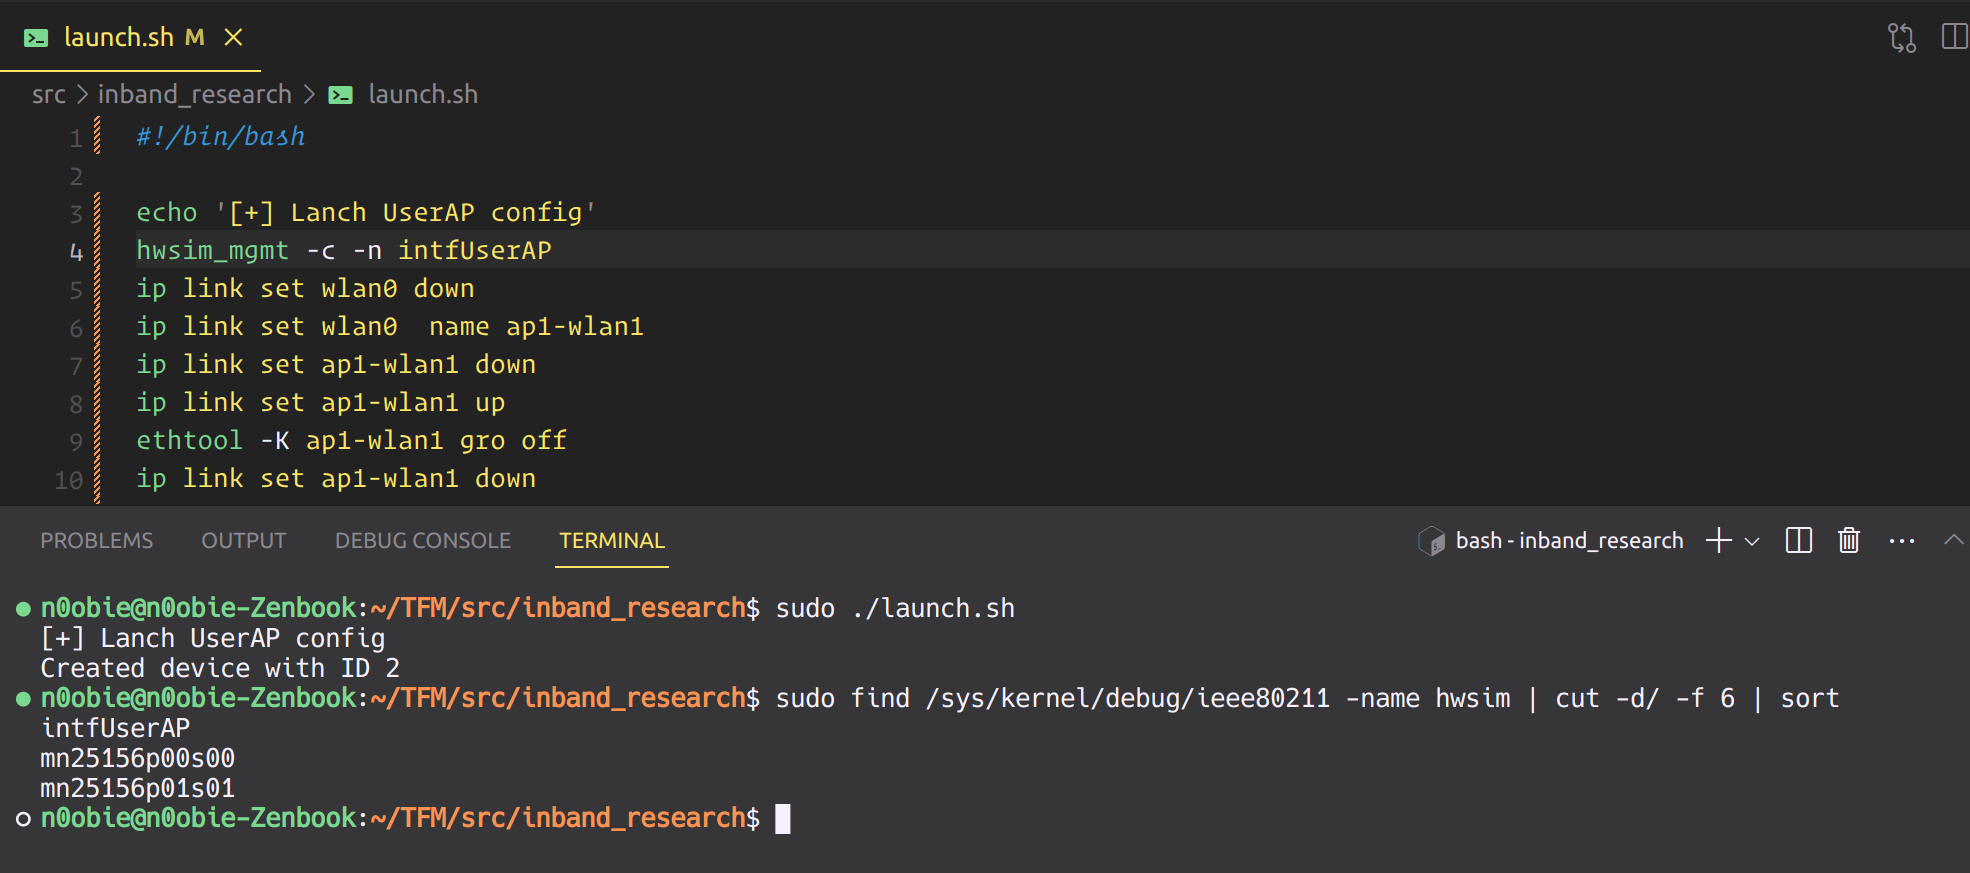
\includegraphics[width=\textwidth]{archivos/img/analisis/debugBOFUSS_1.png}
    \caption{Listado de interfaces inalámbricas en \texttt{/sys/kernel/debug/ieee80211}}
    \label{fig:debugBOFUSS_1}
\end{figure}


Como se puede ver,  como el módulo de limpieza de Mininet-WiFi lee de una ruta desde la cual listan todas las interfaces inalámbricas emuladas, cuando lancemos dicho comando, se listará nuestra capa \textit{phy} emulada, y por ende, será capaz de limpiarla a posteriori.


\subsection{Puesta en marcha del escenario}

Durante el desarrollo del script de puesta en marcha del escenario inalámbrico emulado, se llevó a cabo una exhaustiva investigación para comprender en detalle el funcionamiento interno de la topología básica y la clase \texttt{UserAP} en Mininet-WiFi. Esta investigación fue fundamental para identificar los comandos necesarios y garantizar el correcto funcionamiento del script.\\
\\
Para lograrlo, se analizaron cuidadosamente las trazas de ejecución generadas por el software switch de \texttt{UserAP}. A través de este análisis, se pudo aislar y comprender los comandos utilizados en la creación de radios emuladas. Estas trazas proporcionaron una valiosa información sobre los pasos y procesos involucrados en la configuración de las interfaces inalámbricas. En particular, se observó que la creación de radios emuladas se gestiona mediante la herramienta \texttt{hwsim\_mgmt}. Dentro del código fuente de Mininet-WiFi, este proceso se lleva a cabo en un punto específico y crítico. Este conocimiento fue esencial para extraer los comandos necesarios y adaptarlos al script de lanzamiento del \texttt{UserAP}.\\
\\
El análisis de las trazas y la comprensión del funcionamiento interno de la clase \texttt{UserAP} permitieron obtener una visión clara de los pasos necesarios para configurar y establecer las interfaces inalámbricas emuladas en el escenario. Con esta información en mano, fue posible implementar un script de lanzamiento efectivo que automatiza el proceso y asegura que todas las configuraciones sean aplicadas de manera adecuada (Ver bloque de código \ref{code:launch}).\\

\begin{lstlisting}[language= bash, style=Consola, caption={Script de puesta en marcha del escenario -  launch.sh},label=code:launch]
    #!/bin/bash

    # Vars
    AP_SSID='new-ssid'
    AP_MAC='00:00:00:00:00:01'
    STA_2_CONN=('sta1' 'sta2')

    # Create UserAP
    echo '[+] Lanch UserAP config'
    hwsim_mgmt -c -n intfUserAP
    ip link set wlan0 down
    ip link set wlan0  name ap1-wlan1
    ip link set ap1-wlan1 down 
    ip link set ap1-wlan1 up
    ethtool -K ap1-wlan1 gro off 
    ip link set ap1-wlan1 down 
    ip link set ap1-wlan1 address ${AP_MAC}
    ip link set ap1-wlan1 up
    iw ap1-wlan1 set txpower fixed 100
    echo -e "interface=ap1-wlan1\ndriver=nl80211\nssid=${AP_SSID}\nwds_sta=1\nhw_mode=g\nchannel=1\nctrl_interface=/var/run/hostapd\nctrl_interface_group=0" > mn43736_ap1-wlan1.apconf
    hostapd -B mn43736_ap1-wlan1.apconf
    ip link set ap1-wlan1 down 
    ip link set ap1-wlan1 address ${AP_MAC}
    ip link set ap1-wlan1 up
    tc qdisc replace dev ap1-wlan1 root handle 2: netem rate 54.0000mbit latency 1.00ms
    tc qdisc add dev ap1-wlan1 parent 2:1 handle 10: pfifo limit 1000
    iw dev ap1-wlan1 set txpower fixed 1400
    ofdatapath -i ap1-wlan1 punix:/tmp/ap1 -d 100000000001 --no-slicing 1> /tmp/ap1-ofd.log 2> /tmp/ap1-ofd.log &
    ofprotocol unix:/tmp/ap1 tcp:localhost:6633 --fail=closed  --listen=punix:/tmp/ap1.listen 1> /tmp/ap1-ofp.log 2>/tmp/ap1-ofp.log &

    # Connect stations to AP
    for sta in ${STA_2_CONN[@]}
    do
        echo "[+] Connecting ${sta} to UserAP"
        PID_STA=$(ps aux | grep mininet | grep ${sta} | cut -d' ' -f7)
        echo "[+] ${sta} - Detected pid ${PID_STA}"
        nsenter --target ${PID_STA} --net iwconfig ${sta}-wlan0 essid ${AP_SSID} ap ${AP_MAC}
    done
\end{lstlisting}
\vspace{0.5cm}

Como se puede ver en el bloque de código anterior, primero configuramos lo que viene a ser todos los parámetros propios de la clase \texttt{userAP}, creación de interfaces \textit{wireless} emuladas, configuración de red, además de crear la información requerida con el punto de acceso. Y más adelante lo que se hace es conectar las estaciones WiFi del escenario previamente levantado la red creada por el punto de acceso que se acaba de levantar, accediendo en cada Network namespace de cada estación WiFi.\\
\\
Se quiere añadir un par de detalles que se cree que pueden ser de utilidad al lector en caso de que quieran replicar la depuración \gls{bofus}. Como se ha podido ver para la creación de una radio emulada se tiene que hacer uso del modulo del Kernel mac80211\_hwsim, sin embargo, si se quiere trabajar con el módulo una vez ya insertado en el Kernel tendremos que utilizar otra herramienta. Dicha herrmaienta es \texttt{hwsim\_mgmt}\footnote{\url{https://github.com/patgrosse/mac80211_hwsim_mgmt}}, y a continuación en el bloque de código \ref{code:hwsim} se indican algunos ejemplos de uso de la operativa básica de la herramienta.

\begin{lstlisting}[language= bash, style=Consola, caption={Operativa básica de la herramienta hwsim\_mgmt},label=code:hwsim]
    # Crear una radio emulada
    sudo hwsim_mgmt -c -n [phy_name]

    # Para eliminarlas, se llama a la misma herramienta, de la siguiente manera
    sudo hwsim_mgmt -x [phy_name]
\end{lstlisting}
\vspace{0.5cm}

Es necesario que para trabajar con la herramienta, \texttt{hwsim\_mgmt}, que el modulo del kernel mac80211\_hwsim esté cargado, si no lo está, no podremos crear ninguna radio nueva. En la figura \ref{fig:debugBOFUSS_2} se ilustra como podemos comprobar si el módulo está previamente cargado. En este caso, si vamos a lanzar primero el script de la topología básica en primera instancia \texttt{topo.py},  el cual ya cargará el modulo, no será necesario tener que cargarlo. Si creamos una interfaz con el modulo ya cargado podemos comprobar que se ha creado un nuevo radio de la siguiente forma (Ver figura \ref{fig:debugBOFUSS_3}).

% fig
\begin{figure}[ht!]
    \centering
    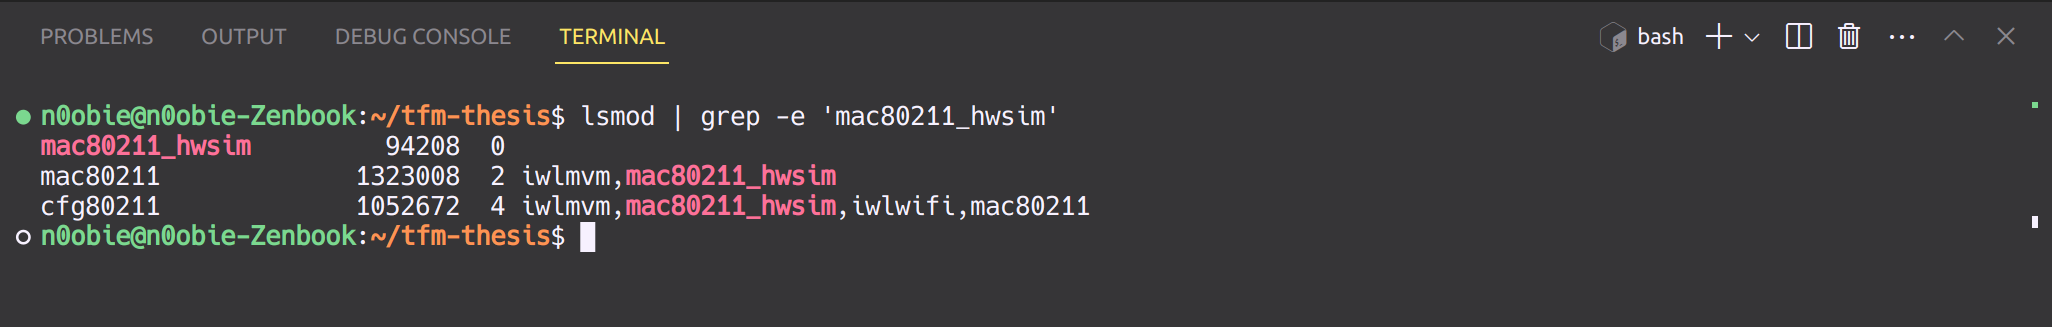
\includegraphics[width=\textwidth]{archivos/img/analisis/debugBOFUSS_2.png}
    \caption{Comprobación de si el módulo \texttt{mac80211\_hwsim} está cargado}
    \label{fig:debugBOFUSS_2}
\end{figure}

% fig
\begin{figure}[ht!]
    \centering
    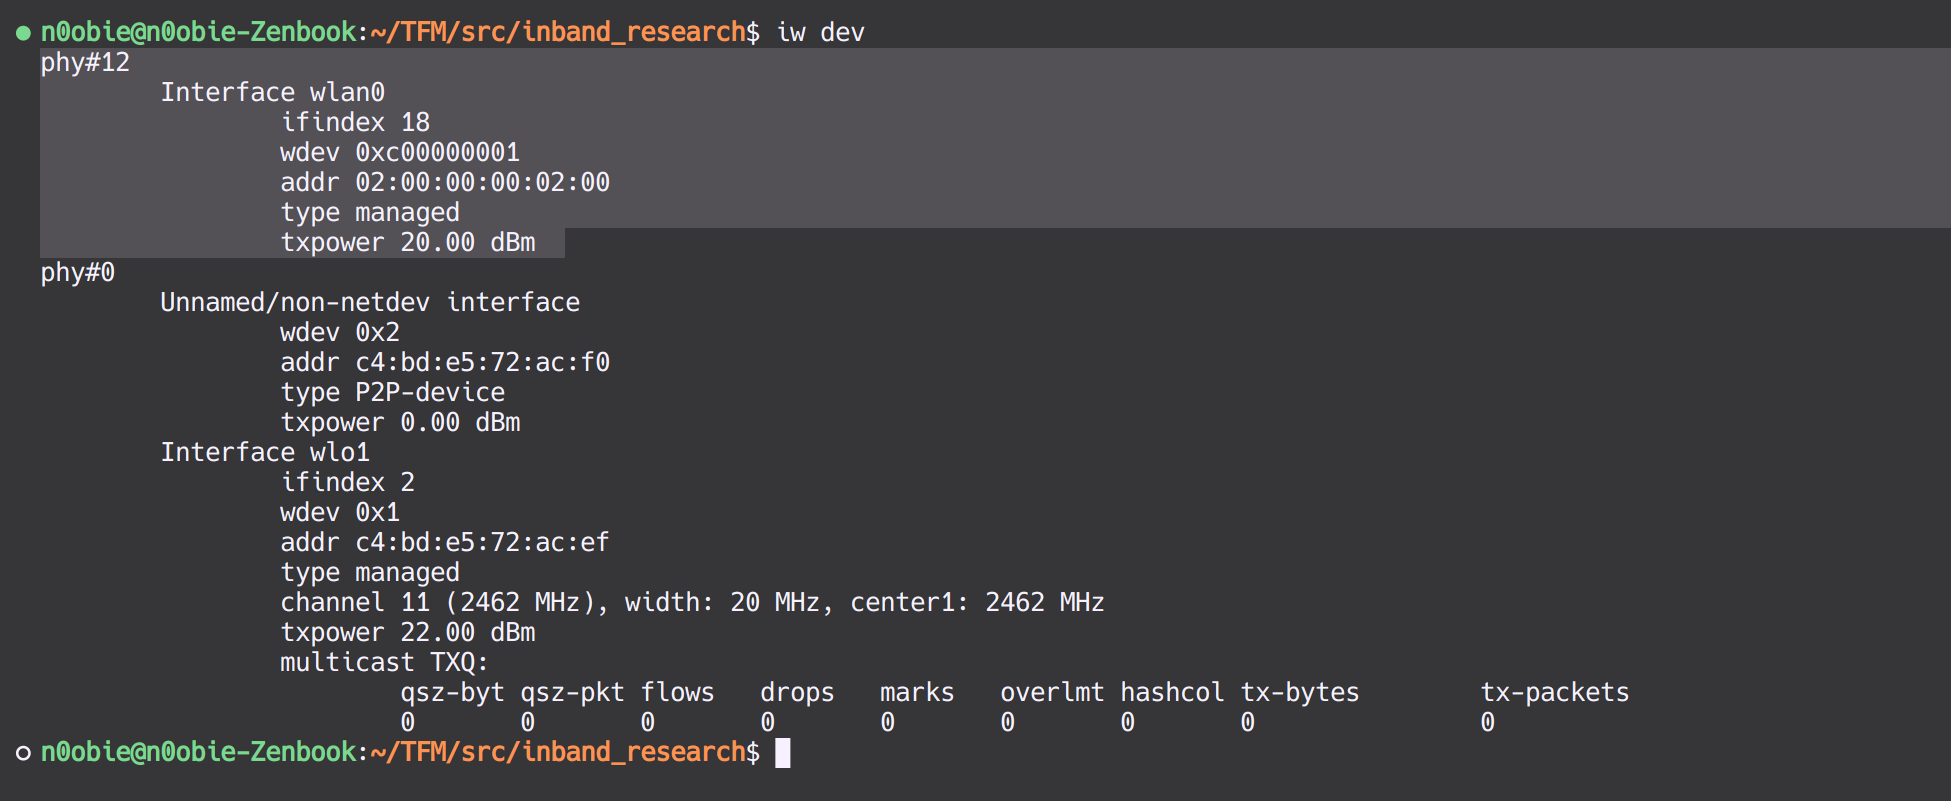
\includegraphics[width=\textwidth]{archivos/img/analisis/debugBOFUSS_3.png}
    \caption{Listado de \textit{phy} inalámbricas usando el comando \texttt{iw}}
    \label{fig:debugBOFUSS_3}
\end{figure}


\subsubsection{Troubleshooting}

Uno de los problemas más comunes que pueden surgir durante el desarrollo del escenario inalámbrico emulado, es que en algunas ocasiones, nos podemos encontrar con que la interfaz inalámbrica se bloquea y nos muestra un mensaje de advertencia indicando lo siguiente:

\begin{lstlisting}[language= bash, style=Consola, caption={Bloqueo de la interfaz por RF-Kill},label=code:rfkills1]
    ~$  Operation not possible due to RF-kill
\end{lstlisting}
\vspace{0.5cm}

Este mensaje indica que la interfaz inalámbrica está bloqueada por una restricción llamada  ``RF-kill". Esta restricción puede ser causada por diferentes factores, como un interrupción mal gestionada, una mala configuración del sistema operativo, o para salvaguardar los recursos de la máquina. Pero generalmente son \textit{soft-blocked} por el Kernel, en la mayoria de los casos para auto-protegerse. Para solucionar este problema, debemos ejecutar el siguiente comando en la terminal (Ver bloque de código \ref{code:rfkills2}).\\

\begin{lstlisting}[language= bash, style=Consola, caption={desbloqueo de la interfaz por RF-Kill},label=code:rfkills2]
    rfkill unblock all
\end{lstlisting}
\vspace{0.5cm}

Este comando desbloqueará todas las interfaces inalámbricas que estén afectadas por la restricción "RF-kill". Una vez ejecutado el comando, la interfaz inalámbrica estará disponible y podremos establecerla en el estado \texttt{UP} sin problemas.  Si el problema persiste después de ejecutar el comando mencionado, es recomendable verificar otros posibles problemas, como configuraciones incorrectas o conflictos en el sistema.

\subsection{Configuración de VS Code}

Para configurar Visual Studio Code  y poder depurar el \gls{bofus} utilizando GDB, crearemos un archivo JSON con la configuración necesaria. Antes de eso, es importante destacar que hemos logrado lanzar un escenario y ejecutar un UserAP desde un script de shell. Ahora debemos crear un archivo JSON en VS Code que invoque las dos últimas líneas de ofdatapath y ofprotocol para depurar los binarios. Por lo tanto, debemos parametrizar las instrucciones (Líneas del bloque de código \ref{code:bofussLaunch}) en el JSON de depuración. A continuación, en el bloque \ref{code:gdbjson}, se indica el JSON de configuración para la depuración.

\begin{lstlisting}[language= bash, style=Consola, caption={JSON de depuración con GDB del BOFUSS},label=code:gdbjson]
    {
        "version": "0.2.0",
        "configurations": [
            {
                "name": "(ap1)ofprotocol",
                "type": "cppdbg",
                "request": "launch",
                "program": "${workspaceFolder}/secchan/ofprotocol",
                "args": [
                    "unix:/tmp/ap1",
                    "tcp:localhost:6653",
                    "--fail=closed",
                    "--listen=punix:/tmp/ap1.listen"
                ],
                "stopAtEntry": false,
                "cwd": "${workspaceFolder}",
                "environment": [],
                "externalConsole": false,
                "MIMode": "gdb",
                "setupCommands": [
                    {
                        "text": "target-run",
                        "description": "Ofprotocol",
                        "ignoreFailures": true
                    }
                ]
            },
            {
                "name": "(ap1)ofdatapath",
                "type": "cppdbg",
                "request": "launch",
                "program": "${workspaceFolder}/udatapath/ofdatapath",
                "args": [
                    "-i",
                    "ap1-wlan1",
                    "punix:/tmp/ap1",
                    "-d",
                    "000000000001",
                    "--no-slicing"
                ],
                "stopAtEntry": false,
                "cwd": "${workspaceFolder}",
                "environment": [],
                "externalConsole": false,
                "MIMode": "gdb",
                "setupCommands": [
                    {
                        "text": "target-run",
                        "description": "Ofdatapath",
                        "ignoreFailures": true
                    }
                ]
            }
        ],
        "compounds": [
            {
                "name": "(ap1)ofprotocol/(ap1)ofdatapath",
                "configurations": [
                    "(ap1)ofprotocol",
                    "(ap1)ofdatapath"
                ],
                "preLaunchTask": "${defaultBuildTask}",
                "stopAll": true
            }
        ]
    }
\end{lstlisting}
\vspace{0.5cm}


Es importante mencionar que GDB no admite la ejecución con privilegios de root directamente. Para solucionar este problema, es necesario realizar un ajuste adicional\footnote{\url{https://github.com/microsoft/vscode-cmake-tools/issues/2463}}\footnote{\url{https://github.com/microsoft/vscode-cpptools/issues/861}}.

%%%%%%%%%%%%%%%%%%%%%%%%%%%%%%%%%%%%%%%%%%%%%%%%%%%%%%%%%%%%%%%%%%%%%%%%%%%%%%%%%%%%%%%%%%%%%%%%%

%\chapter{Desarrollo y evaluación del protocolo}
\label{desarrollo}

% intro
En este capítulo, se abordará el desarrollo del protocolo en la plataforma seleccionada, destacando las partes más relevantes del proceso. Además, se realizará una evaluación exhaustiva para analizar su funcionamiento de manera funcional y cuantitativa. El objetivo principal de este capítulo es presentar el resultado del desarrollo realizado, mostrando cómo se ha implementado el protocolo en el entorno seleccionado para el proyecto. Se destacarán aquellas etapas del desarrollo que se consideran de mayor importancia debido a su impacto en el rendimiento y la efectividad del protocolo.\\
\\
Se comenzará describiendo detalladamente la arquitectura y los componentes del protocolo, explicando su funcionamiento en el contexto de la plataforma elegida. Se hará especial hincapié en los aspectos clave que diferencian al protocolo y que lo hacen una solución innovadora en el ámbito del control in-band para entornos de IoT. A continuación, se presentará el proceso de implementación, resaltando los desafíos y decisiones clave que se han enfrentado durante el desarrollo. Se discutirán las técnicas y algoritmos utilizados para lograr la funcionalidad deseada, asegurando una comprensión clara de la implementación realizada. Posteriormente, se llevará a cabo una evaluación detallada del protocolo desarrollado. Esta evaluación permitirá obtener una visión clara y objetiva del rendimiento del protocolo, proporcionando una base sólida para la toma de decisiones y posibles mejoras futuras. Se presentarán los resultados obtenidos y se discutirán las implicaciones y conclusiones derivadas de ellos.

%%%%%%%%%%%%%%%%%%%%%%%%%%%%%%%%%%%%%%%%%%%%%%%%%%%%%%%%%%%%%
\section{Entorno de desarrollo y validación}
\label{sec:scenarioDEV}


%%%%%%%%%%%%%%%%%%%%%%%%%%%%%%%%%%%%%%%%%%%%%%%%%%%%%%%%%%%%%
\section{Desarrollo interfaz de control del Datapath - \texttt{dpctl}}
\label{sec:dpctl}

En esta sección se va a estudiar el funcionamiento interno de la herramienta \texttt{dpctl}\footnote{\url{https://github.com/CPqD/ofsoftswitch13/blob/master/utilities/dpctl.c}} la cual se utiliza para gestionar y controlar el plano de datos de software switch BOFUSS. La motivación de esta sección radica en el desarrollo realizado para adaptar su funcionamiento a raíz de encontrar serios problemas en su interfaz de comandos. Dichos problemas e incompatibilidades llevan registrados en varios \textit{issues}\footnote{\url{https://github.com/mininet/mininet/issues/745}}\footnote{\url{https://github.com/CPqD/ofsoftswitch13/issues/288}}\footnote{\url{https://github.com/mininet/mininet/issues/628}} desde el 2018 tanto en Mininet como en el repositorio de \gls{bofus}, lo que hacía ingestionable la comprobación del correcto funcionamiento del software switch modificado.

%%%%%%%%%%%%%%%%%%%%%%%%%%%%%%%%%%%%%%%%%%%%%%%%%%%%%%%%%%%%%
\section{Implementación del protocolo IoTorii}
\label{sec:devIOTTORIII}

En esta sección se va a explicar la implementación realizada del protocolo IoTorii en el \textit{software switch} \gls{bofus}. Dado que el trabajo de implementación ha sido bastante extenso, dado que había que discernir que parte de la implementación del control in-band podía ser aprovechada, se ha decidido generar un documento anexo \cite{davidBOFUSS} aparte de la memoria, donde se explique a bajo nivel las modificaciones realizadas. Todo el código se puede encontrar indicado en la Sección \ref{sec:estadoArte_github}. \\
\\
En la Figura \ref{fig:WIN-BOFUSS}, se puede apreciar la secuencia lógica que se ha llevado a cabo para la implementación del protocolo IoTorii en el software switch. En adelante se podrá encontrar el termino \texttt{win-BOFUSS}, el cual hará referencia a la implementación del protocolo IoTorii en la implementación de in-band del \gls{bofus}, conocida como \texttt{in-BOFUSS}, por lo que para añadirle la condición de \textit{wireless} se ha apodado como \texttt{win-BOFUSS}, del inglés \textit{\textbf{w}ireless \textbf{in}-band \textbf{B}asic \textbf{O}pen\textbf{F}low \textbf{U}serspace \textbf{S}oftware \textbf{S}witch}.\\

% fig
\begin{figure}[ht!]
    \centering
    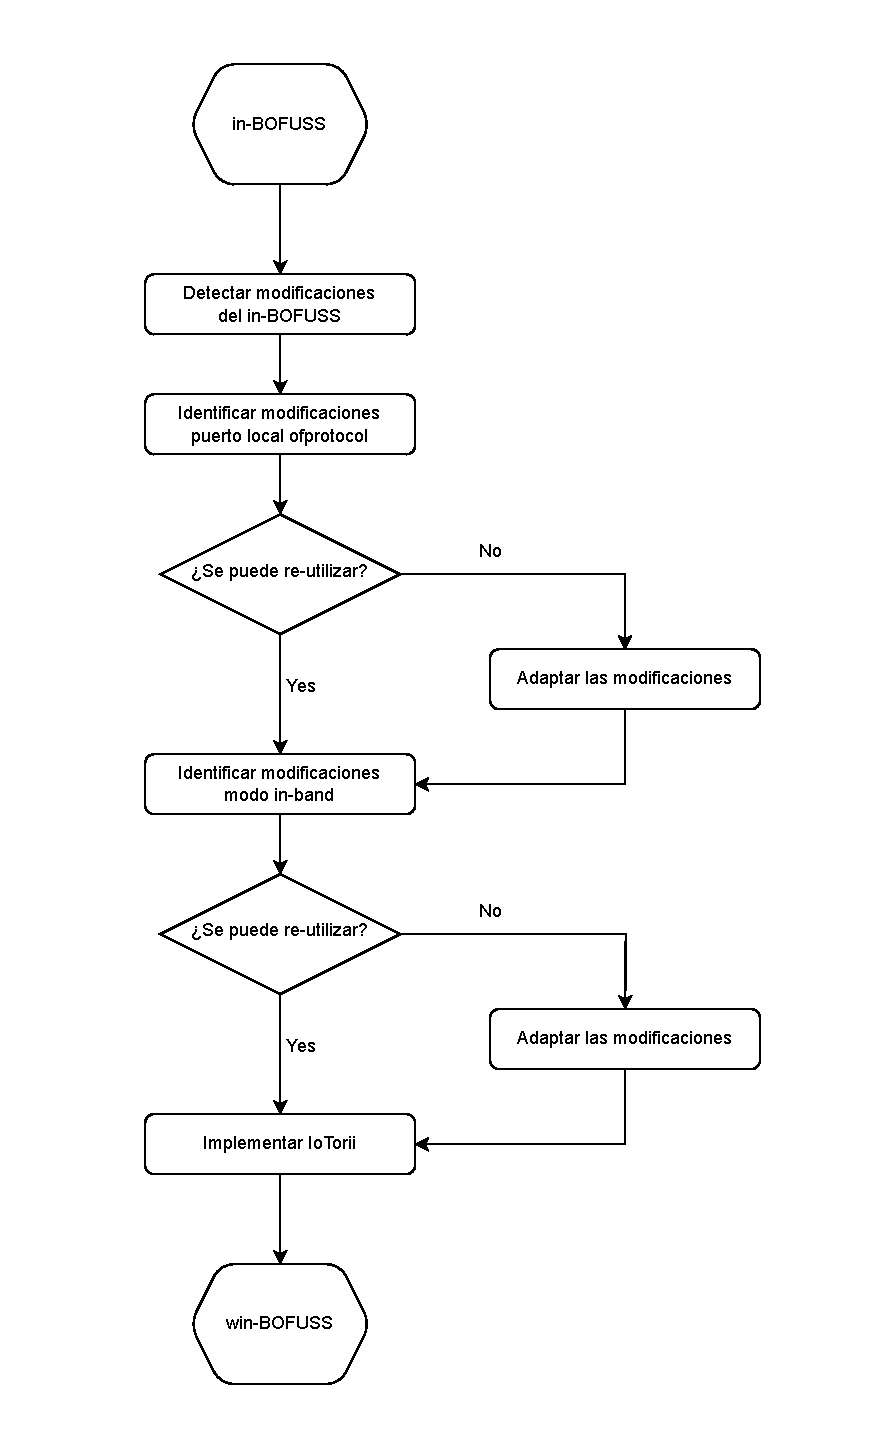
\includegraphics[width=0.75\textwidth]{archivos/img/dev/winBOFUSS.pdf}
    \caption{Diagrama de flujo para la implementación del protocolo IoTorii en el software switch \glsentryshort{bofus}}
    \label{fig:WIN-BOFUSS}
\end{figure}

La implementación de IoTorii está basada en una publicación del grupo de investigación NetIS de la Universidad de Alcalá \cite{rojas2021outperforming}. El funcionamiento del protocolo está descrito en la Sección \ref{sec:ana_inband}, y con él conseguiremos crear múltiples caminos desde cualquier nodo de la topología al nodo raíz. La idea de utilizar este protocolo según se comentó es para tener caminos de respaldo en cada nodo hacia el nodo raíz, pudiendo conmutar de uno a otro cuando sea necesario, bien sea porque un equipo ha fallado o porque al ser un entorno inalámbrico donde la movilidad es intrinseca el \textit{next-hop} al nodo raíz ya no se encuentra en rango.\\
\\
En la Figura \ref{fig:iotoriiFulls}, se indica el diagrama de flujo con la implementación del protocolo en el \gls{bofus}. En primer lugar, al poner el switch en el modo de control in-band, se inicializa la lógica de IoTorii. Una vez que el protocolo IoTorii ha sido inicializado, el nodo raíz comienza la exploración, propagando los paquetes utilizados para generar los caminos que posteriormente serán almacenados en las tablas IoTorii de los nodos. Dichos paquetes, de tipo \textit{SetHLMAC}, solo serán entregados a los nodos que cumplan la condición de vecinos, es decir, aquellos nodos que hayan sido notificados mediante un mensaje de tipo \textit{Hello}. Cuando una ruta de la tabla HLMAC no se ve renovada, es decir, el nodo anexo al siguiente salto de esa ruta no ha enviado un mensaje de tipo \textit{Hello}, esta ruta se invalidará y se saltará a la siguiente dentro de la tabla HLMAC. Cuando esto ocurre el puerto local será el mismo, dado que la interfaz será la misma, pero el \textit{next-hop} no lo será dado que cambiará, habrá que actulizar la MAC destino en la conexión TCP que se realiza através de un mensaje netlink al stack de red del Kernel. \\
\\
En un entorno Linux, es posible utilizar Netlink para modificar la dirección MAC de destino asociada a una IP específica en la tabla ARP. Netlink es una interfaz de comunicación entre el espacio de usuario y el espacio de Kernel que permite realizar diversas operaciones relacionadas con la configuración de red. Lo primero que se tiene que llevar a cado en esta operación es abrir una conexión Netlink para comunicarse con el Kernel. Esto implica crear un socket Netlink y enlazarlo a un tipo de mensaje Netlink en específico. Acto seguido, se tiene que preparar el mensaje Netlink de tipo \texttt{RTM\_NEWNEIGH} (mensaje utilizado para manipular la caché ARP), y establecer los atributos del mensaje, configurando los atributos del mensaje para indicar la IP y la nueva dirección MAC destino a fijar. Enviar dicho mensaje y gestionar la confirmación del Kernel. De esta forma podremos actualizar de una ruta HLMAC a otra, pero lamentablemente no se ha conseguido hacer la operación de forma automática sin cerrar el socket por lo que será necesario volver a abrir el socket TCP con el controlador.\\
\\



\begin{figure}[ht!]
    \centering
    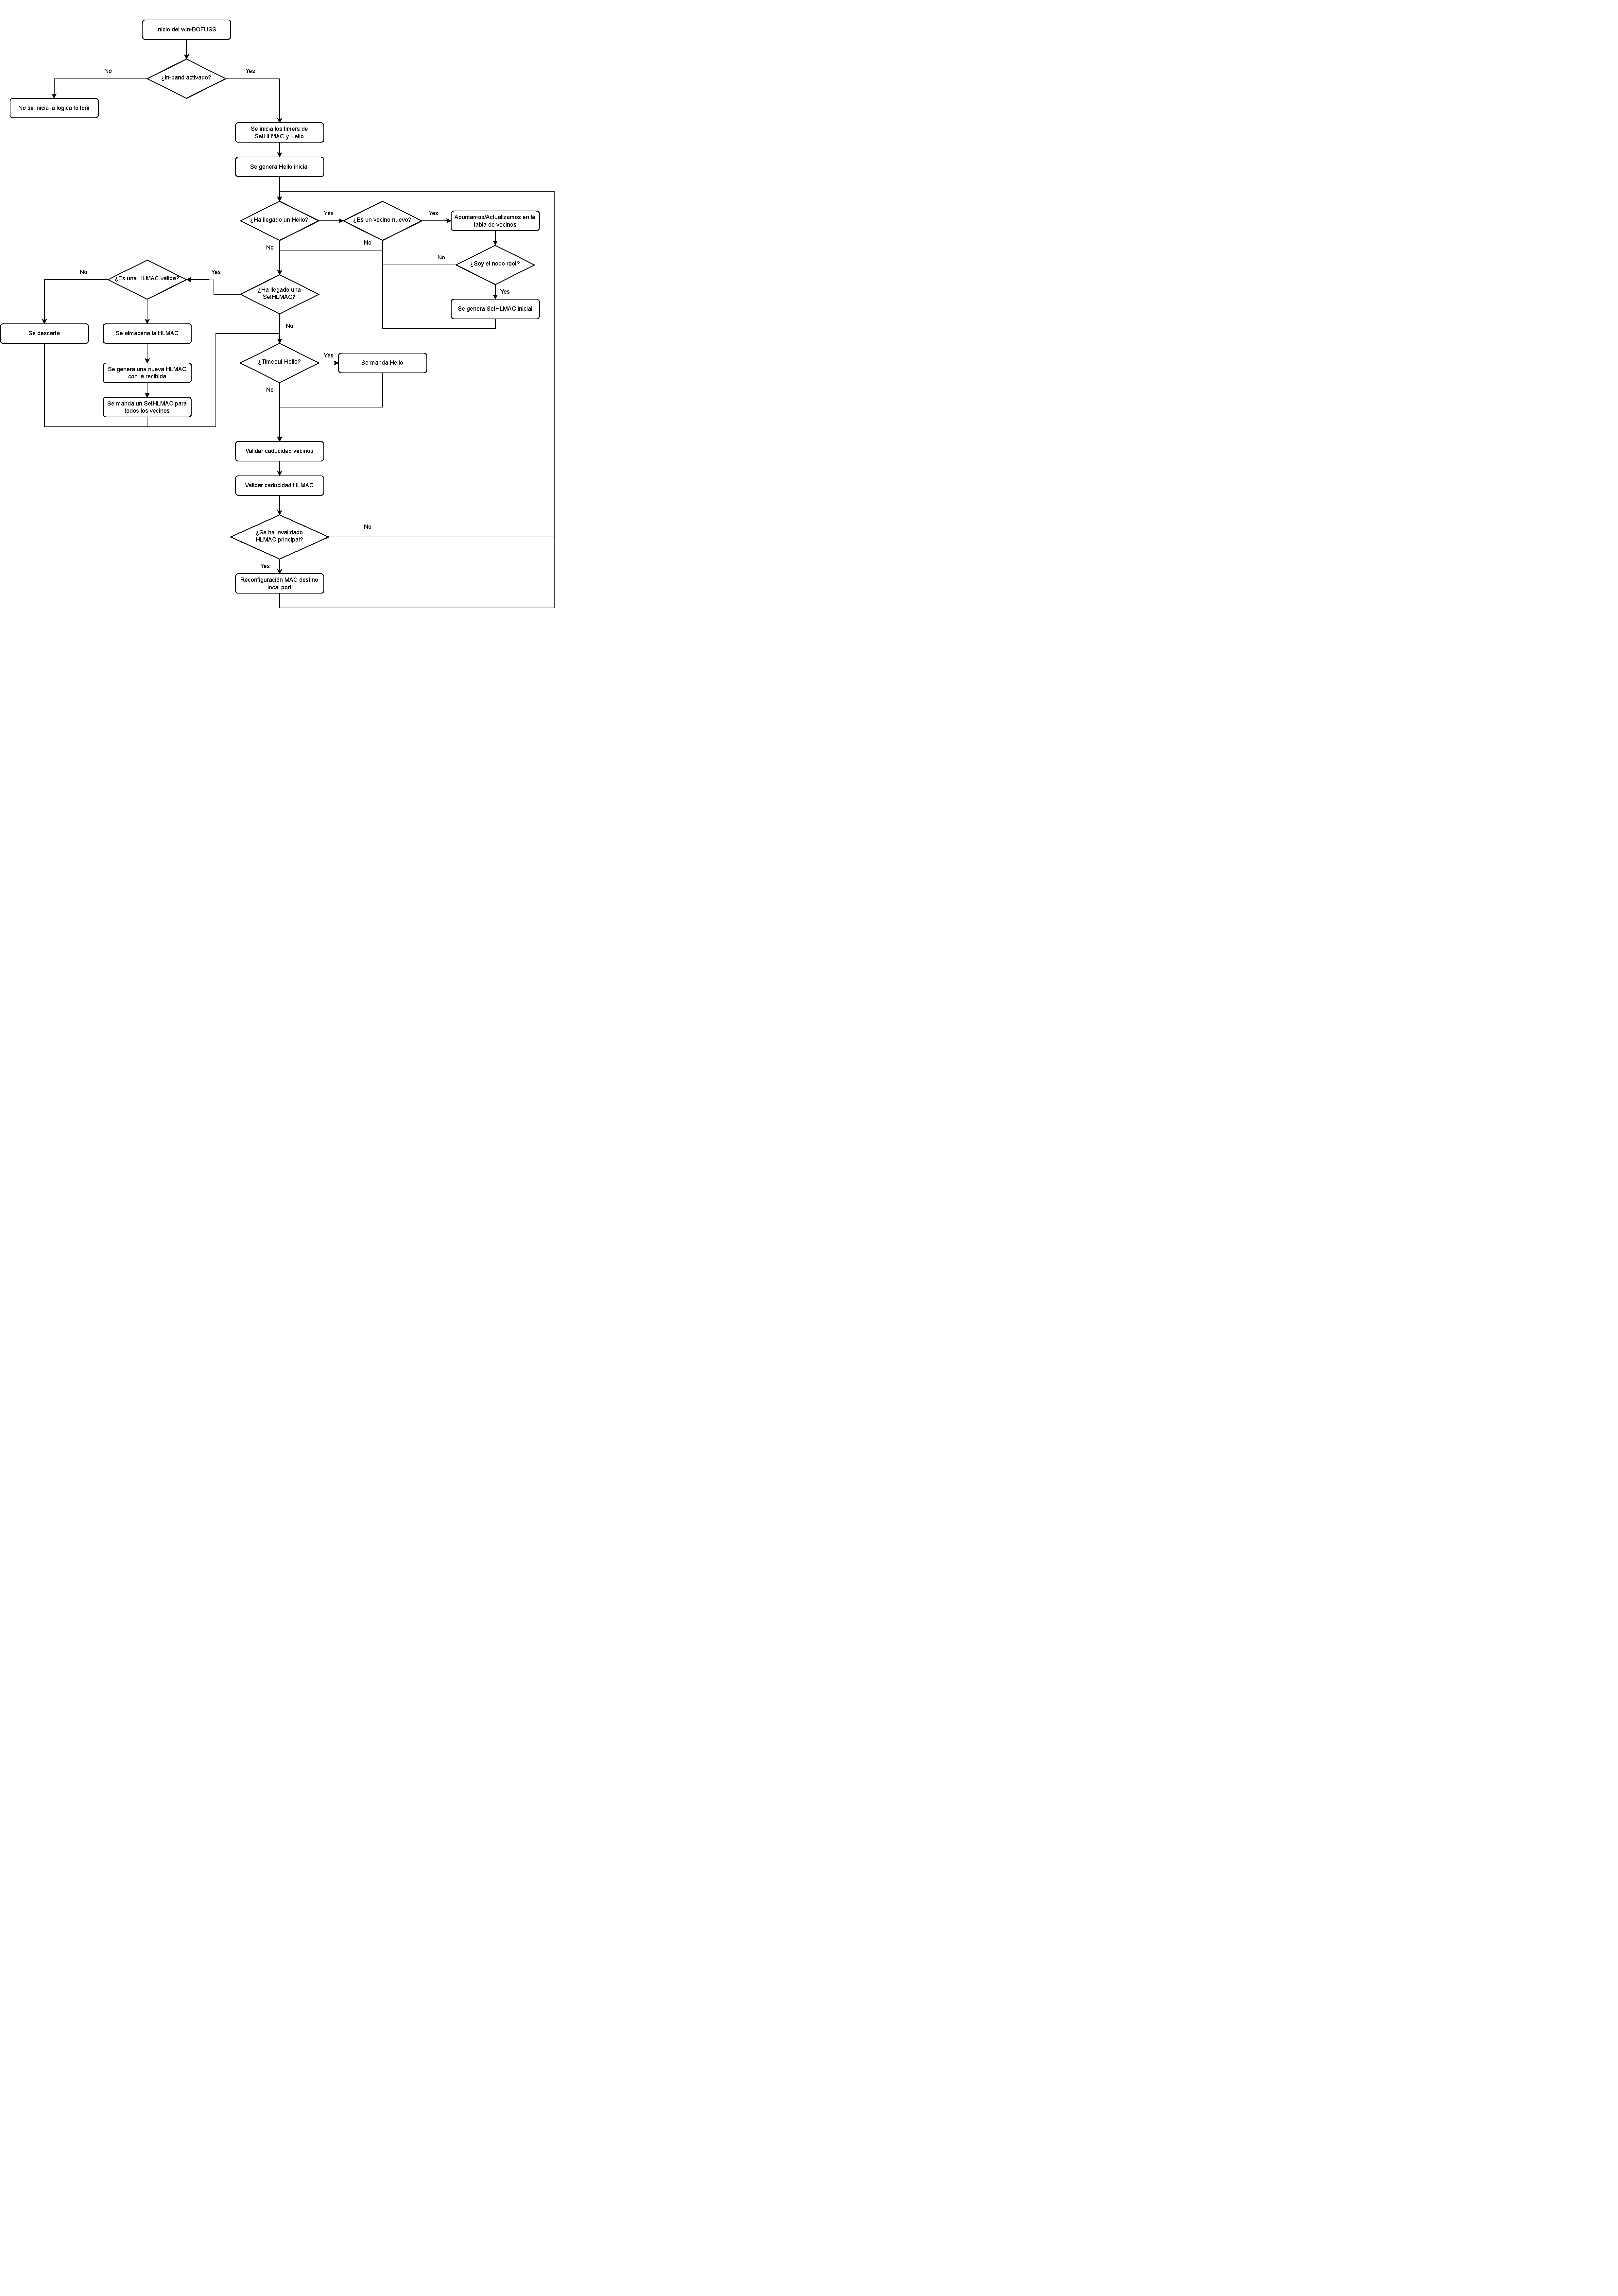
\includegraphics[width=\textwidth]{archivos/img/dev/iotorii.pdf}
    \caption{Diagrama de flujo de la operativa del protocolo IoTorii en el software switch \glsentryshort{bofus}}
    \label{fig:iotoriiFulls}
\end{figure}

\newpage

La importancia de establecer un temporizador para los mensajes \textit{Hello} y definir la caducidad de los vecinos en un protocolo radica en la mejora de su resiliencia y capacidad para adaptarse a cambios en la topología de la red. Estos mecanismos son fundamentales para mantener la conectividad y la estabilidad del protocolo en entornos dinámicos.\\
\\
El temporizador de los mensajes \textit{Hello} determina la frecuencia con la que los nodos del protocolo intercambian información de vecindad. Estos mensajes \textit{Hello} son vitales para conocer y mantener actualizada la lista de vecinos en la red. Al establecer un temporizador adecuado, se asegura que los nodos compartan regularmente información sobre su disponibilidad, estado y conexiones. Esto permite identificar rápidamente cambios en la topología de la red, como la caída de un enlace o la aparición de nuevos nodos. La caducidad de los vecinos define el tiempo que un nodo considera que un vecino sigue siendo alcanzable y activo. Cuando un vecino no responde a los mensajes \textit{Hello} dentro de este período, se considera que ha caducado y se elimina de la lista de vecinos. Establecer una caducidad adecuada es esencial para detectar y reaccionar rápidamente ante la pérdida de conectividad con un vecino. Al eliminar los vecinos caducados, se evita enviar tráfico a nodos inalcanzables y se garantiza que los recursos de red se utilicen de manera eficiente.\\
\\
La resilencia de un protocolo depende en gran medida de su capacidad para recuperarse rápidamente de fallos en la red y adaptarse a cambios en la topología. Al establecer un temporizador de mensajes \textit{Hello} y una caducidad de vecinos adecuados, el protocolo puede detectar y responder de manera oportuna a eventos como enlaces caídos, nodos inalcanzables o nuevos vecinos. Esto permite que el protocolo reconstruya rápidamente su tabla de vecinos y ajuste sus rutas en consecuencia, minimizando el impacto de las fallos y optimizando la utilización de los recursos de red.\\
\\
A continuación, se van a indicar algunas de las modificaciones más importantes a la hora de implementar la lógica del protocolo IoTorii:

\begin{itemize}
    \item La estructura \texttt{reg\_HLMAC}, ha sido creada para representar una entrada de la tabla de HLMACs, también conocida como tabla de rutas de IoTorii. Cada entrada tiene almacenada la HLMAC, un flag de si está activa o no.
    \item La estructura \texttt{table\_HLMAC}, ha sido creada para representar la tabla de HLMACs, que viene a ser una lista enlazada simple de estructuras \texttt{reg\_HLMAC}.
    \item La estructura \texttt{reg\_nb}, ha sido creada para representar una entrada de la tabla de vecinos. Cada entrada tiene almacenada la MAC real del vecino, un flag de si está activa o no, y el sufijo único asignado.
    \item La estructura \texttt{table\_nb}, ha sido creada para representar la tabla de vecinos, que viene a ser también una lista enlazada simple de estructuras \texttt{reg\_nb}.
    \item Se ha adaptado la función \texttt{table\_AMACS\_add\_AMAC()} con las nuevas estructuras de datos, para que gestione el guardado de las HLMACs de IoTorii en vez de las AMACs. La función se ha renombrado a \texttt{table\_HLMACS\_add\_HLMAC()}.
    \item Se ha modificado la función \texttt{dp\_ports\_output\_amaru()}, la cual se encargaba de crear y enviar un paquete de Amaru por todas las interfaces del switch, para que ahora, dado que solo va a haber una interfaz genere los mensajes \textit{SetHLMAC} por la interfaz por los $N$ vecinos que tenga el nodo en cuestión. La función se ha renombrado a \texttt{dp\_ports\_output\_iotorii()}.
    \item Se han adaptado las funciones \texttt{disable\_invalid\_amacs\_UAH()} y \texttt{enable\_valid\_\\amacs\_UAH()}, las cuales se utilizaban para conmutar el \textit{flag} de active de las rutas, para que puedan trabajar con las nuevas estructuras de datos HLMAC. Las funciones se han renombrado a \texttt{disable\_invalid\_hlmacs\_UAH()} y \texttt{enable\_valid\_hlmacs\_UAH()} respectivamente.
    \item Se ha modificado la función \texttt{configure\_new\_local\_port\_amaru\_UAH()}, la cual se encargaba de buscar en la tabla de rutas AMACS, para que busque en la nueva tabla HLMAC y que aparte gestione el traspaso de una ruta a otra, modificando vía Netlink la nueva MAC destino del siguiente salto. La función se ha renombrado a \texttt{configure\_new\_local\_port\_iotorii\_UAH()}.
    \item Se ha modificado la función \texttt{send\_amaru\_new\_localport\_packet\_UAH()}, para que ajuste las reglas de las tablas de flujos del ofdatapath mediante una generación de un mensaje de tipo \texttt{PACKET\_IN} que se envía al ofprotocol.
    \item Se ha modificado la función \texttt{dp\_ports\_run()}, la cual de forma periorida verificará el estado del puerto, y además gestionará las funciones \texttt{disable\_invalid\_amacs\_UAH()} y \texttt{enable\_valid\_amacs\_UAH()} verificando la caducidad de las entradas. En caso de caducar una ruta activa se llamará a la función, \texttt{install\_new\_localport\_rules\_UAH()}, y a la función \texttt{configure\_new\_local\_port\_iotorii\_UAH()} para gestionar la instalación de una ruta alternativa.
    \item Se han creado una lógica de control de timer para la generación de los mensajes \textit{Hello}s. Toda la lógica está incluida en la función \texttt{timer\_UAH()}.
\end{itemize}

\subsection{Despliegue de la implementación en una RPi}

Durante el proceso de desarrollo, se ha realizado un intento exhaustivo para desplegar la implementación completa del protocolo IoTorii en una Raspberry Pi (RPi). Sin embargo, hasta el momento, este intento no ha alcanzado el éxito debido a una problemática relacionada con la traducción de símbolos que se realiza en la librería de \texttt{oflib}. Se ha identificado que esta traducción debe ser corregida para lograr un despliegue funcional en dicha plataforma, pero se escapa de los objetivos del \gls{tfm}. Por otro lado, se ha observado que el despliegue del \gls{bofus}, una vez se ha corregido el funcionamiento interno de la librería en cuestión, debería ser inmediato, ya que el entorno Linux es el mismo, y solo se requiere adaptarse correctamente a la arquitectura. Es relevante mencionar que se ha identificado un \textit{issue} específico que refleja esta misma problemática de despliegue sobre una arquitectura ARM, la misma que se ha visto a la hora de desplegar la implementación del protocolo IoTorii.

\begin{itemize}
    \item Dicho \textit{issue}  puede consultarse en el siguiente enlace: \url{https://github.com/CPqD/ofsoftswitch13/issues/196}
\end{itemize}



%%%%%%%%%%%%%%%%%%%%%%%%%%%%%%%%%%%%%%%%%%%%%%%%%%%%%%%%%%%%%
\section{Validación}
\label{sec:vali}

En esta sección, se presenta una descripción exhaustiva de los escenarios y pruebas llevadas a cabo para verificar el correcto funcionamiento de las implementaciones realizadas. El propósito de estas pruebas es validar el correcto desempeño de las modificaciones implementadas, tal como se detalla en la sección previa.

Cabe destacar que las pruebas desarrolladas en este capítulo no tienen como objetivo cuantificar el rendimiento del switch BOFUSS por diversas razones. En primer lugar, dicho enfoque no ha sido establecido como objetivo principal del presente TFM (Trabajo de Fin de Máster). En segundo lugar, el switch BOFUSS se encuentra más orientado hacia el prototipado y desarrollo de nuevas funcionalidades que a lograr un rendimiento excepcional en el procesamiento de los paquetes.

En consecuencia, el enfoque de las pruebas se centra en verificar el funcionamiento adecuado de las implementaciones realizadas, sin ahondar en la medición precisa del rendimiento del switch BOFUSS.

\subsection{Comprobación funcional}

% Lets see tomorrow
%\subsection{Comprobación cuantitativa}


%%%%%%%%%%%%%%%%%%%%%%%%%%%%%%%%%%%%%%%%%%%%%%%%%%%%%%%%%%%%%
%\chapter{Conclusiones y trabajo futuro}
\label{conclusiones}

En este capítulo, se concluirá la memoria presentando las conclusiones del trabajo realizado y evaluando tanto el trabajo en sí como los resultados obtenidos durante el desarrollo. Además, se explorarán las posibles vías de trabajo futuro que surgieron a medida que se llevaba a cabo el TFM. Se presentarán estas vías y se cerrará la memoria con una visión general y reflexiva sobre el proyecto realizado.


%%%%%%%%%%%%%%%%%%%%%%%%%%%%%%%%%%%%%%%%%%%%%%%%%%%%%%%%%%%%%%%%%%%%%%%%%%%%%%%%%%%%%%%%%%%%%%%%%
\section{Conclusiones del \glsentryshort{tfm}}

En este \gls{tfm}, se ha llevado a cabo el diseño e implementación de un protocolo de control escalable para redes \gls{iot} en entornos SDN de la nueva generación de redes móviles, \gls{6g}. El protocolo se ha basado en un enfoque de control in-band, estableciendo la conectividad entre los nodos de la red y el controlador a través del plano de datos para transmitir información de control.\\
\\
En la primera fase del proyecto, se realizó un exhaustivo estudio y documentación de las principales herramientas y tecnologías relacionadas, sentando así una sólida base teórica antes de abordar el diseño y prototipado del protocolo de control in-band. Posteriormente, se analizaron las necesidades y características de las distintas tecnologías para seleccionar las herramientas más adecuadas para la implementación del protocolo de control. Se llevó a cabo un estudio de estas herramientas con el objetivo de lograr una implementación optimizada en la medida de lo posible.  El proyecto se completó mediante la validación del protocolo desarrollado a través de la emulación, lo que permitió realizar pruebas de funcionamiento del protocolo implementado en el entorno \gls{bofus} sobre interfaces inalámbricas emuladas. De este modo, se pudo comprobar el correcto desempeño del protocolo en diferentes casos de uso. Esta validación resulta fundamental para asegurar que el protocolo cumple con los requisitos de escalabilidad y control en entornos \gls{iot} y \gls{sdn}. De forma adicional, se ha estudiado como validarlo en un entorno real, no siendo posible, dado que hay problemas en la traducción de símbolos a la arquitectura ARM.\\
\\
Durante todo el proceso de ejecución del proyecto, se generaron diversas contribuciones no asociadas directamente a los objetivos del proyecto, pero sí a la comunidad \gls{sdn}. Se aportó claridad al documentar el funcionamiento interno de herramientas como ``dpctl" y su interfaz de comandos, lo que permitió resolver problemas relacionados con ellas. Se exploró a fondo el funcionamiento de Mininet-WiFi, documentando su jerarquía de clases y los módulos que utiliza en el kernel de Linux para emular el entorno de radio, lo que facilitó la identificación de posibles fuentes de errores debido a desvíos en las interfaces inalámbricas emuladas. También se profundizó en el funcionamiento interno de \gls{bofus}, solucionando problemas de compilación para las últimas versiones de distribuciones Linux y actualizando documentación incorrecta sobre su funcionamiento.\\
\\
Además, se crearon escenarios replicables mediante Vagrant, que incluyen todas las herramientas relacionadas con entornos \gls{sdn} (Mininet, Mininet-WiFi, Ryu, \gls{onos}, \gls{bofus}) en la última versión de Ubuntu 22.04. Esto ha permitido mantener actualizadas estas herramientas y proyectos que habían sido abandonados. Por ejemplo, el proyecto \gls{bofus} fue retomado después de casi cuatro años sin recibir ninguna contribución (\textit{commit}), gracias a la colaboración entre el autor y el autor de este \gls{tfm}, quien asumió un rol de mantenedor en el proyecto.\\
\\
En conclusión, este \gls{tfm} ha logrado desarrollar un mecanismo de control in-band para dispositivos \gls{iot} en entornos \gls{6g}. Además, se ha generado una cadena de valor al aportar conocimiento y mejoras a herramientas y proyectos previamente abandonados, lo que ha contribuido a revitalizarlos.\\
\\
Personalmente, este proyecto ha sido un reto, por su complejidad a nivel técnico, y por lo transversal que es. Se ha estudiado las bondades y las tecnologías habilitantes del \gls{6g}, el entorno radio, las nuevas configuraciones de \textit{arrays} de antenas, las arquitecturas propuestas en la nueva generación. Asimismo, se ha ido trabajando herramienta por herramienta del mundo \gls{sdn}, se ha programado desde alto nivel (Python) a bajo nivel (BOFUSS), se ha trabajado desde el espacio de usuario a espacio de kernel, incluso se ha tenido que diseñar una plataforma de emulación inalámbrica. Por todo ello, por el carácter polímata y transversal del proyecto, creo que este \gls{tfm} ilustra bastante bien las competencias y habilidades que un Ingeniero de Telecomunicación debería tener, que es por ello, por lo que somos reconocidos tanto en la industria, como en la sociedad.

\newpage

%%%%%%%%%%%%%%%%%%%%%%%%%%%%%%%%%%%%%%%%%%%%%%%%%%%%%%%%%%%%%%%%%%%%%%%%%%%%%%%%%%%%%%%%%%%%%%%%%
\section{Líneas de trabajo futuro}
\label{trabajoFuturo}

Tras concluir y revisar el alcance conseguido de los objetivos propuestos para la ejecución del proyecto, podemos apuntar a próximas líneas de trabajo futuro basadas en los siguientes puntos:
\begin{itemize}
    \item Realizar un despliegue en real utilizando Raspberry Pi (RPi) que tienen una interfaz WiFi nativa para evaluar el funcionamiento del win-BOFUSS con varias RPis. Esto permitirá verificar si el rendimiento es similar al observado durante el proyecto.

    \item Realizar la integración del switch BOFUSS en la jerarquía de clases de Mininet-WiFi. Esto facilitará la realización de pruebas y evaluaciones más consistentes al combinar las funcionalidades de ambos proyectos.

    \item Añadir seguridad mediante el uso de TLS en las conexiones OpenFlow in-band desde el UserAP hacia el controlador. Esto garantizará la confidencialidad y la integridad de las comunicaciones, protegiendo la información transmitida entre el UserAP y el controlador.

    \item Realizar simulaciones de pérdida utilizando el protocolo desarrollado y evaluar cómo afecta al funcionamiento intrínseco de la operativa programada. Esto ayudará a comprender el impacto de la pérdida de paquetes en el rendimiento del sistema y permitirá optimizar el protocolo en función de los resultados obtenidos.

    \item Modificar la interfaz del \gls{bofus} con la herramienta de gestión ``dpctl'' para que implemente una interfaz estándar como JSON.

    \item Arreglar el trazado de símbolos a la arquitectura ARM. Este punto tiene que ver con el primero a líneas a futuro, porque si no se porta correctamente a ARM según se ha explicado, será imposible desplegarlo en una RPi, o en dispositivos ARM que porten Openwrt, por ejemplo.
\end{itemize}

Estas líneas de trabajo futuro proporcionan oportunidades para mejorar y ampliar el proyecto, explorando nuevas funcionalidades, mejorando la seguridad y evaluando su rendimiento en diferentes escenarios y condiciones. Como se ha indicado en las conclusiones, aparte de apuntar a las posibles líneas de trabajo a futuro, también hay que mencionar la realidad inmediata, que después de estar trabajando con el \textit{software switch} BOFUSS, conseguir hacerlo funcionar en las últimas versiones se tomará el relevo a Eder como mantenedor del proyecto en una nueva organización agnóstica.


%%%%%%%%%%%%%%%%%%%%%%%%%%%%%%%%%%%%%%%%%%%%%%%%%%%%%%%%%%%%%%%%%%%%%%%%%%%%%%%%%%%%%%%%%%%%%%%%%


% Biblio
\nocite{*}
\bibliography{body/bibliografia/bibliografia}
\bibliographystyle{IEEEtran}


% Acronimos 
\printglossary[style=modsuper,type=\acronymtype,title={Lista de Acrónimos y Abreviaturas}]
\glsaddallunused

% Anexos 
\appendix
%\chapter{Anexo I - Pliego de condiciones}
\label{ch:anexoPliegoCondiciones}
%Este anexo se ha añadido siguiendo la recomendación oficial de la \gls{uah} sobre \gls{tfg}s. En él se indicarán las condiciones materiales de las distintas máquinas donde se ha desarrollado el proyecto. Por último, se resumirán tanto las limitaciones de \textit{hardware}, como las especificaciones del \textit{software} instalado en las máquinas virtuales donde se llevó a cabo los distintos casos de uso. 

En este anexo se podrán encontrar las condiciones materiales de las distintas máquinas donde se ha llevado a cabo el desarrollo y evaluación del proyecto. De forma adicional, se han indicado las limitaciones \textit{hardware} así como las especificaciones \textit{software} para poder replicar el proyecto de manera íntegra en otro sistema.


\section{Condiciones materiales y equipos}

%En el siguiente listado se presentan todos los materiales empleados en el proyecto, detallando únicamente las características esenciales de aquellos que fueron cruciales para el desarrollo del \gls{tfm}. De esta manera, se garantiza que todas las especificaciones técnicas utilizadas en las pruebas y validaciones del proyecto queden debidamente registradas.

A continuación, se presentan todas las máquinas empleadas en el desarrollo del proyecto, indicando únicamente aquellas características relevantes para la ejecución del \gls{tfm}. De esta forma, se quiere garantizar que en caso de que se replique las pruebas y validaciones del proyecto se obtengan los mismos resultados, siendo el entorno completamente replicable.

\subsection{Especificaciones Máquina A}
\label{maquina_A}
\begin{itemize}
    \item Procesador: i7-8700K (12) @ 4.700GHz
    \item Memoria: 15674MiB
    \item Gráfica: Intel UHD Graphics 630
    \item Sistema operativo: Ubuntu 20.04.6 LTS x86\_64
\end{itemize}
\begin{figure}[ht!]
    \centering
    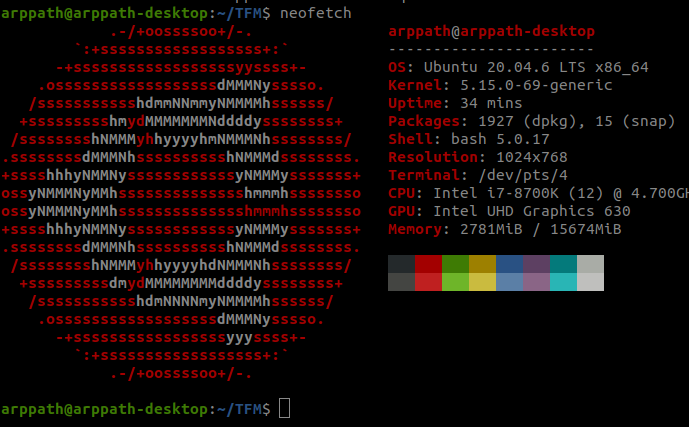
\includegraphics[width=12cm]{archivos/img/anexos/maquinaA.png}
    \caption{Especificaciones de la máquina A}
    \label{fig:maquinaA}
\end{figure}


\subsection{Especificaciones Máquina B}
\label{maquina_B}
\begin{itemize}
    \item Procesador: Intel i5-7500 (4) @ 3.800GHz
    \item Memoria: 31984MiB
    \item Gráfica: Intel HD Graphics 630
    \item Sistema operativo: Ubuntu 22.04.2 LTS x86\_64
\end{itemize}
\begin{figure}[ht!]
    \centering
    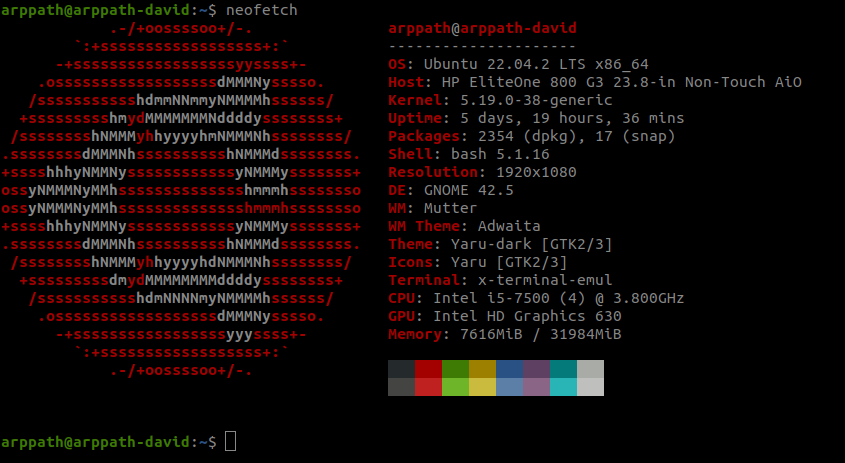
\includegraphics[width=12cm]{archivos/img/anexos/maquinaB.png}
    \caption{Especificaciones de la máquina B}
    \label{fig:maquinaB}
\end{figure}


\subsection{Especificaciones Máquina C}
\label{maquina_C}
\begin{itemize}
    \item Procesador: Intel(R) Core(TM) 12th Gen i7-1260P (16) CPU @ 4.70Ghz
    \item Memoria: 15674MiB
    \item Gráfica: Intel Alder Lake-P
    \item Sistema operativo: Ubuntu 22.04.2 LTS x86\_64
\end{itemize}
\begin{figure}[ht!]
    \centering
    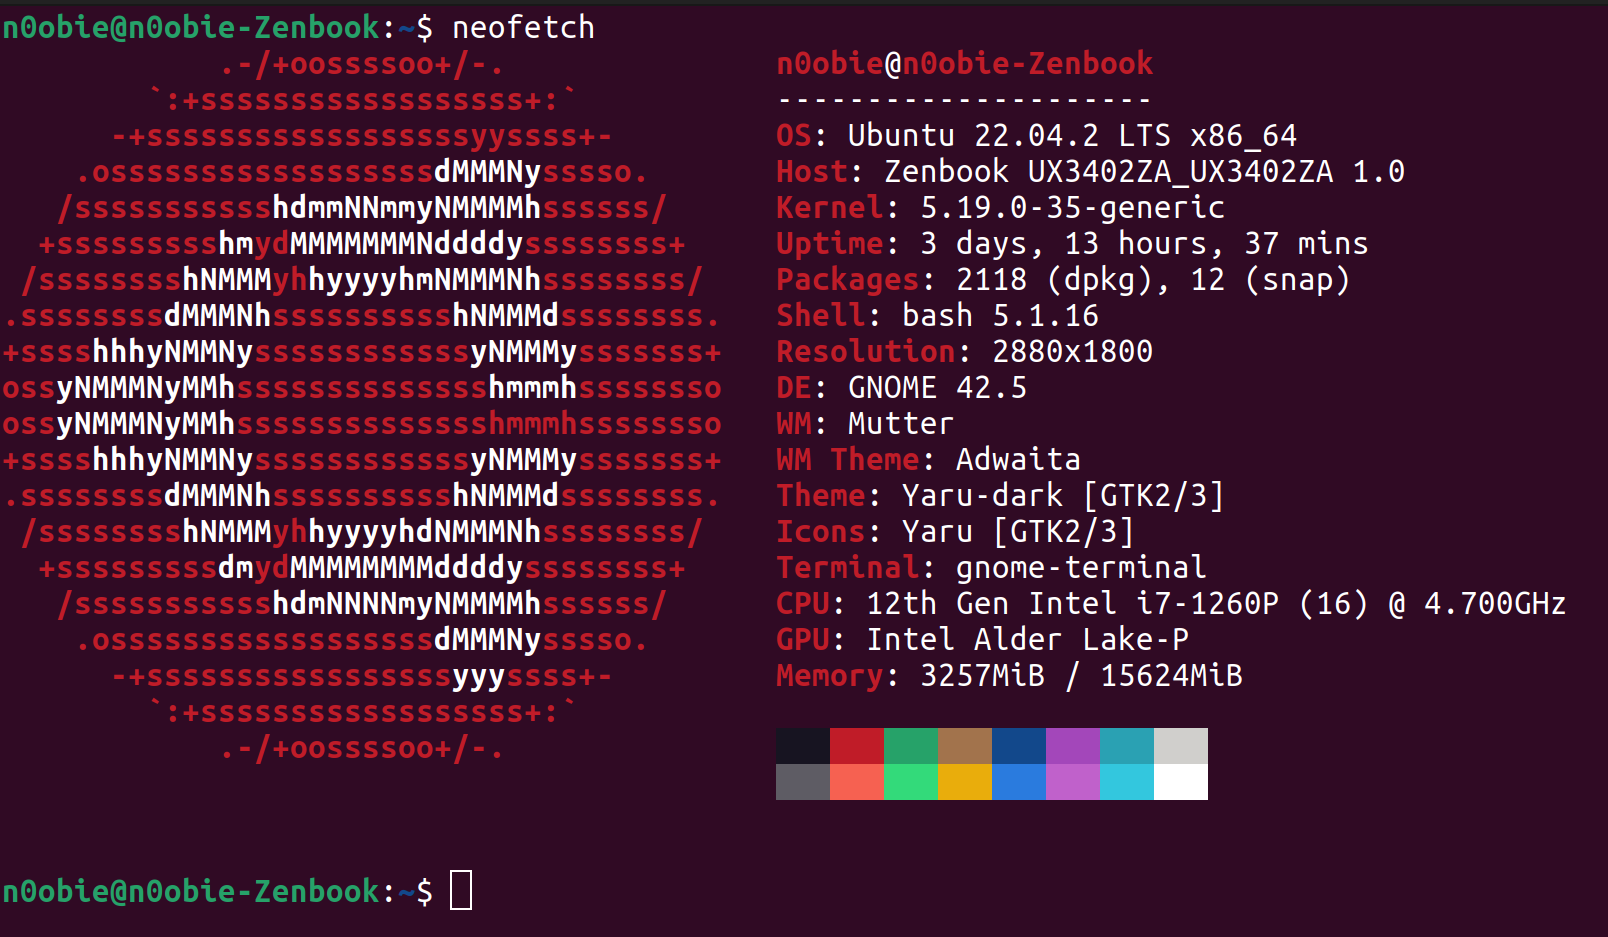
\includegraphics[width=12cm]{archivos/img/anexos/maquinaC.png}
    \caption{Especificaciones de la máquina C}
    \label{fig:maquinaC}
\end{figure}

%\chapter{Anexo II - Presupuesto}

En este anexo se quiere hacer una aproximación del presupuesto que tendría el proyecto llevado a cabo. Para ello, debemos hacer recuentro de cuantas horas efectivas se han dedicado al proyecto, dado que, si bien es cierto que el TFM se ha extendido el doble del tiempo que se había estimado, no se ha dedicado el doble de semanas para la realización del mismo, dado que se ha ido compaginando con otros proyectos en paralelo. También hay que tener en cuenta los medios que se han utilizado para el desarrollo, clasificándolos en elementos \textit{hardware} y en elementos \textit{softaware}.

\section{Duración del proyecto}

%Con el propósito de obtener el número de horas de trabajo por semana del proyecto en \textbf{promedio}, se va a realizar un diagrama de Gantt. De este modo se podrá apreciar la distribución de tareas a lo largo del \gls{tfm} y así ser capaces de obtener un número de horas de trabajo aproximado por semana.

Según se ha comentado anteriormente, con el propósito de obtener el número de horas \textbf{efectivas} dedicadas al proyecto, se va a realizar un diagrama de Gantt. De esta forma se pretende aclarar cuantas semanas se han dedicado a cada etapa del proyecto, y de este modo, poder llegar a estimar un número de horas efectivas de trabajo.\\
\\
Se quiere aclarar, que la duración del proyecto se ha extendido en el tiempo casi un año más de lo previsto, sin embargo, esta extensión temporal no ha sido completamente efectiva sobre el proyecto, dado que se ha ido compaginando con otros proyectos en paralelo. Se quiere de esta forma obtener, aproximadamente, una estimación temporal en semanas de cuanto ha llevado cada etapa del \gls{tfm}.\\
\\
Como se puede ver la etapa critica de este proyecto ha sido XXX

\newpage

\begin{figure}[ht!]
	\begin{center}
		\begin{tikzpicture}
			\begin{ganttchart}[
					hgrid,
					vgrid,
					y unit chart=.75cm,
					bar/.append style={fill=cyan!50},
					expand chart=\textwidth
				]{1}{15}
				\gantttitle{Semanas}{15} \\
				\gantttitlelist{1,...,15}{1} \\
				\ganttbar{Documentación y estudio}{1}{3} \\
				\ganttbar{Planificación}{1}{3} \ganttnewline
				\ganttbar{Diseño de los escenarios}{2}{3} \ganttnewline
				\ganttbar{Instalación del entornos de desarrollo}{4}{4} \ganttnewline
				\ganttbar{Aprendizaje de las herramientas}{4}{5} \ganttnewline
				\ganttbar{Desarrollo de los casos de uso}{5}{10} \ganttnewline
				\ganttbar{Valoración del desarrollo}{9}{12} \ganttnewline
				\ganttbar{Conclusiones y búsqueda de trabajo futuro}{12}{13} \\
				\ganttbar{Informe final}{13}{15}
			\end{ganttchart}
		\end{tikzpicture}
	\end{center}
	%\caption{Diagrama de Gantt del proyecto}
	\label{gantt}
\end{figure}

\begin{table}[ht!]
	\centering
	\begin{tabular}{|c|c|c|}
		\hline
		\rowcolor[HTML]{EFEFEF}
		\textbf{Número de horas totales} & \textbf{Horas por semana} & \textbf{Horas diarias} \\ \hline
		425h                             & $\approx$ 28h             & $\approx$ 4.2h         \\ \hline
	\end{tabular}
	\caption{Promedio de horas de trabajo }
	\label{dig:horasTrabajadas}
\end{table}

\section{Costes del proyecto}

El cálculo de los costes del proyecto se va a realizar diferenciando previamente por \textit{Hardware}, \textit{Software} y mano de obra. De esta manera, se pretende que los costes se desglosen aportando claridad sobre la cuantía total.

\vspace{0.5cm}

\begin{table}[ht]
	\centering
	\begin{tabular}{|c|r|}
		\hline
		\rowcolor[HTML]{EFEFEF}
		\textbf{Producto (IVA incluido)}               & \multicolumn{1}{c|}{\cellcolor[HTML]{EFEFEF}\textbf{Valor (€)}} \\ \hline
		Ordenador portátil Lenovo Legion               & 1349,00                                                         \\ \hline
		Ordenador de sobremesa                         & 1450,00                                                         \\ \hline
		Pantalla Lenovo L27i                           & 129,99                                                          \\ \hline
		Pantalla Benq 21"                              & 79,89                                                           \\ \hline
		Periféricos                                    & 150,00                                                          \\ \hline
		Infraestructura de Red (PLCs y Router Livebox) & 70,00                                                           \\ \hline
	\end{tabular}
	\caption{Presupuesto desglosado del Hardware}
	\label{tab:costesHardware}
\end{table}

\vspace{0.5cm}

Las licencias de software generalmente se venden por años, o por meses. Por ello, se ha calculado el precio equivalente asociado a la duración del \gls{tfg}.

\vspace{0.5cm}

\begin{table}[ht]
	\centering
	\begin{tabular}{|c|r|}
		\hline
		\rowcolor[HTML]{EFEFEF}
		\textbf{Producto (IVA incluido)}     & \multicolumn{1}{c|}{\cellcolor[HTML]{EFEFEF}\textbf{Valor (€)}} \\ \hline
		Microsoft Office                     & 300,00                                                          \\ \hline
		Adobe Photoshop y Adobe Premiere Pro & 241,96‬                                                          \\ \hline
	\end{tabular}
	\caption{Presupuesto desglosado del Software}
	\label{tab:costesSoftware}
\end{table}

\vspace{0.5cm}

Se han tomado de referencia los honorarios de un ingeniero junior, los cuales corresponden a 20€ la hora. Los costes del \textit{hardware} y \textit{software} se han agregado como un único elemento, añadiéndolo al presupuesto con el valor total del desglose de los productos indicados.

\vspace{0.5cm}

\begin{table}[ht]
	\centering
	\begin{tabular}{|c|r|r|r|}
		\hline
		\rowcolor[HTML]{EFEFEF}
		\textbf{Descripción (IVA incluido)} & \multicolumn{1}{c|}{\cellcolor[HTML]{EFEFEF}\textbf{Unidades}}     & \multicolumn{1}{c|}{\cellcolor[HTML]{EFEFEF}\textbf{Coste unitario (€)}} & \multicolumn{1}{c|}{\cellcolor[HTML]{EFEFEF}\textbf{Coste total (€)}} \\ \hline
		Material Hardware                   & 1                                                                  & 3228,89                                                                  & 3228,89                                                               \\ \hline
		Material Software                   & 1                                                                  & 541,96                                                                   & 541,96                                                                \\ \hline
		Mano de obra                        & 425                                                                & 20,00                                                                    & 8500,00                                                               \\ \hline
		Costes fijos (Luz, Internet)        & 4                                                                  & 76,00                                                                    & 304,00                                                                \\ \hline
		\rowcolor[HTML]{FFFFC7}
		\textbf{TOTAL}                      & \multicolumn{3}{r|}{\cellcolor[HTML]{FFFFC7}\textbf{12.574,85‬‬5 €‬}}                                                                                                                                                    \\ \hline
	\end{tabular}
	\caption{Presupuesto total con IVA}
	\label{tab:budget}
\end{table}
%\chapter{Anexo III - Manuales de usuario e Instalación}

En este anexo se incluirán todos los manuales de usuario e instalación sobre aquellas herramientas que se crean necesarias para el desarrollo y comprobación de funcionamiento del \gls{tfg}. De forma adicional, se comentará cómo funcionan los scripts de instalación generados para que cualquier persona interesada en replicar los distintos casos de uso, tenga un fácil acceso a ellos.

\section{Instalación de dependencias de los casos de uso}
\label{deps}

La motivación de esta sección es plasmar en un punto como hacer uso de las herramientas que se han dejado desarrolladas para la instalación de las dependencias de los casos de uso. Como ya se indicó en el Pliego de condiciones, al tener dos entornos de trabajo muy diferenciados se iban a crear dos máquinas virtuales (\ref{maquina_p4}, \ref{maquina_xdp})  para conseguir aislar todo posible conflicto de dependencias. A continuación, se indicará como instalar las dependencias asociadas a cada entorno.

\subsection{Instalación de dependencias máquina \glsentryshort{xdp}}

La tecnología XDP, al ser desarrollada propiamente en el Kernel de Linux, no necesitará de muchas dependencias para trabajar con ella. Todas las dependencias inducidas vienen por la necesidad de ciertos compiladores para establecer todo el proceso de compilación de un programa \gls{xdp}, desde su C restringido hasta su forma de bytecode. Para instalar dichas dependencias se necesitará haber descargado el repositorio de este \gls{tfg} en local. Esto se puede realizar según se indica en el bloque \ref{code:xdp_deps}.

\begin{lstlisting}[language= bash, style=Consola, caption={Descarga del repositorio del TFG},label=code:xdp_deps]
    # En caso de no tener "git" instalado lo podemos hacer de la siguiente forma
    sudo apt install -y git
    
    
    # Una vez que está instalado git, haremos un "clone" del repositorio
    git clone https://github.com/davidcawork/TFG.git
\end{lstlisting}

\vspace{0.5cm}

Una vez descargado el repositorio se debería encontrar un directorio llamado \gls{tfg} en el directorio donde se haya ejecutado dicho comando. El siguiente paso para instalar las dependencias, será movernos hasta el directorio de los casos de uso \gls{xdp} y lanzar el script de instalación con permisos de super-usuario según se indica en el bloque \ref{code:xdp_deps2}.

\begin{lstlisting}[language= bash, style=Consola, caption={Instalación de dependencias XDP},label=code:xdp_deps2]
    # Nos movemos al directorio de los casos de uso XDP
    cd TFG/src/use_cases/xdp/
    
    # Lanzamos el script de instalación con permisos de super usuario
    sudo ./install.sh
\end{lstlisting}

\vspace{0.5cm}
Este script de instalación añadirá los siguientes paquetes e inicializará el submódulo de la librería \texttt{libbpf}:

\begin{itemize}
    \item Paquetes necesarios para el proceso de compilación de programas \gls{xdp}: \texttt{clang llvm libelf-dev gcc-multilib}
    \item Paquete necesario para tener todos los archivos de cabecera del Kernel que se tenga instalado:
          \texttt{linux-tools-\$(uname -r)}
    \item Paquete necesario en caso de querer hacer debug vía excepciones con la herramienta perf: \texttt{linux-tools-generic}
\end{itemize}

Por último, se quiere comentar el hecho de que es muy recomendable tener una versión superior a la \texttt{v4.12.0} de iproute2 ya que en versiones anteriores no se da soporte para \gls{xdp}. En Ubuntu 18.04 ya viene por defecto una versión compatible con \gls{xdp} por lo que no será necesario actualizarla, más información en el punto \ref{iproute2}.


\subsection{Instalación de dependencias máquina P4}

El entorno de trabajo P4 es bastante áspero y complicado, ya que se requieren de numerosas dependencias para poder empezar a trabajar con la tecnología P4. Por ello, para la instalación del entorno de P4 se ha dejado un script de instalación en el directorio de los casos de uso P4, bajo la carpeta \texttt{vm} con el nombre de \texttt{install.sh}. En el repositorio oficial, hay un método de instalación similar pero enfocado a un aprovisionamiento de Vagrant\footnote{\url{https://www.vagrantup.com/}}. \\
\par
El equipo de \textit{p4lang} monta una máquina virtual personalizada que al parecer del autor de este \gls{tfg} es demasiado \textit{User Friendly} ya que deja poco margen de maniobra para hacer una instalación más perfilada a un entorno de desarrollo real. Por ello, se ha tenido que desarrollar un script propio para su instalación. Esta nueva vía de instalación fue ofrecida en forma de pull-request al equipo \textit{p4lang} se puede consultar \href{https://github.com/p4lang/tutorials/pull/261}{\textbf{aquí}}.\\
\par

En primer lugar, se debe descargar el repositorio de este \gls{tfg}. Si no lo ha hecho aún puede consultarlo en el bloque \ref{code:xdp_deps}. Acto seguido, se deberá navegar hasta el directorio de los casos de uso P4 y lanzar el script como se indica en el bloque \ref{code:p4_deps}.

\begin{lstlisting}[language= bash, style=Consola, caption={Instalación de dependencias P4},label=code:p4_deps]
    # Nos movemos al directorio de los casos de uso XDP
    cd TFG/src/use_cases/p4/
    
    # Lanzamos el script de instalación con permisos de super usuario
    sudo ./vm/install.sh -q
\end{lstlisting}

Este script de instalación añadirá los siguientes paquetes y herramientas necesarias para el desarrollo en P4:

\begin{itemize}
    \item Paquetes necesarios que son dependencias de las herramientas principales de P4env.
    \item Herramientas del P4env: \texttt{P4C PI P4Runtime}
    \item Paquetes necesarios para la prueba de P4: \texttt{Mininet BMV2 gRPC Protobuf}
\end{itemize}


%%%%%%%%%%%%%%%%%%%%%%%%%%%%%%%%%%%%%%%%%%%%%%%%%%%%%%%%%%%%%%%%%%%%%%%%%%%%%%%%%%%%%%%%%
\section{Herramienta \texttt{iproute2}}
\label{iproute2}
Se ha querido añadir esta sección, ya que la herramienta iproute2 va a ser fundamental a la hora de cargar los programas \gls{xdp} en el Kernel, consultar interfaces, o verificar en que \textit{Network namespace} se encuentra el usuario. Por todo lo anterior, la herramienta iproute2 será una de las piezas claves para gestión de las \textit{Network Namespaces}, y la verificación de los casos de uso.



\subsection{¿Qué es \texttt{iproute2?}}

Iproute2 es un paquete utilitario de herramientas para la gestión del \textit{Networking} en los sistemas Linux. Además, se encuentra ya en la mayoría de las distribuciones actuales. Sus desarrolladores principales son Alexey Kuznetsov y Stephen Hemminger, aunque hoy en día es un proyecto opensource donde cientos de personas contribuyen activamente en el repositorio\footnote{\url{https://github.com/shemminger/iproute2}}.  \\
\par
Actualmente, la versión más reciente de la herramienta es \texttt{v5.2.0}. Dicha versión será la que se utilizará en Ubuntu 18.04. El conjunto de utilidades que ofrece iproute2 está pensado para la sustitución de herramientas que se recogen en el paquete de \textbf{net-tools}, como por ejemplo a \texttt{ifconfig}, \texttt{route}, \texttt{netstat}, \texttt{arp}, etc. En la tabla \ref{tab:ipNettools} se pueden apreciar las herramientas de net-tools equivalentes en iproute2.

\begin{table}[ht]
    \centering
    \begin{tabular}{|c|c|}
        \hline
        \rowcolor[HTML]{C0C0C0}
        {\color[HTML]{000000} \textbf{net-tools}} & {\color[HTML]{000000} \textbf{iproute2}} \\ \hline
        \texttt{arp}                              & \texttt{ip neigh}                        \\ \hline
        \texttt{ifconfig}                         & \texttt{ip link}                         \\ \hline
        \texttt{ifconfig -a}                      & \texttt{ip addr}                         \\ \hline
        \texttt{iptunnel}                         & \texttt{ip tunnel}                       \\ \hline
        \texttt{route}                            & \texttt{ip route}                        \\ \hline
    \end{tabular}
    \caption{Comparativa de herramientas Iproute2 con paquete net-tools}
    \label{tab:ipNettools}
\end{table}

\subsection{¿Por qué necesitamos \texttt{iproute2}?}

Cuando se está trabajando con los programas XDP y se quiere comprobar su funcionamiento, se debe compilarlos. Esto se hará con los compiladores LLVM\footnote{\url{https://llvm.org/}} más clang\footnote{\url{https://clang.llvm.org/}}, como ya se comentaba en el estado del arte. Este proceso de compilación convertirá el código de los programas \gls{xdp}, en un \textit{bytecode} \gls{bpf}, y más tarde, se almacenará este \textit{bytecode} en un fichero de tipo \gls{elf}. Una vez compilados, se tendrá que anclarlos en el Kernel, y es  en este punto es donde entrará iproute2, ya que tiene un cargador \gls{elf} ( generalmente se trabajará con extensiones del tipo *.o ). \newline
\newline
Además, la herramienta iproute2 permite al usuario comprobar si una interfaz tiene cargado un programa \gls{xdp}. Arrojando en dicho caso, el identificador del programa \gls{xdp}, que tiene anclado la interfaz y si este programa está cargado de una forma nativa o de una forma genérica. Al final de la esta sección, se indicará cómo hacer esta comprobación.

\subsection{Estudio de compatibilidad de la herramienta \texttt{iproute2} en Ubuntu}

Al trabajar con esta herramienta para cargar programas XDP, se necesita  la versión que soporte el cargador ficheros \gls{elf}. Si usted tiene la versión de iproute2 que viene instalada por defecto en Ubuntu 16.04, le indicamos que aún no da soporte a \gls{xdp}. Inicialmente se buscó información relativa a partir de que versión se daba soporte a \gls{xdp} tanto en Ubuntu 16.04, como en Ubuntu 18.04. Como no se encontró información precisa sobre ello, se ha realizado un estudio de la compatibilidad de iproute2 a través de Ubuntu 16.04 y Ubuntu 18.04.\\
\par

Este estudio de compatibilidad se llevó a cabo descargando cada versión de iproute2, compilándola, e instalándola en nuestra máquina. Por último, para verificar si dicha versión daba soporte a \gls{xdp}, se comprobaba si un programa \gls{xdp} genérico que se sabía que funcionaba, cargaba o no, y si éste mostraba estadísticas sobre su carga. Más adelante, se indicará cómo compilar e instalar una versión en particular de iproute2.  \\
\par

Como se puede apreciar en la siguiente tabla \ref{tab:iproute}, en Ubuntu 16.04 a partir de la versión \texttt{v4.14.0} no existe compatibilidad. Esto es debido a que requiere librerías de enlazado extensible de formato (No \gls{elf} Support). Para resolver este requerimiento se debería añadir una versión más reciente de la librería \textbf{libelf\_dev}. Se puede agregar dicha librería, pero al hacerlo aparecerán dependencias que se van ramificando una a una llegando a librerías más sensibles para nuestro sistema como \textbf{libc6}, por lo que se decidió no comprobar el funcionamiento añadiendo las nuevas librerías requeridas para no comprometer el sistema.


\begin{table}[ht]
    \centering
    \resizebox{\textwidth}{!}{%
        \begin{tabular}{|l|c|c|c|c|c|c|c|c|c|c|c|c|c|}
            \hline
            {\color[HTML]{333333} \textbf{Versiones IProute2}} & \multicolumn{1}{l|}{\cellcolor[HTML]{6A8AE5}v4.9.0}        & \multicolumn{1}{l|}{\cellcolor[HTML]{6A8AE5}v4.10.0}       & \multicolumn{1}{l|}{\cellcolor[HTML]{6A8AE5}v4.11.0}       & \multicolumn{1}{l|}{\cellcolor[HTML]{6A8AE5}v4.12.0} & \multicolumn{1}{l|}{\cellcolor[HTML]{6A8AE5}v4.13.0} & \multicolumn{1}{l|}{\cellcolor[HTML]{6A8AE5}v4.14.0} & \multicolumn{1}{l|}{\cellcolor[HTML]{6A8AE5}v4.15.0} & \multicolumn{1}{l|}{\cellcolor[HTML]{6A8AE5}v4.16.0} & \multicolumn{1}{l|}{\cellcolor[HTML]{6A8AE5}v4.17.0} & \multicolumn{1}{l|}{\cellcolor[HTML]{6A8AE5}v4.18.0} & \multicolumn{1}{l|}{\cellcolor[HTML]{6A8AE5}v4.20.0} & \multicolumn{1}{l|}{\cellcolor[HTML]{6A8AE5}v5.1.0} & \multicolumn{1}{l|}{\cellcolor[HTML]{6A8AE5}v5.2.0} \\ \hline
            \rowcolor[HTML]{FD6864}
            \cellcolor[HTML]{FFC702}Ubuntu 16.04               & \cellcolor[HTML]{67FD9A}{\color[HTML]{6665CD} No XDP supp} & \cellcolor[HTML]{67FD9A}{\color[HTML]{6665CD} No XDP supp} & \cellcolor[HTML]{67FD9A}{\color[HTML]{6665CD} No XDP supp} & \cellcolor[HTML]{67FD9A}{\color[HTML]{036400} Si}    & \cellcolor[HTML]{67FD9A}{\color[HTML]{036400} Si}    & {\color[HTML]{9A0000} No}                            & {\color[HTML]{9A0000} No}                            & {\color[HTML]{9A0000} No}                            & {\color[HTML]{9A0000} No}                            & {\color[HTML]{9A0000} No}                            & {\color[HTML]{9A0000} No}                            & {\color[HTML]{9A0000} No}                           & {\color[HTML]{9A0000} No}                           \\ \hline
            \cellcolor[HTML]{9870D0}Ubuntu 18.04               & -                                                          & -                                                          & -                                                          & -                                                    & -                                                    & -                                                    & \cellcolor[HTML]{67FD9A}{\color[HTML]{036400} Si}    & \cellcolor[HTML]{67FD9A}{\color[HTML]{036400} Si}    & \cellcolor[HTML]{67FD9A}{\color[HTML]{036400} Si}    & \cellcolor[HTML]{67FD9A}{\color[HTML]{036400} Si}    & \cellcolor[HTML]{67FD9A}{\color[HTML]{036400} Si}    & \cellcolor[HTML]{67FD9A}{\color[HTML]{036400} Si}   & \cellcolor[HTML]{67FD9A}{\color[HTML]{036400} Si}   \\ \hline
        \end{tabular}%
    }
    \caption{Estudio de compatibilidad de la herramienta Iproute2}
    \label{tab:iproute}
\end{table}

\begin{figure}
    \centering
    \begin{tikzpicture}[node distance=2cm, auto]
        % Cuadros
        \node (deps) [rectvioleta,text width=3cm] {\texttt{libelf\_dev} \par};
        \node (deps2) [rectvioleta,below of=deps,text width=3cm] { \texttt{libelf1} \par};
        \node (deps3) [rectvioleta,right of=deps2,xshift=3cm, text width=3cm] { \texttt{zliblg} \par};
        \node (harddep) [rectnaranja,below of=deps2,text width=3cm]{ \texttt{libc6} \par};
        % Flechas
        \draw[arrow] (deps) -- (deps2);
        \draw[arrow] (deps2) -- (deps3);
        \draw[arrow] (deps2) -- (harddep);

    \end{tikzpicture}
    \caption{Ramificación de dependencias de Iproute2.}
    \label{fig:DependenciasIproute}
\end{figure}

\newpage

\subsection{Compilación e instalación de \texttt{iproute2}}
El proceso es prácticamente análogo tanto en Ubuntu 16.04 como en Ubuntu 18.04, salvo por una única diferencia que se indicará más adelante. Ahora se mostrarán los pasos necesarios para la compilación e instalación de una versión, en concreto de la herramienta iproute2.

\begin{itemize}
    \item En primer lugar, se necesitará de instalar los paquetes necesarios para la configuración previa a la compilación.
          \begin{itemize}
              \item \texttt{bison}, es un herramienta generadora de analizadores sintácticos de propósito general.
              \item \texttt{flex}, es una herramienta para generar programas que reconocen patrones léxicos en el texto.
              \item \texttt{libmnl-dev}, es una librería de espacio de usuario orientada a los desarrolladores de Netlink. Netlink\footnote{\url{https://www.man7.org/linux/man-pages/man7/netlink.7.html}} es una interfaz entre espacio de usuario y espacio de Kernel vía sockets.

              \item \texttt{libdb5.3-dev}, éste es un paquete de desarrollo que contiene los archivos de cabecera y librerías estáticas necesarias para la BBDD de Berkley (\textit{Key/Value}).

              \item Se entiende que se tiene el paquete \texttt{wget}. En caso de no tenerlo, solo se deberá añadir para poder descargar la herramienta.
          \end{itemize}
\end{itemize}
\begin{lstlisting}[language= bash, style=Consola2, caption={Instalación de las dependencias de Iproute2},label=code:iproute2_deps]
   sudo apt-get install bison flex libmnl-dev libdb5.3-dev
\end{lstlisting}
\begin{itemize}
    \item En segundo lugar, se debe descargar el comprimido de la herramienta iproute2. Al haber varios paquetes, se descargará aquel cuya versión sea con la que se quiere trabajar. Podemos descargarlas desde aquí: \href{https://mirrors.edge.kernel.org/pub/linux/utils/net/iproute2/}{\textbf{kernel.org}}.
\end{itemize}
\begin{lstlisting}[language= bash, style=Consola, caption={Obtención del source de Iproute2},label=code:iproute2_src]
   wget -c http://ftp.iij.ad.jp/pub/linux/kernel/linux/utils/net/iproute2/iproute2-4.15.0.tar.gz
\end{lstlisting}

\begin{itemize}
    \item En tercer lugar, se debe descomprimir el comprimido de la herramienta. Acto seguido, se procederá a configurarla, compilarla e instalarla.
\end{itemize}

\begin{lstlisting}[language= bash, style=Consola, caption={Compilación e instalación de Iproute2},label=code:iproute2_install]
   # Se descomprime y se entra al directorio
   tar -xvfz $(tar).tar.gz && cd $tar
   
   # Se configura
   ./configura
   
   # Se compila e instala, para añadir el nuevo binario en el path
   sudo make
   sudo make install
\end{lstlisting}
\subsubsection{Diferencias con Ubuntu 18.04}

La única diferencia en el proceso de instalación de la herramienta de iproute2 en Ubuntu 18.04, es añadir un paquete extra antes de proceder a configurar, compilar e instalar. El paquete extra es \textbf{pkg-config}; de no añadirlo fallará al lanzar el script de configuración y hacer el build.
\begin{lstlisting}[language= bash, style=Consola, caption={Instalación de las dependencias de Iproute2 - Ubuntu 18.04},label=code:iproute2_deps18]
    sudo apt-get install bison flex libmnl-dev libdb5.3-dev pkg-config
\end{lstlisting}

\subsection{Comandos útiles con \texttt{iproute2}}

A continuación, se indican los comandos más frecuentes con la herramienta iproute2. Todos ellos han sido utilizados en el proceso de desarrollo del proyecto y en el proceso de verificación de los distintos casos de uso. Por ello, se considera que este apartado puede ser de gran utilidad para el lector que nunca ha trabajado con esta herramienta.

\begin{lstlisting}[language= bash, style=Consola, caption={Comandos útiles con iproute2},label=code:iproute2_use]
    # Listar interfaces y ver direcciones asignadas
    ip addr show
    
    # Poner/Quitar dirección a una interfaz
    ip addr add {IP} dev {interfaz}
    ip addr del {IP} dev {interfaz}
    
    # Levantar/deshabilitar una interfaz 
    ip link set {interfaz} up/down
    
    # Listar rutas
    ip route list 
    
    # Obtener ruta para una determinada dirección IP
    ip route get {IP}
    
    # Listar Network namespace con nombre
    ip netns list
    

\end{lstlisting}
\newpage
%%%%%%%%%%%%%%%%%%%%%%%%%%%%%%%%%%%%%%%%%%%%%%%%%%%%%%%%%%%%%%%%%%%%%%%%%%%%%%%%%%%%%%%%%%%%%%%%%%

\section{Herramienta \texttt{tcpdump}}
\label{tcpdump}
La motivación de añadir esta sección ha sido la de tener un punto de encuentro para las personas que nunca han utilizado tcpdump, ya que a lo largo de todas las secciones del proyecto, se hará uso de esta herramienta para verificar si los casos de uso realmente funcionan según lo esperado.

\subsection{¿Qué es \texttt{tcpdump}?}

Tcpdump es un analizador de tráfico para inspeccionar los paquetes entrantes y salientes de una interfaz. La peculiaridad de esta herramienta es que funciona por línea de comandos, y tiene soporte en la mayoría de sistemas UNIX\footnote{Unix es un sistema operativo desarrollado en 1969 por un grupo de empleados de los laboratorios Bell}, como por ejemplo Linux, macOS y OpenWrt. La herramienta está escrita en lenguaje C por lo que tiene un gran rendimiento y hace uso de libpcap\footnote{\url{https://github.com/the-tcpdump-group/libpcap}} como vía para interceptar los paquetes.\\
\par
La herramienta fue escrita en el año 1988 por trabajadores de los laboratorios de Berkeley. Actualmente, cuenta con una gran comunidad de desarrolladores a su espalda en su repositorio oficial\footnote{\url{https://github.com/the-tcpdump-group/tcpdump}} sacando nuevas actualizaciones de forma periódica (última versión \texttt{
    v4.9.3}).

\subsection{¿Por qué necesitamos \texttt{tcpdump}?}

Hoy en día, es un hecho que en la mayoría de los casos no se suele desarrollar en una misma máquina. Se suele utilizar contenedores o máquina virtuales con el propósito de tener acotado el escenario de desarrollo. Por ello, se suele trabajar la mayoría de veces de forma remota, conectándose a la máquina/contenedor haciendo uso de ssh\footnote{\url{https://www.ssh.com/ssh/}}.\\
\par

Esto implica numerosas ventajas, pero también complicaciones. Si una persona no sabe configurar un \textit{X Server} con el cual ejecutar aplicaciones gráficas de forma remota, no podría correr por ejemplo Wireshark. En este punto entra tcpdump, el cual no requiere de ningún tipo de configuración extra para poder ser ejecutado de forma remota. Esto añadido al hecho de su rápida puesta en marcha, con respecto a otros \textit{sniffers} como Wireshark, han convertido a tcpdump en una herramienta fundamental en los procesos de verificación de los casos de uso.

\subsection{Instalación de \texttt{tcpdump}}

Como ya se comentaba en la introducción, esta herramienta tiene un gran soporte entre los sistemas UNIX, por lo que generalmente suele encontrarse ya instalado en la mayoría de distribuciones Linux. De no tenerla instalada, siempre se podrá instalar de la siguiente forma \ref{code:tcpdump}.

\begin{lstlisting}[language= bash, style=Consola2, caption={Instalación de Tcpdump},label=code:tcpdump]
    sudo apt install tcpdump
\end{lstlisting}

\subsection{Comandos útiles con \texttt{tcpdump}}

A continuación, se indican los comandos más frecuentes con la herramienta tcpdump. Todos ellos han sido utilizados en su mayoría en el proceso de verificación de los distintos casos de uso. Por lo tanto, se considera que este apartado puede ser de gran utilidad para el lector que nunca ha trabajado con esta herramienta. Además, se recomienda al lector consultar su \textit{man-page}\footnote{\url{https://linux.die.net/man/8/tcpdump}} donde podrá encontrar información más detallada sobre el uso básico de tcpdump.

\begin{lstlisting}[language= bash, style=Consola2, caption={Comandos útiles con Tcpdump},label=code:tcpdump_use]
    # Indicar sobre que Interfaz se quiere escuchar
    tcpdump -i {Interfaz}
    
    # Almacenar la captura a un archivo para su posterior análisis
    tcpdump -w fichero.pcap -i {Interfaz}
    
    # Leer captura desde un archivo
    tcpdump -r fichero.pcap
    
    # Filtrar por puerto
    tcpdump -i {Interfaz} port {Puerto}
    
    # Filtrar por dirección IP destino/origen
    tcpdump -i {Interfaz} dst/src {IP}
    
    #Filtrar por protocolo
    tcpdump -i {Interfaz} {protocolo}
    
    # Listar interfaces disponibles
    tcpdump -D
    
     # Limitar el número de paquetes a escuchar
    tcpdump -i {Interfaz} -c {Número de paquetes}
\end{lstlisting}
\vspace{1cm}
\begin{figure}[ht]
    \centering
    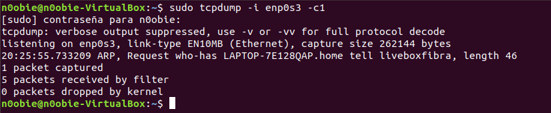
\includegraphics[width=14cm]{archivos/img/anexos/tcpdump_cli_edited.png}
    \caption{Interfaz CLI de Tcpdump}
    \label{tcpdumpCli}
\end{figure}

%%%%%%%%%%%%%%%%%%%%%%%%%%%%%%%%%%%%%%%%%%%%%%%%%%%%%%%%%%%%%%%%%%%%%%%%%%%%%%%%%%%%%%%%%%%%%%%%%%
\section{Herramienta Mininet}
\label{sec:ToolsMininet}
La motivación de añadir esta sección es la de poder indicar al lector como se ha instalado la herramienta de Mininet en las distintas máquinas descritas en el pliego de condiciones (Anexo \ref{ch:anexoPliegoCondiciones}). Todo el proceso de instalación se ha llevado acabo en una máquina Linux, con las especificaciones indicadas en la siguiente tabla (Tabla \ref{tab:ToolsMininet}).

\begin{table}[ht!]
    \centering
    \resizebox{0.6\columnwidth}{!}{%
        \begin{tabular}{|c|c|c|c|}
            \hline
            \rowcolor[HTML]{EFEFEF}
            \textbf{Distribución Linux} & \textbf{Cores} & \textbf{Memoria} & \textbf{Disco} \\ \hline
            Ubuntu 22.04 LTS            & 2              & 4096 MiB         & 40 GiB         \\ \hline
        \end{tabular}%
    }
    \caption{Especificaciones máquina de instalación Mininet}
    \label{tab:ToolsMininet}
\end{table}

Para la instalación necesitaremos de conectividad a Internet y de la herramienta \texttt{git} para clonar el repositorio de \texttt{Mininet}. En caso de no tener la herramienta de \texttt{git}, podremos instalarla ejecutando el comando del bloque de código \ref{code:git_install}.

\begin{lstlisting}[language= bash, style=Consola2, caption={Instalación de la herramienta git},label=code:git_install]
    # El parametro -y se indica para confirmar la instalación de la herramienta
    sudo apt install -y git 
\end{lstlisting}
\vspace{1cm}

Una vez disponemos de la herramienta \texttt{git} para clonar el repositorio de \texttt{Mininet}, vamos a clonarlo, y lanzar el script de instalación que incorpora junto al source para instalar la herramineta. A continuación, en el bloque de código \ref{code:Mininet_install} se indica los comandos ejecutados para instalar la herrmaienta de \texttt{Mininet}.


\begin{lstlisting}[language= bash, style=Consola2, caption={Instalación de la herramienta Mininet},label=code:Mininet_install]
    # Clonamos el repositorio de Mininet
    git clone https://github.com/davidcawork/mininet.git

    # Accedemos al directorio
    cd mininet

    # Lanzamos el script de instalación (Openflow 1.3 - Ryu - Wireshark dissector)
    sudo util/install.sh -3fmnyv
\end{lstlisting}
\vspace{1cm}


%%%%%%%%%%%%%%%%%%%%%%%%%%%%%%%%%%%%%%%%%%%%%%%%%%%%%%%%%%%%%%%%%%%%%%%%%%%%%%%%%%%%%%%%%%%%%%%%%%


% Contra portada

\includepdf[pages={4}]{include/portada/portada_uah_eps_MUIT_TFM.pdf}


\end{document}
